\documentclass[twoside,11pt]{article}
\pagestyle{myheadings}
\usepackage{epsfig}

%------------------------------------------------------------------------------
% Add any \newcommand or \newenvironment commands here
\newcommand{\about}{$\sim$}
\newcommand{\eg}{{\it e.g.}}
\newcommand{\ie}{{\it i.e.}}
\newcommand{\mic}{\mbox{\,${\mu}$m}}               % microns
\newcommand{\arcmin}{{$^\prime$}}
\newcommand{\degr}{\mbox{\,$^\circ$}}               % degrees sign
%------------------------------------------------------------------------------

% -----------------------------------------------------------------------------
% ? Document identification
\newcommand{\stardoccategory}  {Starlink Cookbook}
\newcommand{\stardocinitials}  {SC}
\newcommand{\stardocsource}    {sc\stardocnumber}
\newcommand{\stardocnumber}    {11.1}
\newcommand{\stardocauthors}   {G. Sandell \\ \jac}
\newcommand{\stardocdate}      {1 August 1997}
\newcommand{\stardoctitle}     {The SCUBA mapping cookbook\\[2ex]
                                A first step to proper map reduction}
\newcommand{\stardocversion}   {\ }
\newcommand{\stardocmanual}    {\ }
\newcommand{\stardocabstract}  {[Text of abstract]}
% ? End of document identification
 
% A new environment for quoting verbatim
% Environment for indenting and using a small font.
\newenvironment{myquote}{\begin{quote}\begin{small}}{\end{small}\end{quote}}
 
\newcommand{\text}[1]{{\small \texttt{#1}}}
 
% SCUBA reference
\newcommand{\scuba}{\htmladdnormallink{SCUBA}{http://www.jach.hawaii.edu/JCMT/}}

 
% Starlink Package names
\newcommand{\starlink}{\htmladdnormallink{Starlink}{http://star-www.rl.ac.uk/}}
 
% set up some common package names
\newcommand{\Kappa}{\xref{\textsc{Kappa}}{sun95}{}}
\newcommand{\Figaro}{\xref{\textsc{Figaro}}{sun86}{}}
\newcommand{\gaia}{\xref{\textsc{Gaia}}{sun214}{}}
\newcommand{\convert}{\xref{\textsc{Convert}}{sun55}{}}
\newcommand{\fluxes}{\xref{\textsc{Fluxes}}{sun213}{}}
\newcommand{\Iras}{\xref{\textsc{Iras90}}{sun163}{}}
\newcommand{\ndf}{\xref{NDF}{sun33}{}}
\newcommand{\agi}{\xref{AGI}{sun48}{}}
\newcommand{\surf}{\xref{\textsc{Surf}}{sun216}{}}
\newcommand{\Specdre}{\xref{\textsc{Specdre}}{sun140}{}}
\newcommand{\jcmtdr}{\xref{\textsc{JCMTdr}}{sun132}{}}
\newcommand{\nod}{\textsc{nod2}}
\newcommand{\ESP}{\xref{ESP}{sun180}{}}
\newcommand{\GKS}{\xref{GKS}{sun83}{}}

% Application tasks
\newcommand{\task}[1]{\textsf{#1}}
 
% ADAM parameters
\newcommand{\param}[1]{\texttt{#1}}
 
% SURF tasks
\newcommand{\rebin}{\xref{\task{rebin}}{sun216}{REBIN}}
\newcommand{\bolrebin}{\xref{\task{bolrebin}}{sun216}{BOLREBIN}}
\newcommand{\intrebin}{\xref{\task{intrebin}}{sun216}{INTREBIN}}
\newcommand{\chgqual}{\xref{\task{change\_\-qua\-lity}}{sun216}{CHANGE_QUALITY}}
\newcommand{\chgflat}{\xref{\task{change\_flat}}{sun216}{CHANGE_FLAT}}
\newcommand{\chgpnt}{\xref{\task{change\_pointing}}{sun216}{CHANGE_POINTING}}
\newcommand{\chgdata}{\xref{\task{change\_data}}{sun216}{CHANGE_DATA}}
\newcommand{\resw}{\xref{\task{reduce\_switch}}{sun216}{REDUCE_SWITCH}}
\newcommand{\flatf}{\xref{\task{flatfield}}{sun216}{FLATFIELD}}
\newcommand{\skydip}{\xref{\task{skydip}}{sun216}{SKYDIP}}
\newcommand{\scuphot}{\xref{\task{scuphot}}{sun216}{SCUPHOT}}
\newcommand{\ext}{\xref{\task{extinction}}{sun216}{EXTINCTION}}
\newcommand{\scuquick}{\xref{\task{scuquick}}{sun216}{SCUQUICK}}
\newcommand{\scuhelp}{\xref{\task{scuhelp}}{sun216}{SCUHELP}}
\newcommand{\remsky}{\xref{\task{remsky}}{sun216}{REMSKY}}
\newcommand{\scuover}{\xref{\task{scuover}}{sun216}{SCUOVER}}
\newcommand{\extdata}{\xref{\task{extract\_data}}{sun216}{EXTRACT_DATA}}
\newcommand{\sculog}{\xref{\task{sculog}}{sun216}{SCULOG}}
\newcommand{\scucat}{\xref{\task{scucat}}{sun216}{SCUCAT}}
\newcommand{\photsum}{\xref{\task{photsum}}{sun216}{PHOTSUM}}
\newcommand{\mapsum}{\xref{\task{mapsum}}{sun216}{MAPSUM}}
\newcommand{\pointsum}{\xref{\task{pointsum}}{sun216}{POINTSUM}}
\newcommand{\qdraw}{\xref{\task{qdraw}}{sun216}{QDRAW}}
\newcommand{\sigclip}{\xref{\task{sigclip}}{sun216}{SIGCLIP}}
\newcommand{\restore}{\xref{\task{restore}}{sun216}{RESTORE}}
\newcommand{\sdip}{\xref{\task{sdip}}{sun216}{SDIP}}
\newcommand{\scupa}{\xref{\task{scupa}}{sun216}{SCUPA}}
\newcommand{\obssum}{\xref{\task{obssum}}{sun216}{OBSSUM}}
 
% Non surf tasks

% KAPPA 
\newcommand{\display}{\xref{\task{display}}{sun95}{DISPLAY}}
\newcommand{\aperadd}{\xref{\task{aperadd}}{sun95}{APERADD}}
\newcommand{\linplot}{\xref{\task{linplot}}{sun95}{LINPLOT}}
\newcommand{\mlinplot}{\xref{\task{mlinplot}}{sun95}{MLINPLOT}}
\newcommand{\drawsig}{\xref{\task{drawsig}}{sun95}{DRAWSIG}}
\newcommand{\centroid}{\xref{\task{centroid}}{sun95}{CENTROID}}
\newcommand{\hislist}{\xref{\task{hislist}}{sun95}{HISLIST}}
\newcommand{\globals}{\xref{\task{globals}}{sun95}{GLOBALS}}
\newcommand{\setaxis}{\xref{\task{setaxis}}{sun95}{SETAXIS}}
\newcommand{\kstest}{\xref{\task{kstest}}{sun95}{KSTEST}}
\newcommand{\stats}{\xref{\task{stats}}{sun95}{STATS}}
\newcommand{\thresh}{\xref{\task{thresh}}{sun95}{THRESH}}
\newcommand{\setbb}{\xref{\task{setbb}}{sun95}{SETBB}}
\newcommand{\fitslist}{\xref{\task{fitslist}}{sun95}{FITSLIST}}
\newcommand{\fitsedit}{\xref{\task{fitsedit}}{sun95}{FITSEDIT}}
\newcommand{\setvar}{\xref{\task{setvar}}{sun95}{SETVAR}}
\newcommand{\ndfcopy}{\xref{\task{ndfcopy}}{sun95}{NDFCOPY}}
\newcommand{\gdset}{\xref{\task{gdset}}{sun95}{GDSET}}
\newcommand{\idset}{\xref{\task{idset}}{sun95}{IDSET}}
\newcommand{\ovset}{\xref{\task{ovset}}{sun95}{OVSET}}
\newcommand{\gdnames}{\xref{\task{gdnames}}{sun95}{GDNAMES}}
\newcommand{\gdclear}{\xref{\task{gdclear}}{sun95}{GDCLEAR}}
\newcommand{\cursor}{\xref{\task{cursor}}{sun95}{CURSOR}}
\newcommand{\flip}{\xref{\task{flip}}{sun95}{FLIP}}
\newcommand{\cadd}{\xref{\task{cadd}}{sun95}{CADD}}
\newcommand{\cdiv}{\xref{\task{cdiv}}{sun95}{CDIV}}
\newcommand{\Div}{\xref{\task{div}}{sun95}{DIV}}
\newcommand{\cmult}{\xref{\task{cmult}}{sun95}{CMULT}}
\newcommand{\mult}{\xref{\task{mult}}{sun95}{MULT}}
\newcommand{\add}{\xref{\task{add}}{sun95}{ADD}}
\newcommand{\sub}{\xref{\task{sub}}{sun95}{SUB}}
\newcommand{\csub}{\xref{\task{csub}}{sun95}{CSUB}}
\newcommand{\psf}{\xref{\task{psf}}{sun95}{PSF}}
\newcommand{\glitch}{\xref{\task{glitch}}{sun95}{GLITCH}}
\newcommand{\setunits}{\xref{\task{setunits}}{sun95}{SETUNITS}}
\newcommand{\fitstext}{\xref{\task{fitstext}}{sun95}{FITSTEXT}}
\newcommand{\fitsmod}{\xref{\task{fitsmod}}{sun95}{FITSMOD}}
\newcommand{\fitshead}{\xref{\task{fitshead}}{sun95}{FITSHEAD}}
\newcommand{\lutbgyrw}{\xref{\task{lutbgyrw}}{sun95}{LUTBGYRW}}
\newcommand{\contour}{\xref{\task{contour}}{sun95}{CONTOUR}}
\newcommand{\contover}{\xref{\task{contover}}{sun95}{CONTOVER}}
\newcommand{\turbocont}{\xref{\task{turbocont}}{sun95}{TURBOCONT}}
\newcommand{\mosaic}{\xref{\task{mosaic}}{sun95}{MOSAIC}}
\newcommand{\pixdupe}{\xref{\task{pixdupe}}{sun95}{PIXDUPE}}
\newcommand{\rotate}{\xref{\task{rotate}}{sun95}{ROTATE}}
\newcommand{\setbound}{\xref{\task{setbound}}{sun95}{SETBOUND}}
\newcommand{\slide}{\xref{\task{slide}}{sun95}{SLIDE}}
\newcommand{\gausmooth}{\xref{\task{gausmooth}}{sun95}{GAUSMOOTH}}
\newcommand{\median}{\xref{\task{median}}{sun95}{MEDIAN}}
\newcommand{\memd}{\xref{\task{mem2d}}{sun95}{MEM2D}}
\newcommand{\axlabel}{\xref{\task{axlabel}}{sun95}{AXLABEL}}
\newcommand{\axunits}{\xref{\task{axunits}}{sun95}{AXUNITS}}
\newcommand{\setlabel}{\xref{\task{setlabel}}{sun95}{SETLABEL}}
\newcommand{\settitle}{\xref{\task{settitle}}{sun95}{SETTITLE}}
\newcommand{\histogram}{\xref{\task{histogram}}{sun95}{HISTOGRAM}}
\newcommand{\normalize}{\xref{\task{normalize}}{sun95}{NORMALIZE}}

% Convert
\newcommand{\ndffits}{\xref{\task{ndf2fits}}{sun55}{NDF2FITS}}
\newcommand{\ndfascii}{\xref{\task{ndf2ascii}}{sun55}{NDF2ASCII}}

% FIGARO
\newcommand{\wdfits}{\xref{\task{wdfits}}{sun86}{WDFITS}}
\newcommand{\istat}{\xref{\task{istat}}{sun86}{ISTAT}}
\newcommand{\delobj}{\xref{\task{delobj}}{sun86}{DELOBJ}}
\newcommand{\copobj}{\xref{\task{copobj}}{sun86}{COPOBJ}}
\newcommand{\image}{\xref{\task{image}}{sun86}{IMAGE}}
\newcommand{\bclean}{\xref{\task{bclean}}{sun86}{BCLEAN}}
\newcommand{\ystract}{\xref{\task{ystract}}{sun86}{YSTRACT}}

% IRAS90
\newcommand{\skypos}{\xref{\task{skypos}}{sun163}{SKYPOS}}
\newcommand{\skygrid}{\xref{\task{skygrid}}{sun163}{SKYGRID}}
\newcommand{\skyphot}{\xref{\task{skyphot}}{sun163}{SKYPHOT}}


% Misc
\newcommand{\hdstrace}{\xref{\task{hdstrace}}{sun102}{}}
\newcommand{\psmerge}{\xref{\task{psmerge}}{sun164}{}}
\newcommand{\fitgauss}{\xref{\task{fitgauss}}{sun140}{FITGAUSS}}
\newcommand{\gaufit}{\xref{\task{gaufit}}{sun180}{GAUFIT}}

% JAC

\newcommand{\jac}{\htmladdnormallink{Joint Astronomy Centre}{http://www.jach.hawaii.edu},
 Hilo, Hawaii}


 
% -----------------------------------------------------------------------------
 
\newcommand{\stardocname}{\stardocinitials /\stardocnumber}
\markboth{\stardocname}{\stardocname}
\setlength{\textwidth}{160mm}
\setlength{\textheight}{230mm}
\setlength{\topmargin}{-2mm}
\setlength{\oddsidemargin}{0mm}
\setlength{\evensidemargin}{0mm}
\setlength{\parindent}{0mm}
\setlength{\parskip}{\medskipamount}
\setlength{\unitlength}{1mm}
 
% -----------------------------------------------------------------------------
%  Hypertext definitions.
%  ======================
%  These are used by the LaTeX2HTML translator in conjunction with star2html.
 
%  Comment.sty: version 2.0, 19 June 1992
%  Selectively in/exclude pieces of text.
%
%  Author
%    Victor Eijkhout                                      <eijkhout@cs.utk.edu>
%    Department of Computer Science
%    University Tennessee at Knoxville
%    104 Ayres Hall
%    Knoxville, TN 37996
%    USA
 
%  Do not remove the %\begin{rawtex} and %\end{rawtex} lines (used by 
%  star2html to signify raw TeX that latex2html cannot process).
%\begin{rawtex}
\makeatletter
\def\makeinnocent#1{\catcode`#1=12 }
\def\csarg#1#2{\expandafter#1\csname#2\endcsname}
 
\def\ThrowAwayComment#1{\begingroup
    \def\CurrentComment{#1}%
    \let\do\makeinnocent \dospecials
    \makeinnocent\^^L% and whatever other special cases
    \endlinechar`\^^M \catcode`\^^M=12 \xComment}
{\catcode`\^^M=12 \endlinechar=-1 %
 \gdef\xComment#1^^M{\def\test{#1}
      \csarg\ifx{PlainEnd\CurrentComment Test}\test
          \let\html@next\endgroup
      \else \csarg\ifx{LaLaEnd\CurrentComment Test}\test
            \edef\html@next{\endgroup\noexpand\end{\CurrentComment}}
      \else \let\html@next\xComment
      \fi \fi \html@next}
}
\makeatother
 
\def\includecomment
 #1{\expandafter\def\csname#1\endcsname{}%
    \expandafter\def\csname end#1\endcsname{}}
\def\excludecomment
 #1{\expandafter\def\csname#1\endcsname{\ThrowAwayComment{#1}}%
    {\escapechar=-1\relax
     \csarg\xdef{PlainEnd#1Test}{\string\\end#1}%
     \csarg\xdef{LaLaEnd#1Test}{\string\\end\string\{#1\string\}}%
    }}
 
%  Define environments that ignore their contents.
\excludecomment{comment}
\excludecomment{rawhtml}
\excludecomment{htmlonly}
%\end{rawtex}
 
%  Hypertext commands etc. This is a condensed version of the html.sty
%  file supplied with LaTeX2HTML by: Nikos Drakos <nikos@cbl.leeds.ac.uk> &
%  Jelle van Zeijl <jvzeijl@isou17.estec.esa.nl>. The LaTeX2HTML documentation
%  should be consulted about all commands (and the environments defined above)
%  except \xref and \xlabel which are Starlink specific.
 
\newcommand{\htmladdnormallinkfoot}[2]{#1\footnote{#2}}
\newcommand{\htmladdnormallink}[2]{#1}
\newcommand{\htmladdimg}[1]{}
\newenvironment{latexonly}{}{}
\newcommand{\hyperref}[4]{#2\ref{#4}#3}
\newcommand{\htmlref}[2]{#1}
\newcommand{\htmlimage}[1]{}
\newcommand{\htmladdtonavigation}[1]{}
 
%  Starlink cross-references and labels.
\newcommand{\xref}[3]{#1}
\newcommand{\xlabel}[1]{}
 
%  LaTeX2HTML symbol.
\newcommand{\latextohtml}{{\bf LaTeX}{2}{\tt{HTML}}}
 
%  Define command to re-centre underscore for Latex and leave as normal
%  for HTML (severe problems with \_ in tabbing environments and \_\_
%  generally otherwise).
\newcommand{\latex}[1]{#1}
\newcommand{\setunderscore}{\renewcommand{\_}{{\tt\symbol{95}}}}
\latex{\setunderscore}
 
%  Redefine the \tableofcontents command. This procrastination is necessary 
%  to stop the automatic creation of a second table of contents page
%  by latex2html.
\newcommand{\latexonlytoc}[0]{\tableofcontents}
 
% -----------------------------------------------------------------------------
%  Debugging.
%  =========
%  Remove % on the following to debug links in the HTML version using Latex.
 
% \newcommand{\hotlink}[2]{\fbox{\begin{tabular}[t]{@{}c@{}}#1\\\hline{\footnote
% \renewcommand{\htmladdnormallinkfoot}[2]{\hotlink{#1}{#2}}
% \renewcommand{\htmladdnormallink}[2]{\hotlink{#1}{#2}}
% \renewcommand{\hyperref}[4]{\hotlink{#1}{\S\ref{#4}}}
% \renewcommand{\htmlref}[2]{\hotlink{#1}{\S\ref{#2}}}
% \renewcommand{\xref}[3]{\hotlink{#1}{#2 -- #3}}
% -----------------------------------------------------------------------------
% ? Document specific \newcommand or \newenvironment commands.
% ? End of document specific commands
% -----------------------------------------------------------------------------
%  Title Page.
%  ===========
\renewcommand{\thepage}{\roman{page}}
\begin{document}
\thispagestyle{empty}
 
%  Latex document header.
%  ======================
\begin{latexonly}
   CCLRC / {\sc Rutherford Appleton Laboratory} \hfill {\bf \stardocname}\\
   {\large Particle Physics \& Astronomy Research Council}\\
   {\large Starlink Project\\}
   {\large \stardoccategory\ \stardocnumber}
   \begin{flushright}
   \stardocauthors\\
   \stardocdate
   \end{flushright}
   \vspace{-4mm}
   \rule{\textwidth}{0.5mm}
   \vspace{5mm}
   \begin{center}
   
\epsfig{file=sc11_logo.eps,width=2.0in}

   \vspace{5mm}
   {\Huge\bf  \stardoctitle \\ [2.5ex]}
   {\LARGE\bf \stardocversion \\ [4ex]}
   {\Huge\bf  \stardocmanual}
   \end{center}
   \vspace{5mm}
 
% ? Heading for abstract if used.
%   \vspace{10mm}
%   \begin{center}
%      {\Large\bf Abstract}
%   \end{center}
% ? End of heading for abstract.
\end{latexonly}
 
%  HTML documentation header.
%  ==========================
\begin{htmlonly}
   \xlabel{}
   \begin{rawhtml} <H1> \end{rawhtml}
      \stardoctitle\\
%      \stardocversion\\
%      \stardocmanual
   \begin{rawhtml} </H1> \end{rawhtml}
 
% ? Add picture here if required.
   
\epsfig{width=2.0in,file=sc11_logo.eps}
% ? End of picture
 
   \begin{rawhtml} <P> <I> \end{rawhtml}
   \stardoccategory \stardocnumber \\
   \stardocauthors \\
   \stardocdate
   \begin{rawhtml} </I> </P> <H3> \end{rawhtml}
      \htmladdnormallink{CCLRC}{http://www.cclrc.ac.uk} /
      \htmladdnormallink{Rutherford Appleton Laboratory}
                        {http://www.cclrc.ac.uk/ral} \\
      \htmladdnormallink{Particle Physics \& Astronomy Research Council}
                        {http://www.pparc.ac.uk} \\
   \begin{rawhtml} </H3> <H2> \end{rawhtml}
      \htmladdnormallink{Starlink Project}{http://star-www.rl.ac.uk/}
   \begin{rawhtml} </H2> \end{rawhtml}
   \htmladdnormallink{\htmladdimg{source.gif} Retrieve hardcopy}
      {http://star-www.rl.ac.uk/cgi-bin/hcserver?\stardocsource}\\
 
%  HTML document table of contents. 
%  ================================
%  Add table of contents header and a navigation button to return to this 
%  point in the document (this should always go before the abstract \section). 
  \label{stardoccontents}
  \begin{rawhtml} 
    <HR>
    <H2>Contents</H2>
  \end{rawhtml}
  \renewcommand{\latexonlytoc}[0]{}
  \htmladdtonavigation{\htmlref{\htmladdimg{contents_motif.gif}}
        {stardoccontents}}
 
% ? New section for abstract if used.
%  \section{\xlabel{abstract}Abstract}
% ? End of new section for abstract
\end{htmlonly}
 
% -----------------------------------------------------------------------------
% ? Document Abstract. (if used)
%  ==================
%\stardocabstract
% ? End of document abstract
% -----------------------------------------------------------------------------
% ? Latex document Table of Contents (if used).
%  ===========================================
 \newpage
 \begin{latexonly}
   \setlength{\parskip}{0mm}
   \latexonlytoc
   \setlength{\parskip}{\medskipamount}
   \markboth{\stardocname}{\stardocname}
 \end{latexonly}
% ? End of Latex document table of contents
% -----------------------------------------------------------------------------
\cleardoublepage
\renewcommand{\thepage}{\arabic{page}}
\setcounter{page}{1}


\section{\xlabel{introduction}Introduction}

This is a short guide on how to reduce, calibrate and analyze maps obtained
with \scuba\ using the off line SCUBA reduction package \surf\ \cite{surf} and
the \starlink\ versions of \Kappa \cite{kappa}, \Figaro \cite{figaro} and
\gaia \cite{gaia}. This guide assumes that the user has no knowledge of either
\Figaro\ or \Kappa, but since both packages are properly documented, we only
explore the basics of these two packages, i.e.\ just what we need for
displaying and manipulating SCUBA images.

There is a comprehensive Starlink User Note
(\xref{\textbf{SUN/216}}{sun216}{}) written by T. Jenness and J. Lightfoot,
which properly documents all the software tasks in \surf, which should be
consulted if one needs to know all the details of a task, or how the task
really works. This cookbook is intended for astronomers who may or may not
have any previous experience with \surf\ or other \starlink\ software packages
or perhaps don't even have any previous experience of radio astronomy.

\surf\ runs under Unix\footnote{Actually it runs on Sparc Solaris, Alpha
Digital Unix and Linux ELF systems}, and it is expected that the user has a
basic knowledge of the Unix environment, i.e. knows how to change directory,
copy and rename files, ftp files, and run a text editor like
\htmladdnormallink{xemacs}{http://www.xemacs.org} or
textedit.

Before we start surfing into the wonderful world of \surf, it may be
necessary to review some basics of SCUBA and learn some of the SCUBA
jargon, which differs to some extent from the terminology I am used to
as a radio astronomer.

\section{\xlabel{basic_scuba_terminology}Basic SCUBA terminology}

SCUBA, which stands for Submillimetre Common User Bolometer Array, is a a
submillimeter camera mounted on the Nasmyth focus on the 15 m
\htmladdnormallink{James Clerk Maxwell Telescope
(JCMT)}{http://www.jach.hawaii.edu/JCMT/} on Mauna Kea, Hawaii. JCMT is
equipped with a chopping secondary to cancel out sky variations, but the
chopping secondary also plays a fundamental role in mapping with SCUBA.  Scuba
has two hexagonal bolometer arrays: the long-wave array with 37 bolometers,
and the short-wave array with 91 bolometers, and three photometric single
pixel bolometers optimized for 2, 1.3, and 1.1~mm. Because the bolometers and
their feedhorns cannot be stacked too close together, the separation between
bolometers is about one beamwidth. To obtain a fully sampled map we therefore
need to step the array to 16 different positions. If we make a map
simultaneously with both arrays (long \& short) we will have to fill in 64
positions, because the short array is more closely packed. It would take too
long to fill in a map by stepping with the telescope and therefore this is
done by the secondary.  The movements by the secondary is called a {\it
jiggle} and the resulting map that fills the field of view a {\it jiggle
map}. A fully sampled map of a single array, long or short requires a 16 point
jiggle, but the step size is of course larger for the long array. A
simultaneous fully sampled long and short (850/450\mic\ or 750/350\mic)
wavelength map requires a 64 point jiggle. A {\it scan map} is done on-the-fly
while chopping in the scan direction but without nodding, i.e. it essentially
looks like a UKT14 \cite{ukt14} dual beam map. In this case the arrays are
scanned at an angle so that we get a completely sampled map in one coverage.
The scan map mode, however, is not yet released.

This is how a jiggle map is made: The mapping starts in the positive beam
with the chopping secondary chopping at frequency of 6.9444~Hz and a chop
throw of 80~arcsec or more (typically in azimuth) to chop off the array. At the
same time the secondary steps through a jiggle pattern in Nasmyth
coordinates spending one second at each position. After 16 jiggles it nods
into the negative beam and repeats the same jiggle pattern. In the \surf\
jargon the nod is a {\it switch}. i.e. the time spent in the positive beam
is switch 1 and in the negative one switch 2. One such cycle is called an
{\it exposure} and the system records 32 data points for each bolometer.
Since the transputer system takes 128 samples during each second each
data point is stored with a mean, quality, and variance. The online
transputer system also has a despiking algorithm that detects short transient
spikes and flags them (quality).  If this was a 16 point jiggle map we would
now have completed one {\it integration} and have 16 {\it points} in a
time sequence for each bolometer after subtracting on-off.

For a simultaneous long and short wavelength jiggle map we need 64 jiggle
positions. To do this at once in each beam takes too long (we don't cancel out
the sky) and the jiggle pattern is therefore broken up into 4 cycles,
i.e. after 16 jiggle steps we do a nod and repeat the same jiggle positions
in the negative beam. This is now called an {\it exposure} and a 64 point
jiggle is made up of four {\it exposures} to form one {\it integration}. If we
want five integrations, it goes through this sequence 5 times to give us data
for 4 {\it exposures} in 5 {\it integrations} of one {\it measurement}.

On the other hand, a FOCUS observation for example, which is also a
jiggle map, actually takes five maps, and hence 5 {\it measurements},
each of which have one to several integrations.


\section{\xlabel{where_do_i_find_may_data}Where do I find my data?}

If you work outside JCMT and reduce data at your home institution, the storage
of your SCUBA data will depend on the local computer setup. In here I mainly
describe how SCUBA data are organized and stored at JCMT and
\htmladdnormallink{JAC}{http://www.jach.hawaii.edu/}.  SCUBA data are initially
stored on the summit vaxes, and copied to a unix disk (mounted as
\texttt{/jcmtarchive}) after each observation is completed.  Each night a new
subdirectory is created using the convention of year month and UT date, i.e.\
19970616, would contain data for the night between the 16th and 17th of June
1997. The way to name the SCUBA data has changed quite a few times. Last fall
the subdirectories were named by month\_date (example: \texttt{aug\_11}), then
as monthdate (example: \texttt{jun9} or \texttt{june9}). As of now data
obtained on the evening shift of June 15 are stored on the vax in

\begin{myquote}
\begin{verbatim}
disk$scuba1:[scuba.observe.19970616]
\end{verbatim}  %$  Tell emacs to exit math mode
\end{myquote}

and copied to Hilo the following day, where they reside in a UNIX
directory

\begin{myquote}
\begin{verbatim}
/scuba/observe/19970616
\end{verbatim}
\end{myquote}

which follows the same directory structure as the VAX system.

Raw maps, i.e. demodulated data, are stored in a subdirectory [.dem],
while the on-line reduced maps are stored in another subdirectory
[.ro], where \texttt{dem} stands for demodulated and \texttt{ro} for
reduced observations. This is also true for all old data directories,
but the naming convention has changed with time. I will give a short
review of the name conventions, so that you will not get confused by
the different names that you will see in this document. In 1996 raw
data had the name convention date, months, scan number (example:
\texttt{11aug0015.sdf}) while reduced data were named with year, month
and date preceeded by ro (example: \texttt{ro\_960811\_15}). From
sometimes this spring reduced data take the name after their data
directory followed by \texttt{\_red\_xxxx.sdf}, where xxxx is the scan
number. For example, scan 10 obtained on June 10 is named
\texttt{jun10\_red\_0010.sdf}, while it would be
\texttt{19970616\_red\_0010.sdf} if it was obtained on June 16. Raw
data follow the same convention, but use \texttt{dem} (demodulated)
instead of \texttt{red} in their name, e.g.
\texttt{19970616\_dem\_0010.sdf} is scan \#10 obtained on UT date June
16 1997.

For off-line reduction we really want to start with the demodulated
data, because these can be properly flatfielded, extinction and spike
corrected. If one integration cycle was corrupted during the observations,
it can be easily dropped at this point. There is very little that can
be done off-line to the reduced and rebinned data set.
 
Most SCUBA data store data for both the long- and the short-wavelength
array, unless the short wavelength array is turned off in the ODF file
(observation definition file) (see the observers manual\cite{obsguide} for
more information on ODFs). If you want, for example, to display an
on-line reduced map, you will have to specify which array you want to
look at, by adding the file extension {\it long} or {\it short}. This
will be explained later, when we get to displaying our maps.

\section{\xlabel{how_to_get_started}How to get started}

This is also JAC specific, consult you local system manager to find out how
the software is installed at your institution. The name convention of SCUBA
data will be the same wherever you work, and you should therefore glance
through this section, before you proceed with the data reduction. At JAC you
will log in on a unix workstation and create a working directory. All data
reduction should be done at JAC on a unix workstation, i.e. the Vax disks are
not available and it is not possible to write to the archive directories in
Hilo.  The raw data are now copied on a daily basis down to Hilo, and you can
normally access them by setting your DATADIR to
\texttt{/scuba/observe/datadir}, where \texttt{datadir} is the subdirectory used during
observing (i.e. currently yeardatemonth, e.g. 19970624 would be the directory
for the night of 24th - 25th of June), i.e. to reduce data from that night we
would type:

\begin{myquote}
\begin{verbatim}
% setenv DATADIR /scuba/observe/19970624/dem
\end{verbatim}
\end{myquote}

While you are observing you can access the data from Hilo by

\begin{myquote} \begin{verbatim}
% setenv DATADIR /net/ieie/jcmtarchive/1997mmdd
\end{verbatim} \end{myquote}


where mm is the month and dd is the UT date, i.e. your current SCUBA data
directory. In this case there no need to specify \texttt{dem} and you will
automatically get the raw data. If you look at the data at the summit
you should drop the first part of the specifier, i.e. \texttt{/net/ieie}.

It is also possible to specify the environment variable
SCUBA\_PREFIX\footnote{as of release v1.1 of SURF},
and therefore instead of specifying the complete scan name we can just
use scan numbers. This is very convenient, when reducing data from a
single night, i.e. if we want to reduce data from 19970705 we do

\begin{myquote} \begin{verbatim}
% setenv SCUBA_PREFIX 19970705
\end{verbatim} \end{myquote}

SCUBA\_PREFIX works for both \resw, \skydip\ and \scuquick.

Now we just need to set up the SCUBA reduction package and any other
reduction packages that we may want to use. The SCUBA reduction package,
called \surf, is activated by typing

\begin{myquote} \begin{verbatim}
% surf
 
   SURF - SCUBA User Reduction Facility
     Commands are now available -- (Version 1.0-0)
 
     Type scuhelp for help on SURF commands.
     Type "showme sun216" to browse the hypertext documentation. 
%
\end{verbatim} \end{myquote}

This command makes all the \surf\ tasks accesssible to the user,
i.e. it sets up aliases for all \surf\ commands and  tells you that
is \surf\ is available and how to get on-line help. All \starlink\ packages
(e.g.\ \Kappa, \Figaro, \Specdre, and \convert) are initialized the same
way by typing the name of the package. If you run several xterm sessions,
you will have to initialize the packages for each xterm, e.g.

\begin{myquote} \begin{verbatim}
% kappa

     KAPPA commands are now available -- (Version 0.10)
     KAPPA uses NAG routines, by permission of NAG ltd.

     Type kaphelp for help on KAPPA commands
     Type "showme sun95" to browse the hypertext documentation

%
\end{verbatim} \end{myquote}

\section{\xlabel{scuba_specific_tasks}SCUBA specific tasks}

The basic SCUBA jiggle map reduction consists of 4 steps, each of which
are accessed with a separate task: \resw, \flatf,
\ext\ and \rebin. These can all be accessed through a
script called \scuquick, which is written to automate the whole
reduction process. For a complete reduction, you will also need some
or all of the following tasks: \chgflat, \chgpnt,
\chgqual, \remsky, and \scuover. For reducing scan map
data one will also need the task \restore. In addition the task
\sculog\ can provide you with a summary of the SCUBA data in your
directory, while \extdata\ provides an ASCII listing of the position of each
bolometer and the corresponding data value.

All \surf\ commands are run on a command line, and have a message filtering,
which controls the amount of output you get to the screen. This is
controlled by a parameter \param{MSG\_FILTER}, which accepts either of these
three options: QUIET, NORM and VERB. Using VERB will show all messages,
while QUIET only shows warnings. Similarly to \Kappa\ commands, you can
also supply the option \param{PROMPT} after the command, in which case the task
will prompt you for all input parameters, including \param{MSG\_FILTER}. 
\param{ACCEPT} will take all parameter defaults without prompting for them.

A short description of the tasks is given below:

$\bullet$ \textbf{\resw}

This task takes the raw beam switched data and subtracts the off-position
from the on position. It will also divide all data with the internal
calibrator if you want to (which changes the intensity scale relative to
the on-line reduced data). Currently it is recommended that the internal
calibrator should not be used, since it adds noise to the data. The
default for \param{USE\_CALIBRATOR} is no, and will not be asked for unless
you run the task in prompt mode. The same is true for the parameter
\param{SPIKE\_LEVEL}, which reads a flag for any despiking done by the online
transputer software. The transputer software has algorithms to detect fast
transient spikes, and replace it by a mean value. The same time it does
it, it will set a flag. If there are several spikes in an integration,
this could mean that the data are dubious and that the whole integration
should be flagged as bad, which we can do by setting \param{SPIKE\_LEVEL}. The
default is 5. 

The resulting data array contains both arrays (if specified in the
observation definition file) and all individual integrations for each
pixel. You can also select just a single switch with this task, by adding
the option \param{SWITCH}, i.e. \textbf{ \resw\ switch=1} will select the
first switch (i.e. the positive beam nod-cycle in your jiggle map.).

$\bullet$ \textbf{\flatf}

The task \flatf\ takes the data from the output of \resw\
and the default flatfield array (present in the data
file) and applies it to both data arrays (if present).

$\bullet$ \textbf{\ext}

This task takes the flatfielded data and applies an extinction correction to
each pixel and integration. If both arrays are present, you are at this point
asked to specify which array you want to work with, i.e.  either {\it long} or
{\it short}.  This task assumes that the extinction has been measured from
\xref{skydips}{sun216}{skydips} \cite{skydip} or estimated from photometry
before and after the map. It will linearly interpolate the optical depth as a
function of time.  The output of this task is normally where you would check
and correct for bad pixels or corrupted integrations.

$\bullet$ \textbf{\rebin\ (\bolrebin, \intrebin)}

The task \rebin\ regrids the data, allows you to enter a pointing shift
(actually only adjust the data in the coordinate frame of your
regridded map), and to coadd integrations from the extinction (and
pixel) corrected raw data. \rebin\ is the only \surf\ task which
accepts an ASCII file as input. This input files can list up to 100
scans with weights and offsets. The output of \rebin\ is the final map,
which still needs to be scaled to a Jy/beam or Jy/pixel intensity
scale.  The regridding can be made onto equatorial coordinates (B1950
(RB), J2000 (RJ), or current equinox (RD)), galactic coordinates (GA),
horizontal cooordinates (AZ), nasmyth coordinates (NA), or a planet
frame (PL), that allows you to coadd data for a moving object (planet,
comet or asteroid). The option \param{REBIN\_METHOD} accepts five
different interpolation schemes: The default, LINEAR, is fast, and it
also gives a cosmetically nice looking image, if there are holes (bad
pixels) in the array, while BESSEL, SPLINE1, SPLINE2, and SPLINE3 are
very CPU intensive and may not always give the best looking image.

\rebin\ can also be used to select a specific bolometer and integration
by selecting it with \chgqual\ or by using the \textit{SCUBA section}
notation (see \S\ref{sections}). If we want separate maps of each
bolometer or integration, we can run the \rebin-clones: \bolrebin, or
\intrebin. In this case a single map file is created, which contains
all the submaps. To look at a map of the central bolometer (h7) we
would now have to specify \texttt{map.h7}, or if we want to look at
integration 9 of a map processed by \intrebin\ we would specify it as
\texttt{map.i9}.

$\bullet$ \textbf{\chgflat}

This task is used to change the flatfield. This is usually done if
a more accurate flatfield has been made available after the observations
were done, or if bolometers were flagged as bad during the observing, and
you want to unflag them to see whether they can actually be used. Note
that even if a bolometer was turned off during observing the data are
still recorded, and can be retrieved with this command. It has to be applied
to the output from \resw. 

$\bullet$ \textbf{\chgpnt}

This task allows you to do a linear, or constant pointing
correction by providing observed AZ/EL pointing corrections to the map.
I find that in most cases the jiggle maps are quite short (5 - 20 min),
and therefore seldomly require pointing corrections.

$\bullet$ \textbf{\chgqual}

This task is the main tool for despiking data or blanking out noisy or
dead bolometers. One can select individual bolometers, integrations,
exposures (i.e. a jiggle sequence), points (a single data point or pixel
within the map) or any combination of these.

$\bullet$ \textbf{\restore}

This task takes a dual beam map (i.e. a SCAN MAP) and restores it to
a single beam map. It reads the chop throw from the header, but will
prompt for it, and the user can supply his own estimate of the correct
chop throw.

$\bullet$ \textbf{\remsky}

This task attempts to remove the sky noise from a map by a selection
of sky-bolometers, which are averaged to provide an estimate of the
sky-variation as a funtion of time. For extended sources, however,
it is very difficult to identify bolometers, which are looking at sky
alone (i.e. don't have any signal), and it is very easy to alter the
calibration of the map if you choose the wrong bolometers. Therefore,
please be sure that you know what you are doing before you run this
task.

$\bullet$ \textbf{\scuover}

This task overlays the positions of the bolometers
on a regridded map plotted by the \Kappa\ task \display. The main use is for
identifying which bolometer is responsible for a spike seen in the map or
which bolometers to choose for \remsky.

$\bullet$ \textbf{\extdata}

This task writes the value, variance and position of each data point to
an ASCII file. Note that the positions are given in radians.

$\bullet$ \textbf{\sculog (\photsum, \pointsum, \mapsum\ and \obssum)}

This is a log task, which extracts information from the fitsheader in all
\texttt{.sdf} files present in a directory or specified by
\texttt{\$DATADIR}. If you run it after you done your data reduction, you will
get an entry for all the different reductions stages of a scan. It has quite a
few qualifiers that enables you to extract some of the information that you
need before you start the data reduction.
%%%%%% $

$\bullet$ the script \textbf{\scuquick}

\scuquick\ is a perl script \cite{perl}, which in its basic form takes the raw
data and runs it through \resw, \flatf, and
\ext. It will ask for the raw map, and for a output file name,
which it will append with \texttt{\_flat} and \texttt{\_ext} for the output from
\flatf\ and \ext, respectively. One can also supply
the script with the qualifiers {\it -change\_quality} and {\it -rebin} to
activate the tasks \chgqual\ and \rebin, and if you know
the parameters and parameter values that you want to specify, you can add
them on the same command line, or wait for the script to prompt for them.

\section{\xlabel{data_structures_of_scuba_maps}Data structure of SCUBA maps}

SCUBA maps are stored as \ndf\ files (Extensible N-Dimensional Data Format)
\cite{ndf} in the \texttt{dem} subdirectory, which have the file extension
\texttt{.sdf}. During the data reduction, a history file is appended to the
data, and the tasks may also create additional file extensions. The
\texttt{.sdf}-files are most easily examined with the general \starlink\ tool
\hdstrace \cite{hdstrace}, which will also give an idea of what the file 
structure looks like. We can run \hdstrace\ on the file itself or look at
a specific file extension. In the example below I examine the final map of
NGC\,7129 from fall 1996, \texttt{ngc7129fir.sdf} (see \S\ref{final}).

\begin{myquote} \begin{verbatim}
% hdstrace ngc7129fir
 
NGC7129FIR  <NDF>
 
   DATA_ARRAY     <ARRAY>         {structure}
      DATA(70,69)    <_REAL>         *,*,*,*,*,*,*,*,*,*,*,*,*,*,*,*,*,*,
                                     *,*,*,*,*,*,*,*,*,*,*,*,*,*,*,*,*,*,*
      ORIGIN(2)      <_INTEGER>      1,1
 
   TITLE          <_CHAR*40>      'NGC7129FIR'
   UNITS          <_CHAR*5>       'Volts'
   QUALITY        <QUALITY>       {structure}
      BADBITS        <_UBYTE>        1
      QUALITY        <ARRAY>         {structure}
         DATA(70,69)    <_UBYTE>        1,1,1,1,1,1,1,1,1,1,1,1,1,1,1,1,1,
                                        ... 1,1,1,1,1,1,1,1,1,1,1,1,1,1,1,1,1
         BAD_PIXEL      <_LOGICAL>      FALSE
         ORIGIN(2)      <_INTEGER>      1,1
 
   AXIS(2)        <AXIS>          {array of structures}
 
   Contents of AXIS(1)
      DATA_ARRAY     <ARRAY>         {structure}
         DATA(70)       <_REAL>         114,111,108,105,102,99,96,93,90,
                                        ... -72,-75,-78,-81,-84,-87,-90,-93
         ORIGIN(1)      <_INTEGER>      1
 
      LABEL          <_CHAR*20>      'R.A. offset'
      UNITS          <_CHAR*6>       'arcsec'
 
   MORE           <EXT>           {structure}
      IRAS           <IRAS_EXTENSION>   {structure}
         ASTROMETRY     <IRAS_ASTROMETRY>   {structure}
            STATE          <_CHAR*10>      'DEFINED'
            PROJ_NAME      <_CHAR*15>      'GNOMONIC'
            SCS            <_CHAR*25>      'EQUATORIAL(B1950)'
            EPOCH          <_DOUBLE>       1950
            PROJ_PARS(8)   <_DOUBLE>       5.68048239211673,
                                           ... 0.00001454441008,0,0

         IMAGE_INFO     <IMAGE_INFO>    {structure}
            INSTRUMENT     <_CHAR*6>       'SURVEY'
            BAND           <_INTEGER>      1
            TYPE           <_CHAR*8>       'UNKNOWN'

      FITS(30)       <_CHAR*80>      'OBJECT  = 'NGC7129FIR'         / na...'
                                     ... 'CUNIT2  = 'deg     '           /...'
 
   VARIANCE       <ARRAY>         {structure}
      DATA(70,69)    <_REAL>         *,*,*,*,*,*,*,*,*,*,*,*,*,*,*,*,*,*,
                                     *,*,*,*,*,*,*,*,*,*,*,*,*,*,*,*,*,*,*
      ORIGIN(2)      <_INTEGER>      1,1
 
End of Trace.
 
% 
\end{verbatim} \end{myquote}

From the output of \hdstrace\ we can for example see that the data
reside in a two-dimensional array with the dimensions (70,69). It has
an extension {.axis}, which tells us that axis(1) is an array of real
numbers, which are R.A. offsets, starting with 114, which is in
``arcsec''.  Perhaps more interesting is to look at the file extension
\texttt{.more}, which has the extensions \texttt{.iras} and
\texttt{.fits}. First let's have a quick look at the fits extension:

\begin{myquote} \begin{verbatim}
% hdstrace ngc7129fir.more.fits
 
NGC7129FIR.MORE.FITS  <_CHAR*80>
 
   FITS(30)       'OBJECT  = 'NGC7129FIR'         / name of object','FILE...'
                  ... 'CUNIT2  = 'deg     '           / physical units of ...'
 
End of Trace.
 
% 
\end{verbatim} \end{myquote}
  
As we can see, it does not give us any more information than  we
obtained above, but if we just want to find some specific information,
we can directly do a trace on the extension we are interested in. A
more complete listing of the FITS header is given by \fitslist,
which we will use rather frequently later on. \fitslist\ can
be run on any stage of the data reduction.

The \texttt{iras} extension contains information necessary
for use of the \Iras\ data reduction package \cite{iras90}. The
\skygrid\ and \skypos\ tasks can be used to overlay RA/Dec axes on images 
displayed with \Kappa\ \display\ and to return RA/Dec positions of objects on
the image (although \gaia\ is much better than \skypos).  Note that the units
need to be scaled (and renamed) to, for example, MJy/sr in order to
use the \skyphot\ task. More information on generating RA/Dec overlays
and performing aperture photometry with \Iras\ can be found in the 
\xref{JCMTdr Cookbook}{sc1}{} \cite{sc1}.


\surf\ also stores a history file, which records all the modifications done to
the data. This is very useful, because quite often during the data reduction,
you may have modified the data, or changed the extinction correction without
noting down what extinction values you used. If you want to find out what you
have done to your data file, you can get a listing using the \Kappa\ command
\hislist. However, the history file appears to be lost after the data have
been rebinned.

\subsection{\xlabel{the_concept_of_scuba_sections}\xlabel{sections}The concept of SCUBA sections\label{sections}}

A SCUBA section is a way to specify a subset of SCUBA data in a scan.  It is
marked by using curly brackets after the file name (contrary to \xref{NDF
sections}{sun33}{ndf_sections}, which use round brackets, and which certainly
will make you confused sooner or later). A SCUBA section can be inverted by
adding a minus sign after the closing curly bracket. The specifier, which
constrains the wanted subset of the data, is placed within these curly
brackets and has the following format:

\begin{myquote} \begin{verbatim}
 b    specifies bolometer, i.e. a data point on the x-axis.
      When used it is followed by a number, i.e. b12 is bolometer 12.
 p    specifies a data point or one step in a jiggle-cycle, i.e.
      on the y-axis
 s    is a switch (i.e a nod into the positive or negative beam)
 i    is an integration. An integration is generally one complete
      set of observations of 1 sec/point. An integration in a 16 point
      jiggle map consists of one set of 16 jiggle steps by the secondary
      in both beams (i.e two switches).
 e    is an exposure, which in SCUBA terms is a subset of an
      integration, but a selfcontained set of two switches (each
      of which has the same set of jiggle steps. As an example,
      in a 16 point jiggle map an exposure is the same as an
      integration, while a 64 point jiggle map contains 4 exposures
      for each integration.
 m    is a measurement. A measurement is a group of integrations or
      in most cases a complete observation or map. However, in some
      SCUBA observations like FOCUS, ALIGN or SKYDIP,  several
      measurements make up one observation. In a FOCUS or ALIGN an
      observation is made up of five measurements, each with one or
      more integrations, while a SKYDIP consists of one measurement at
      each elevation

\end{verbatim} \end{myquote}

The specifiers are followed by a separator: comma, colon or semicolon. A
listing is separated by commas, a semicolon separates components, while colon
indicates a range of numbers. Since these conventions differ slightly from the
\xref{NDF section}{sun33}{ndf_sections} notation used in \Kappa\ commands,
it is easy to get mixed up. Let's look at an example of how we specify
sections in our \texttt{map.sdf}:

\begin{myquote}
\begin{verbatim}
"'map{b14,15,17:20;i2;e3:4}'"   
\end{verbatim}
\end{myquote}

Here we have selected bolometers 14,15,17,18,19,and 20 for exposures 3 and
4 in integration 2 (i.e. the map must be a 64-point jiggle map). Note that
we needed a semicolon before i2 and e3, but only the first element in a
specifier needs a preceeding letter. Hence b14,15 means take bolometer
14 and 15. This could also have been specified as b14:15. Note that if the
section is given on the command line it will be necessary to enclose it in
single quotes to escape the string from the unix shell. Also double quotes
should be used whenever a comma is present to prevent the ADAM parameter
system from treating the string as an array of characters. In the above
example it is necessary to use both single and double quotes since the 
section contains commas and will be given on the command line.


The most frequent use for sections occurs with the use of \chgqual, which we
use for setting bad pixel values (despiking). If we want to select all
integrations except integration 2 in a long integration map, we can make use
of the inverted section concept, we would write:

\begin{myquote}
\begin{verbatim}
'map{i2}-'
\end{verbatim}
\end{myquote}

The use of inverted SCUBA section in a case like this saves us a lot of
typing.

       
\section{\xlabel{a_quick_look_at_a_map_off-line}A quick look at a map off-line}

The absolutely quickest way to display a SCUBA-map is to take the on-line
reduced data, i.e. the data residing in the \texttt{ro} subdirectory, and
plotting it with the \Kappa\ task \display. However, since such a map has only
been flatfielded with the default flat-field by the transputer software, we
should be able to do better.

At this stage I have copied all my map files to a directory, on one of my
unix disks. I have also copied all pointing observations before and after
maps to the same directory.  A fast way to get a listing of these maps
is to use the program \sculog, which searches through the directory
and identifies and lists all the map files (both raw and reduced). This
program is self-explanatory - run it and answer the questions and
you'll see what you get. If you just want header information from a
single scan, restrict the range to that scan number. \sculog\ has
a number of unix type qualifiers, the most important one being {\it -h}
(help), which gives a listing of all the options.

\begin{myquote} \begin{verbatim}

% sculog -h
 
Usage: 
  sculog [-h] [-all] [-demod] [-reduced]
Options:
  -h[elp]        This message
  -summary       Gives a one line summary of each file
  -all           Catalog all sdf files regardless of numeric range
  -begin nn      First scan number to be considered
  -end nn        Final scan number to be considered
  -demod         Only look at raw demodulated data files (ie _dem_)
  -reduced       Only look at files reduced on-line (ie _red_)
  -mode obs      Select observation modes
also
  --begin=nn     First scan number (note the -- prefix)
  --end=nn       Final scan number
  --mode=obs     Select observation modes
  Where nn is an integer and 'obs' is a comma delimited list of obsmodes.
  Use 'showme sun217' or 'scuhelp sculog' for more information.
Author:
  Tim Jenness (timj@jach.hawaii.edu)
% 
\end{verbatim} \end{myquote} 

If you just want a short listing, use the qualifiers {\it -summary} and {\it
-all}, and just redirect the output to a file. If you already have done some
reduction of the data in your directory, you should also include the qualifier
{\it -demod} to select just the raw data, otherwise you will end up with
multiple entries for each file. In the example below we produce a one line
summary of all the raw data in our directory\footnote{Note that \obssum\ can
be used as an alias for \texttt{\sculog\ -summary}}, which we redirect into a
file called log, which can be examined by a texteditor, the UNIX command 
\texttt{more} or simply printed out.

\begin{myquote} \begin{verbatim}
% sculog -summary -demod -all > log
\end{verbatim} \end{myquote}
 
\subsection{\xlabel{a_step-by-step_sample_reduction}A step-by-step sample reduction}

Let us assume that we want to look at \#30, obtained during commissioning time
on October 1, 1996. This is an 850{$\mu$m}-map of an outflow source in
NGC\,7129. At this point we have not looked at the calibration, but CSO tau was
around 0.1, so we could assume a zenith optical depth of $\sim$ 0.4 (but since
I have done the photometry I know what it is, $\tau_{850}$ = 0.46). Most of
the time I use tau=0 (no extinction correction) for a first look at the
data. We start up the scuba reduction by typing \texttt{surf} and we also
initialize \Kappa\ by typing \texttt{kappa}. We first run the map through
\resw, then \flatf, \ext, and \rebin, but since we only intend to quick look,
i.e. essentially use defaults, it would be easier to use the script
\scuquick, which does the same thing as we now do manually below.

The SCUBA data reduction pathway is summarized (\surf\ tasks only) in Fig.\
\ref{flowdiag}.  Let us start with \resw. Because we want to see what input
parameters the program requires, we just type the task name with a return,
i.e.:

\begin{myquote} \begin{verbatim}
% reduce_switch
IN - Name of input file containing demodulated data > 30sep0030
SURF: run 30 was a MAP observation of object ngc7129(2)
SURF: file contains data for 2 switch(es) in 1 exposure(s) in 15 
integration(s) in 1 measurement(s)
OUT - Name of output file to contain reduced switch data > n30
% 
\end{verbatim} \end{myquote}

In this case the task prompts us for the IN file, which in this case
is named \texttt{30sep0030}, the rest we take as defaults and give the raw map
the name \texttt{n30}. This map contains 15 integrations. We could actually have
provided everything on one command line
\begin{myquote} \begin{verbatim}
% reduce_switch 30sep0030 n30
\end{verbatim} \end{myquote}
i.e. we give the task the IN name as \texttt{30sep0030} an the OUT name as
\texttt{n30}.

Next we run \flatf. The flat-field is already stored in the raw data file, and
the task will pick it up. \surf\ commands remember the last OUT name (same as
\Kappa), and in this case \flatf\ takes the output from \resw\ as the default
input, i.e we can just give carriage returns

\begin{myquote} \begin{verbatim}

% flatfield
IN - Name of input file /@n30/ > 
SURF: run 30 was a MAP observation of ngc7129(2)
OUT - Name of output file > n30_flat
SURF: applying flatfield from lwdu4neg.dat
% 

\end{verbatim} \end{myquote}

We now take the output from \flatf\ and run it through \ext\ with a constant
zenith optical depth of 0.46. At this point we would normally have to specify
which array we want to process, but for this example we only have the long
array, and the task will see that from the data file. In this case we only
want a constant optical depth, and therefore we can give the start and end
time as 0. If we wanted to supply an optical depth that was changing linearly
with time, we have to give the start and end time as sidereal time. Since log
keeping is done in HST time, this may seem to be a hassle, but it is not that
bad, because the task at least reports the start and end time of the map in
LST, as seen in our example below:

\begin{myquote} \begin{verbatim}

% extinction
IN - Name of NDF containing demodulated data /@n30_flat/ > 
SURF: run 30 was a MAP observation with JIGGLE sampling of object ngc7129(2)
SURF: file contains data for 1 exposure(s) in 15 integration(s) in 1
measurement(s)
SURF: observation started at sidereal time 21 46 32 and ended at 21 58 41
SURF: file contains data for the following sub-instrument(s)
 - LONG with filter 850
FIRST_TAU - First zenith sky opacity measured > .46
FIRST_LST - Sidereal time of first opacity measurement; hh mm ss.ss > 0
SECOND_TAU - Second zenith sky opacity measured > .46
SECOND_LST - Sidereal time of second opacity measurement; hh mm ss.ss > 0
OUT - Name of output NDF > n30_ext_lon
% 
\end{verbatim} \end{myquote}

At this point we would normally look at the data and do despiking, but
since we want to get an idea of what the source looks like we proceed with
\rebin\ to regrid the map into eqatorial coordinates. We again take
the defaults, except for the \param{PIXSIZE\_OUT} (for which we actually should
take the defaults, since it is an 850$\mu$m-map), but in this document
I will stick to 1~arcsec pixels, so that the concept of map calibration is
easier to understand. The only other parameter we need to supply is
the \param{OUT} name, i.e. the final name for our first map, which in this case
is given as \texttt{n30\_reb\_lon} in order to use the same name convention as
adopted by the script \scuquick.

\begin{myquote} \begin{verbatim}
% rebin
REBIN_METHOD - Rebinning method to be used /'LINEAR'/ > 
SURF: Initialising LINEAR weighting functions
OUT_COORDS - Coordinate sys of output map; PL,AZ,NA,RB,RJ,RD or GA /'RJ'/ > 
SURF: output coordinates are FK5 J2000.0
REF - Name of first data file to be rebinned /'n30_ext_lon'/ > 
SURF: run 30 was a MAP observation of ngc7129(2) with JIGGLE sampling
SURF: file contains data for 1 exposure(s) in 15 integrations(s) in 1
measurement(s)
 
WEIGHT - Weight to be assigned to input dataset /1/ > 
SHIFT_DX - X shift to be applied to input dataset on output map (arcsec) /0/ > 
SHIFT_DY - Y shift to be applied to input dataset on output map (arcsec) /0/ > 
IN - Name of next input file to be rebinned /!/ > 
SURF Input data: (name, weight, dx, dy)
   -- 1: n30_ext_lon (1, 0, 0)
 
LONG_OUT - Longitude of of output map centre in hh (or dd) mm ss.ss format 
/'+21 43 02.89'/ > 
LAT_OUT - Latitude of output map centre in dd mm ss.ss format 
/'+ 66 03 16.0'/ > 
OUT_OBJECT - Object name for output map /'ngc7129(2)'/ > 
PIXSIZE_OUT - Size of pixels in output map (arcsec) /3/ > 1
OUT - Name of file to contain rebinned map > n30_reb_lon
WTFN_REGRID: Beginning regrid process
WTFN_REGRID: Entering second rebin phase (T = 1.645332 seconds)
WTFN_REGRID: Entering third rebin phase (T = 7.445845 seconds)
WTFN_REGRID: Regrid complete. Elapsed time = 9.602889 seconds
% 
\end{verbatim} \end{myquote}

We can now display the map, and normally we would then go back to the previous
stage and do despiking and sky removal. However, before we do this, let us see
how easy we can do the same thing with the script \scuquick. 

\begin{figure}
\htmlimage{scale=0.9}
\epsfig{width=\textwidth,file=sc11_flow.eps}
\caption{The \surf\ data reduction flow diagram. Optional tasks are
indicated by dashed lines. Note that map data can follow the photometry
path if necessary.}
\label{flowdiag}
\end{figure}


\section{\xlabel{scuqquick_--_the_fastest_way_to_reduce_jiggle_maps}SCUQUICK -- the fast way to reduce jiggle maps}

Before I discuss \scuquick\ in more details, I will show how we can
do the same thing as above by running \scuquick\ with the qualifier
{\it -rebin}, which invokes the task \rebin\ after going through
\resw, \flatf, and \ext, the first three
standard steps of reducing a map:

\begin{myquote} \begin{verbatim}

% scuquick -rebin 
IN - Name of input file containing demodulated data > 30sep0030
SURF: run 30 was a MAP observation of object ngc7129(2)
SURF: file contains data for 2 switch(es) in 1 exposure(s) in 15 integration(s)
in 1 measurement(s)
OUT - Name of output file to contain reduced switch data > n30
SURF: run 30 was a MAP observation of ngc7129(2)
SURF: applying flatfield from lwdu4neg.dat
 
Processing the LONG sub instrument
 
SURF: run 30 was a MAP observation with JIGGLE sampling of object ngc7129(2)
SURF: file contains data for 1 exposure(s) in 15 integration(s) in 1
measurement(s)
SURF: observation started at sidereal time 21 46 32 and ended at 21 58 41
SURF: file contains data for the following sub-instrument(s)
 - LONG with filter 850
FIRST_TAU - First zenith sky opacity measured > .46
FIRST_LST - Sidereal time of first opacity measurement; hh mm ss.ss > 0
SECOND_TAU - Second zenith sky opacity measured > .46
SECOND_LST - Sidereal time of second opacity measurement; hh mm ss.ss > 0
Extinction corrected data has been written to file n30_ext_lon.sdf
REBIN_METHOD - Rebinning method to be used /'LINEAR'/ > 
SURF: Initialising LINEAR weighting functions
OUT_COORDS - Coordinate sys of output map; PL,AZ,NA,RB,RJ,RD or GA /'RJ'/ > 
SURF: output coordinates are FK5 J2000.0
SURF: run 30 was a MAP observation of ngc7129(2) with JIGGLE sampling
SURF: file contains data for 1 exposure(s) in 15 integrations(s) in 1
measurement(s)
 
WEIGHT - Weight to be assigned to input dataset /1/ > 
SHIFT_DX - X shift to be applied to input dataset on output map (arcsec) /0/ > 
SHIFT_DY - Y shift to be applied to input dataset on output map (arcsec) /0/ > 
SURF Input data: (name, weight, dx, dy)
   -- 1: n30_ext_lon (1, 0, 0)
 
LONG_OUT - Longitude of of output map centre in hh (or dd) mm ss.ss format 
/'+21 43 02.89'/ > 
LAT_OUT - Latitude of output map centre in dd mm ss.ss format 
/'+ 66 03 16.0'/ > 
OUT_OBJECT - Object name for output map /'ngc7129(2)'/ > 
PIXSIZE_OUT - Size of pixels in output map (arcsec) /3/ > 1
WTFN_REGRID: Beginning regrid process
WTFN_REGRID: Entering second rebin phase (T = 1.651397 seconds)
WTFN_REGRID: Entering third rebin phase (T = 7.462413 seconds)
WTFN_REGRID: Regrid complete. Elapsed time = 9.621395 seconds
Regridded data has been written to file n30_reb_lon.sdf

\end{verbatim} \end{myquote}

Note how much less effort it was to do the first three steps. In the above
example we only supplied the \param{IN} name \texttt{30sep0030}, and the root
name for our maps, \texttt{n30}. The script now processed the raw data and
wrote out four files: \texttt{n30.sdf}, \texttt{n30\_flat.sdf},
\texttt{n30\_ext\_lon.sdf}, and \texttt{n30\_reb\_lon.sdf}.

We can now display the map with the \Kappa\ task \display\ (Note that you
may have to specify a color table if you haven't used one, because the
default is greyscale, which might not look very pleasing, i.e. type for
example \lutbgyrw).

The \Kappa\ plot task \display\ requires that we specify {\it axes} if we want
a scale for our plot, and it is also wise to give the specifier \param{clear},
to clear the screen. Like most \Kappa\ tasks, \display\ has a number of
parameters, which take their default value unless specified on a command
line. These will be prompted for if you go into prompt mode, i.e.\ type
\texttt{\display\ prompt} followed by a carriage return.  You can also
sometimes supress a question by hardwiring a parameter, eg. Name of display
device can be set permanently by ``\texttt{\gdset\ xwindows}'', if we want the
image to be plotted on our workstation's xwindows display. The current state of
global parameters such as the default graphics device can be found by using
the \globals\ command.


Let us display the map to see what it looks like:


\begin{myquote} \begin{verbatim}
% display axes clear n30_reb_lon
DEVICE - Name of display device /@xwindows/ > 
MODE - Method to define the scaling limits /'sigma'/ > 
SIGMAS - Standard-deviation limits for scaling /[-2,2]/ > 
Data will be scaled from -0.0012354208156466 to 0.0015659788623452.
\end{verbatim} \end{myquote}

%psmerge -s0.7x0.7 -t50,100 gks74.ps.n > fig1a.ps 
\begin{figure}
\begin{center}
\epsfig{width=6.0in,file=sc11_fig1.eps}
%%\epsffile[0 195 200 410]{fig1a.ps}
\caption{The above grayscale plot shows the flatfielded and extinction
corrected image of NGC\,7129(2), without despiking and sky removal. The
holes in the image are pixels, which were flagged as bad during the
observing run. This image was taken with a chop throw of 80~arcsec and the
source is not well centered in the array. Therefore we also see part
of the source as a negative image in the eastern part of the map. One
noisy bolometer is also seen at $\sim$ (-35$''$,-50$''$), i.e.\ just below one
of the blanked bolometers.  }
\label{fig:raw1}
\end{center}
\end{figure}

The resulting image is shown in Fig.\ \ref{fig:raw1}. This was obtained by
using DEVICE=epsf\_p instead of xwindows.  In this case \display\ will write a
postscript file called gks74.ps.n, where n is a number that is incremented
with one step for any plot that is done.


\subsection{\xlabel{making_full_use_of_task{scuquick}}Making full use of \task{scuquick}}

To see what options \scuquick\ offers we run it with the qualifier \textit{-h},
to display the help information.

\begin{myquote} \begin{verbatim}

% scuquick -h
 
Usage:
   scuquick [-h] [-change_flat] [-remsky] [-rebin] [-notau|tau f] [-sub s]
Options:
   -h[elp]       This message
   -quick        Run all tasks with the 'accept' flag (ie take defaults)
   -quiet        Hide all messages generated by the script (note this is 
                 not the same as using MSG_FILTER=quiet which hides messages
                 from the tasks)
   -change_flat  Run the change_flatfield task
   -remsky       Run remsky
   -rebin        Regrid the data
   -sub s        Select a specific sub-instrument (else selects all)
   -notau        Use a tau value of 0 in extinction
   -tau f        Use a constant value (f) for the tau. This is dangerous
                 when reducing data containing multiple sub-instruments
                 unless the -sub flag is used.
   --sub=s       Same as -sub s
   --tau=f       Same as -tau f
 
Notes:
   Parameters for any task can be specified on the command line
   as param=value. All other command line arguments are assumed to be
   input NDFs.
% 
\end{verbatim} \end{myquote}

As we can see from above, we can simultaneously reduce both arrays or just
select one ({\it -sub s}. We can also invoke the \surf\ tasks \chgflat,
\remsky, and \rebin, we can process data with zero extinction, {\it -notau}, or
constant extinction, {\it -tau f}. Although I find it handy to use some of the
options in \scuquick, like {\it -notau} for a quick look, it becomes rather
cumbersome and time consuming if we are not happy to just take default values
and if we have a lot of data to reduce.  Note that all parameter values can be
specified on the command line (e.g.\  \texttt{\param{REBIN\_METHOD}=bessel}) would give us
bessel regridding if we added it after the qualifier {\it -rebin}, but if we
need to specify several parameters, we get a very long command, which slows us
down if we just use the up-arrow key and edit the line. 

There are a number of ways to deal with this issue and speed up the data
reduction process:
\begin{enumerate}
\item One way is to generate a text file containing the \scuquick\ command
with all the parameters specified in one long command line:

\begin{myquote}
\begin{verbatim}
#!/bin/csh

scuquick  -change_flat -rebin -quick -notau 19970804_dem_0005 OUT=r5 \
          NEW_FLAT=photflat.dat \
          MSG_FILTER=verb \
          REBIN_METHOD=linear \
          PIXSIZE_OUT=1 \
          OUT_COORDS=RB 
\end{verbatim}
\end{myquote}
This file can then either be sourced or executed from the command line (don't
forget to make the file executable with the \texttt{chmod} command if it is to 
be executed). The main
problem with this method is that parameters are reused when more than one
sub-instrument is present -- this can be overcome by using a zero tau 
(with the \textit{-notau} option) or by selecting one sub-instrument (with the
\textit{-sub} option). Future releases of \scuquick\ will address this
deficiency. 

\item Another way is to use scuquick in conjunction with Unix redirection.
We run through the reduction once, see
what parameters the program asks for and we then edit these into a simple
ASCII file. This method is used in the example given below.

The disadvantages of this system are that the input file is very `opaque' and
it is not clear what the file is doing -- this is especially the case if you
come back to the file after a break. Secondly, if any of the tasks are changed
the input file may break (i.e.\ a new parameter is added).  Finally, this
approach only works for Solaris Unix. We cannot use redirection of this type
with LINUX or on an Alpha (DEC) machine, because they interupt the program
after one task is completed.

\item A third method is to forget \scuquick\ completely and just write
a simple shell script using the \surf\ tasks. This has the advantages that the
data reduction path is exactly what you require and that the script can be
commented so that you will have a record of your data reduction setup. The
script does not have to be very complicated and will simply consist of calls
to the \surf\ tasks along with parameter values (see \xref{SC/4}{sc4}{}
\cite{sc4} for more information on controlling ADAM tasks via a unix shell).


\end{enumerate}

Redirection into \scuquick\ is best visualized by an example. Let us try it on
scan 167 obtained on April 4, 1997. This scan is now named
\texttt{apr4\_dem\_0167.sdf}, contains both arrays with five integrations of a
64 point jiggle. From analysing skydips and photometry I know that the optical
depth was $\sim$ 0.2 at 850~$\mu$m and $\sim$ 1.15 at 450~$\mu$m, and constant
over the map. Since we observed the same source several times, we should be
able to use the same values for most parameters. In this case I will try to do
a rather complete reduction in one go. I will leave out \rebin\ and make a
separate input file for this stage, because it is clear that we will have to
do it several times.

I have now edited a file called \texttt{n7129\_1.inp}, where each line gives a
value for each parameter asked by \scuquick, see below.

\begin{myquote} \begin{verbatim}
apr4_dem_0167
n167
photflat1.dat
1.15
0
1.15
0
[a1,a2,a4,a5,f8,f9,f11]
mean
-1
no
0.2
0
0.2
0
[g1,g2,g3,f6,f8]
mean
-1
no
\end{verbatim} \end{myquote}

I now run \scuquick\ with the qualifiers {\it -change\_flat}
and {\it -remsky}., i.e. I change the default flatfield in the file to
photflat1.dat, which I stored in my directory, and I also do a sky noise
removal, which I'll discuss in more detail later on.

\begin{myquote} \begin{verbatim}
% scuquick -change_flat -remsky < n7129_1.inp
IN - Name of input file containing demodulated data > 
SURF: run 167 was a MAP observation of object N7129(2)
SURF: file contains data for 2 switch(es) in 4 exposure(s) in 5 integration(s)
in 1 measurement(s)
OUT - Name of output file to contain reduced switch data >  
Note: IEEE floating-point exception flags raised: 
    Inexact;  Overflow; 
 See the Numerical Computation Guide, ieee_flags(3M) 
SURF: run 167 was a MAP observation of N7129(2)
NEW_FLAT - The name of the file containing the new flat-field > 
SURF: run 167 was a MAP observation of N7129(2)
SURF: applying flatfield from photflat1.dat
 
Processing the SHORT sub instrument
 
SURF: run 167 was a MAP observation with JIGGLE sampling of object N7129(2)
SURF: file contains data for 4 exposure(s) in 5 integration(s) in 1
measurement(s)
SURF: observation started at sidereal time 20 57 47 and ended at 21 13 01
SURF: file contains data for the following sub-instrument(s)
 - SHORT with filter 450
 - LONG with filter 850
FIRST_TAU - First zenith sky opacity measured > 
FIRST_LST - Sidereal time of first opacity measurement; hh mm ss.ss > 
SECOND_TAU - Second zenith sky opacity measured > 
SECOND_LST - Sidereal time of second opacity measurement; hh mm ss.ss >
Extinction corrected data has been written to file n167_ext_sho.sdf
SURF: run 167 was a MAP observation with JIGGLE sampling of object N7129(2)
BOLOMETERS - The Sky bolometers, [a1,a2] for an array
/['g1','g2','g3','f6','f8']/ > [a1,a2,a4,a5,f8,,f9,f11]
MODE - Sky removal mode /'MEAN'/ > 
ITER_SIGMA - Sigma level to drop points from mean iteratively /-1/ > 
DESPIKE - Do you wish to despike the bolometers? /NO/ 
> Sky corrected data has been written to file n167_sky_sho.sdf
 
Processing the LONG sub instrument
 
SURF: run 167 was a MAP observation with JIGGLE sampling of object N7129(2)
SURF: file contains data for 4 exposure(s) in 5 integration(s) in 1
measurement(s)
SURF: observation started at sidereal time 20 57 47 and ended at 21 13 01
SURF: file contains data for the following sub-instrument(s)
 - SHORT with filter 450
 - LONG with filter 850
FIRST_TAU - First zenith sky opacity measured > 
FIRST_LST - Sidereal time of first opacity measurement; hh mm ss.ss > 
SECOND_TAU - Second zenith sky opacity measured > 
SECOND_LST - Sidereal time of second opacity measurement; hh mm ss.ss > 
Extinction corrected data has been written to file n167_ext_lon.sdf
SURF: run 167 was a MAP observation with JIGGLE sampling of object N7129(2)
BOLOMETERS - The Sky bolometers, [a1,a2] for an array
 /['a1','a2','a4','a5','f8','f9','f11']/ > [g1,g2,g3,f6,f8]
MODE - Sky removal mode /'MEAN'/ > 
ITER_SIGMA - Sigma level to drop points from mean iteratively /-1/ > 
DESPIKE - Do you wish to despike the bolometers? /NO/ > 
Sky corrected data has been written to file n167_sky_lon.sdf
% 
\end{verbatim} \end{myquote}

I immediately run \rebin\ on the two output files produced by
\scuquick: \texttt{n167\_sky\_sho.sdf} and \texttt{n167\_sky\_lon.sdf} with
the input file \texttt{n7129\_2.inp}. In this case the blank lines indicate
that I take the defaults, although I have filled in some defaults,
so that I don't get out of sync.

\begin{myquote} \begin{verbatim}
linear
rj
n167_sky_lon
1
0
0
!



1
n167_reb_lon
\end{verbatim} \end{myquote}

I redirect \texttt{n7129\_2.inp} to rebin:

\begin{myquote} \begin{verbatim}
% rebin < n7129_2.inp
REBIN_METHOD - Rebinning method to be used /'LINEAR'/ > 
SURF: Initialising LINEAR weighting functions
OUT_COORDS - Coordinate sys of output map; PL,AZ,NA,RB,RJ,RD or GA /'RJ'/ > 
SURF: output coordinates are FK5 J2000.0
REF - Name of first data file to be rebinned /'n167_sky_lon'/ > 
SURF: run 167 was a MAP observation of N7129(2) with JIGGLE sampling
SURF: file contains data for 4 exposure(s) in 5 integrations(s) in 1
measurement(s)
 
WEIGHT - Weight to be assigned to input dataset /1/ > 
SHIFT_DX - X shift to be applied to input dataset on output map (arcsec) /0/ >
SHIFT_DY - Y shift to be applied to input dataset on output map (arcsec) /0/ > 
IN - Name of next input file to be rebinned /!/ > 
SURF Input data: (name, weight, dx, dy)
   -- 1: n167_sky_lon (1, 0, 0)
 
LONG_OUT - Longitude of of output map centre in hh (or dd) mm ss.ss format
/'+21 43 01.51'/ > 
LAT_OUT - Latitude of output map centre in dd mm ss.ss format 
/'+ 66 03 24.4'/ > 
OUT_OBJECT - Object name for output map /'N7129(2)'/ > 
PIXSIZE_OUT - Size of pixels in output map (arcsec) /3/ >1 
OUT - Name of file to contain rebinned map > n167_reb_lon
WTFN_REGRID: Beginning regrid process
WTFN_REGRID: Entering second rebin phase (T = 2.426178 seconds)
WTFN_REGRID: Entering third rebin phase (T = 11.12377 seconds)
WTFN_REGRID: Regrid complete. Elapsed time = 13.35203 seconds
 Note: IEEE floating-point exception flags raised: 
    Inexact;  Overflow;  Invalid Operation; 
 See the Numerical Computation Guide, ieee_flags(3M) 
\end{verbatim} \end{myquote}

I now change the \param{IN} and \param{OUT} name and run \rebin\ again to get
\texttt{n167\_reb\_sho.sdf}. After looking at the two maps it is clear that
I will have to do some heavy despiking.

\section{\xlabel{to_change_a_falt_field_--_how_and_why}To change the flat-field -- how and why}

One of the most time consuming tasks during commissioning has been
flat--fielding, i.e. to determine the gain of each bolometer, so that
we can get a uniform, cosmetically pleasing and well--calibrated map.
The flat--fields that we have used to date have are all based on
photometry of Jupiter, because Jupiter is big enough to also cover the
first sidelobes of the beam and is therefore expected to give the best
estimate of the gain of each bolometer, as coupled to the telescope.

Because we have changed filters and alignment of the arrays we have ended
up doing flat--fielding twice. This has meant that most maps taken
during the commissioning period have only had an approximate or outdated
flat--field. I have therefore done the despiking (see next section) on
the raw data, i.e. the output from \resw\ rather than on the
extinction corrected data, which otherwise would be the logical choice.

What is not yet known, is how much the flat--field changes due to the
surface accuracy of the dish, which is adjusted from time to time,
always with the intention of improving it, although experience shows
that this may not always be the case.

We therefore change the flat--field if we know that the flat--field
stored with the data was poor. Another reason to change the flat--field
is to reset bad bolometers, which were ``permanently'' set as bad at
the telescope. The data for these bolometers are still stored and can
be retrieved by changing the flat--field.

Changing the flat--field is easy, we just run the task \chgflat\ on
the output from \resw. As we saw above, this can also be
done at the time we start the reduction using \scuquick\ by invoking
the qualifier {\it -change\_flat} if we have a new flat--field file. If it
does not yet exist, we end up reducing the data step by step. At this point
I will go back to scan \#30, from October 1st, and redo it with \scuquick\
using the correct flatfield for that time period, which I have copied into
my work area as obsflat.dat. Below you can see how easy it is done, although
our command line gets rather long. 

\begin{myquote} \begin{verbatim} 
% scuquick -change_flat -tau=0.46 30sep0030 OUT=n30 / 
 NEW_FLAT=obsflat.dat
Processing 30sep0030
SURF: run 30 was a MAP observation of object ngc7129(2)
SURF: file contains data for 2 switch(es) in 1 exposure(s) in 15 integration(s)
in 1 measurement(s)
SURF: run 30 was a MAP observation of ngc7129(2)
SURF: run 30 was a MAP observation of ngc7129(2)
SURF: applying flatfield from obsflat.dat
 
Processing the LONG sub instrument
 
SURF: run 30 was a MAP observation with JIGGLE sampling of object ngc7129(2)
SURF: file contains data for 1 exposure(s) in 15 integration(s) in 1
measurement(s)
SURF: observation started at sidereal time 21 46 32 and ended at 21 58 41
SURF: file contains data for the following sub-instrument(s)
 - LONG with filter 850
Extinction corrected data has been written to file n30_ext_lon.sdf
% 
\end{verbatim} \end{myquote}

In this case the new flatfield did not reset the bad bolometers,
suggesting that they are set to bad in obsflat.dat as well.  We are now
ready for despiking, sky noise removal and to apply pointing corrections
to our map.

\section{\xlabel{map_despiking_and_sky_noise_removal}Map despiking and sky noise removal}

This is a grey area for most sub--mm continuum packages, and the current
reduction package is no better, and probably worse than most reduction
packages I have worked with. Continuum maps often have variable surface
brightness and median filtering does not work. The despiking really needs to
be done on the extinction corrected map, since after it is rebinned, a bad
pixel may be spread over several pixels in the final map. Use of automated
tasks like the old \Figaro\ task \bclean\ is not recommended, since adjacent
pixels may be from other parts of the map and it is more than likely that the
cleaning will distort the map. Actually \Figaro\ tasks do not flag bad pixels,
but replace them with a median value.  Furthermore, it does not carry over the
VARIANCE and QUALITY arrays to the new map--file, meaning that this
information is lost for any further reduction (unless the \delobj\ and
\copobj\ commands are used to propogate the QUALITY and VARIANCE arrays
manually). Another possibility is to use the \Kappa\ task \glitch, but
again this replaces the bad pixel by the median of the eight (or less at the
edges) neighboring pixels, which clearly does not work well on SCUBA data. I
have used it mainly for cosmetic cleaning of final images.




In the following we will use the \Kappa\ tasks \display,
\linplot\ and \mlinplot\ to identify bad bolometers, integrations
or glitches in the extinction corrected data, and then use
\chgqual\ to flag the data as bad.  Let's take our flat--fielded
and extinction corrected scan \#30 for the long wavelength array
(\texttt{n30\_ext\_lon.sdf}) and plot it on the screen with the \Kappa\ command
\display. In this case we want to add the parameter \param{fill} to
the command line to stretch the image, because there are many more data
points on the y-axis (integrations or points) than on the x-axis, which
displays the bolometer numbers. We may also have to add the parameter
\texttt{\param{cosys}=data} or \texttt{\param{cosys}=world}, depending on whether we want the
y-axis to just display the 15 integrations or the 240 data points that we have
for each bolometer.  The \param{cosys} parameter stays with the last value
used i.e.\ next time we use a \Kappa\ task which makes use of the image
coordinate frame (like \centroid), it will use \texttt{\param{cosys}=data}
unless we change it.


\begin{myquote} \begin{verbatim}
% display axes clear fill n30_ext_lon cosys=data
DEVICE - Name of display device /@xwindows/ > 
MODE - Method to define the scaling limits /'scale'/ > sigma
SIGMAS - Standard-deviation limits for scaling /[-2,2]/ > 
Data will be scaled from -0.12141047418118 to 0.15074004232883.
% 
\end{verbatim} \end{myquote}


We can see from Fig.\ \ref{fig:raw} that four columns are blank, i.e. the
bolometers are already set to bad. In addition we see a striping between rows
3 and 4 and even more clearly another one starting with integration 10.
Integration 7 also appears anomalous and so does 14. Bolometer 19, the center
pixel, is clearly picking up the source, and bolometer 22 looks more negative
than all others, except perhaps for 28. Inspections of all other maps show
that 22 is generally lower than all the others.  It is most likely due to
emission in the off position, but it appears generally low. We should
therefore set it to bad.  Before we do so, we use \linplot\ to inspect column
22.  This can be done with the following command:


% This is figure 2, originally fig1
% fig1.ps created from a gks file with plot device epsf_l 
%  using psmerge
%  psmerge -e -s0.5x0.5 -r270 -t100,700 gks74.ps.12 > fig1.ps
%
\begin{figure}
\begin{center}
%\epsfxsize=4.5in
%\rotate[r]{\epsffile[0 0 600 300]{fig1.ps}}
%\epsffile[50 140 350 450]{figzz1.ps}
\epsfig{width=4.0in,file=sc11_fig2.eps}
\caption{The above grayscale plot shows bolometer number
on the x-axis and number of integrations on the y-axis. For each
integration, we have 16 samples, because the map was made with a 16 point
jiggle. The black columns, 1, 24, 32, and 36 are bolometers which were
blanked on-line. These can be blanked by a bad calibrator signal or from
the on-line flatfield. Bolometer 19, which is the central bolometer in
the array, is much lighter than the rest, showing that it is picking up
the source.  Horizontal stripes, especially on integration 10, show a
change in signal level over the whole array.
}
\label{fig:raw}
\end{center}
\end{figure}


\begin{myquote} \begin{verbatim}
% linplot 'n30_ext_lon(22,)'
DEVICE - Name of display device /@xwindows/ >
% 
\end{verbatim} \end{myquote}



Here we specify an \xref{NDF section}{sun33}{ndf_sections}, i.e.\ we enclose
the x and y values that we want to plot with round brackets, and put single
quotes around the whole name. In this case we left the y-column blank (i.e.\
we plot out all data points), but we could also give it as a range, two
numbers separated by a colon, or just plot a limited number of points around a
specified data point by using a tilde, i.e. datapoint$\sim$range (for example:
50$\sim$20 specifies data from 40 to 60). As we can see from Fig.\
\ref{fig:lineplots}, the negative spikes come through in all integrations,
suggesting that we most likely see a source (or chop into our source) in the
reference position. We will blank it anyway since we are not interested
in negative signals and if we coadd it with other images taken at different
rotation angles, it will just destroy our background level.  As a comparison
Fig.\ \ref{fig:lineplots} also shows bolometer 19, the central bolometer in
the long-wave array.

% figure 3 created from fig2a.ps and fig2b.ps, both written with
% device espf_p, using the following psmerge command
% psmerge -e -s0.5x0.5 -t30,50 fig2a.ps -s0.5x0.5 -t320,50 fig2b.ps \
% > fig2.ps
% psmerge -e -s0.8x0.8 -t50,100 fig2.ps  > fig3aa.ps

\begin{figure}
\begin{center}
%\epsfxsize=5in
%\epsffile[80 150 450 450]{fig3aa.ps}
\epsfig{width=5.0in,file=sc11_fig3.eps}
\caption{In the left panel we see the variation of
bolometer 22 as a function of time, while the right panel shows
bolometer 19, i.e. the central pixel in the array. Within each
integration the bolometer describes a 16 point jiggle pattern with 3~arcsec
steps, and therefore the signal level of the source will go up and
down.  The jumps between integrations or changes in intensity from
integration to integration appear in this case to be largely
instrumental. Note that the negative signal in bolometer 22 follows the
positive one seen for bolometer 19, and suggests that 22 picks up the
source in the reference beam. }
\label{fig:lineplots}
\end{center}
\end{figure}



We see the same periodicity, but now it is positive. Note that the signal
level varies quite a lot (about one third of the peak), possibly due to
a combination of refraction and rapid opacity variations. Before we do
anything drastic, we still use our third tool for identifying bad pixels:
\mlinplot\ (multiple \linplot), which we can use to plot a number of
bolometers as a function of time.

\begin{myquote} \begin{verbatim}

% mlinplot n30_ext_lon absaxs=2 lnindx="1-36"
YLIMIT - Vertical display limits /[-0.002080847,0.4962953]/ > 
DEVICE - Name of display device /@xwindows/ >
% 
\end{verbatim} \end{myquote}


Before we start despiking, we should remove the systematic noise variations in
the map. This can be done with the \surf\ task \remsky, but in order to use
this task we need to identify which bolometers we can use for sky removal. For
this we need to go back to our original regridded image and identify which
bolometers appear to be free of source emission. We therefore replot
\texttt{n30\_reb\_lon.sdf} using \display\ and then invoke the \surf\ task
\scuover, which overlays an image of the array on the screen. The default for
\scuover\ is a labelling, which identifies each bolometer by name (e.g. g1,
g2, etc.), (e.g.\ Fig.\ \ref{fig:scuover}) but we can also change the default
by supplying the qualifier \param{noname}, in which case it will number them the
same way we see the bolometers on an extinction corrected image (e.g. Fig.\
\ref{fig:raw}). In Appendix \ref{bolnames} there is a listing which translates
between bolometer name and number. In the example below I have now redisplayed
our rebinned map and overlaid it with \scuover:

\begin{myquote} \begin{verbatim}
% display axes=true clear n30_reb_lon
DEVICE - Name of display device /@xwindows/ > 
MODE - Method to define the scaling limits /'sigma'/ > scale
LOW - Low value for display /-0.0024746148847044/ > 
HIGH - High value for display /0.0074945352971554/ > 
% scuover
DEVICE - Name of graphics device /@xwindows/ > 
Current picture has name: DATA, comment: KAPPA_DISPLAY.
Using /jcmtdata/sandell/scuba1/n30_reb_lon as the input NDF.
SURF: file contains data for 1 exposure(s) in 15 integration(s) in 1
measurement(s)
%
\end{verbatim} \end{myquote}

% This is now fig5
% psmerge -e gks74.ps.9 gks74.ps.10 > fig5aa.ps
%psmerge -s0.5x0.5 -t100,200 fig5aa.ps > fig5bb.ps
\begin{figure}
\begin{center}
%\epsfxsize=4.5in
%\epsffile[50 290 250 500]{fig5bb.ps}
\epsfig{width=6.0in,file=sc11_fig5.eps}
\caption{Here we have used \scuover\ on our image in Fig.\ \ref{fig:raw1} to 
identify which bolometers we want to use for \remsky. Used together with Fig.\
\ref{fig:raw} and \ref{fig:mlineplots}, it seems like g2,g3, g4 and i6 and i7
(2,3,4, 35, and 36 if we use numbers instead of names) should be relatively
clean.}
\label{fig:scuover}
\end{center}
\end{figure}


From this overlay (Fig.\ \ref{fig:scuover}) it appears that we should use
bolometers north and south of the source and preferrably edge pixels. We also
look at the extinction corrected plot (Fig.\ \ref{fig:raw1}), and the output
from \mlinplot\ (Fig.\ \ref{fig:mlineplots}) to avoid noisy bolometers. It
seems like g2, g3, g4, i6, and i7 should be a good starting point. Note that
for an extended source it may be very difficult to use \remsky, and in some
cases it is impossible to find bolometers that do not contain any signal. In
such a case \remsky\ should not be used, or if used, one should correct for
any flux subtracted or added to the map. A good way to get a more quantitative
measure of the signal level in a bolometer is to use the \Kappa\ command
\ndfcopy\ on an extinction corrected (or calibrated, but not rebinned)
map and treat it as if it was photometric data, i.e. if we extract data for
bolometer 4 (g4) with \ndfcopy, we can run the resulting file through
\qdraw\footnote{\qdraw\ can handle NDF sections so it is not actually
necessary to use \ndfcopy\ for a quick look} as if it was a photometry
observation and get the mean and rms-value for this observation.

% figure 4
% psmerge -e -s0.7x0.5 -t100,100 gks74.ps.n > fig4aa.ps
\begin{figure}
\begin{center}
%\epsfxsize=5in
%\epsffile[100 100 400 450]{fig4aa.ps}
\epsfig{width=5in,file=sc11_fig4.eps}
\caption{This Figure shows all the bolometers of \texttt{n30\_ext\_lon.sdf} as a
function of time. This plot shows that bolometers 13, and 29 are extremely
noisy and that 9, 11, and 30 appears spiky. In this case \mlinplot\ is
overused, plotting about 10 bolometers gives a much clearer view. We also see
clearly the sharp change in signal level occuring at $\sim$ 145 (integration
10) on the x-axis.  }
\label{fig:mlineplots}
\end{center}
\end{figure}



However, we can always go back and redo \remsky\ if we have made a poor
choice. Let us see how it works in this case.

\begin{myquote} \begin{verbatim}
% remsky
IN - Name of input file containing demodulated map data
/@n30_reb_lon/ > n30_ext_lon
SURF: run 30 was a MAP observation with JIGGLE sampling of object ngc7129(2)
OUT - Name of output file > n30_sky_lon
BOLOMETERS - The Sky bolometers, [a1,a2] for an array
/['a1','a2','a3','a4','a14','b6']/ > [g2,g3,g4,i6,i7]
MODE - Sky removal mode /'MEAN'/ > 
ITER_SIGMA - Sigma level to drop points from mean iteratively /-1/ > 
DESPIKE - Do you wish to despike the bolometers? /NO/ 
% 
\end{verbatim} \end{myquote}

We immediately \rebin\ the output of \remsky\ to see how it looks by forming a
new map \texttt{n30\_\-reb\_\-sky\_\-lon}. The peak flux in this map
(instrumental units) is 0.00746 compared with 0.00749 for our original map,
which is different by less than 1\%. In this case it should be okay. The
striping has also vanished from the extinction corrected image and now there
are no big dips in the data if we plot them with \linplot\ or \mlinplot.

We now want to remove the most noisy bolometers, because they will affect
the quality of our data, i.e. bolometers 13  and 29, as well as bolometer
22, which chops onto the source in the reference beam.

We therefore go into \chgqual\ and specify the bolometers using
the section in \surf, i.e. we include the listing in curly brackets. 
We will have to use a double quote to escape unix, and a single
quote to tell \surf\ that the comma separating the bolometers is not an
end of a section.


\begin{myquote} \begin{verbatim}
% change_quality "'n30_sky_lon{b13,22,29}'"
SURF: run 30 was a MAP observation of ngc7129(2)
SURF: file has data for 37 bolometers, measured at 240 positions.
 - there are data for 1 exposure(s) in 15 integration(s) in 1 measurements.
BAD_QUALITY - Set quality to bad? (No will set quality to good) /YES/ >
%  
\end{verbatim} \end{myquote}

After looking at the map again with \display, we can see that it
has blanked the bolometers as requested, but there are still a couple of
spikes that we want to get rid of. Bolometer 11 has several noisy integrations
and after comparing it with nearby bolometers using \mlinplot\ we home in on
it using \linplot:

\begin{myquote} \begin{verbatim}
% linplot 'n30_sky_lon(11,)'
DEVICE - Name of display device /@xwindows/ > 
% linplot 'n30_sky_lon(11,40:80)'
DEVICE - Name of display device /@xwindows/ >
%  
\end{verbatim} \end{myquote}


In this case we first plotted all data for bolometer 11, and then the range
40:80 (Fig.\ \ref{fig:bolo11}). After going through it this way, I decide to take
out point 49, 63:71, 113, 123:140, 163, 180, 187 and the last two integrations
14 and 15 (209:240), which simply look noisy. This is, of course, to overdo it,
but I want to demonstrate how we can set both pixels (i.e individual points)
and integrations by \chgqual. Now we also have to remember that the sections
and separators work differently for SCUBA and NDF sections, which is evident
from the example below:

% fig6.ps created from a gks file with plot device epsf_p 
% and using
% psmerge -e -s0.5x0.5 -t40,100 gks74.ps.1 -s0.5x0.5 -t300,100 gks74.ps.3 >
% fig6aa.ps
\begin{figure}
\begin{center}
%\epsfxsize=4.5in
%\epsffile[0 100 400 400]{fig6bb.ps}
\psfig{width=5.0in,file=sc11_fig6.eps}
\caption{To the left we plot all integrations of bolometer 11, but using a
data point scale (cosys=world). On the right we have homed in on one of the
noisy sections in order to see more clearly what range we want to delete.
}
\label{fig:bolo11}
\end{center}
\end{figure}


\begin{myquote} \begin{verbatim}
% change_quality
"'n30_sky_lon{b11;p49,63:71,113,123:140,163,180,187}{b11;i14:15}'" yes
SURF: run 30 was a MAP observation of ngc7129(2)
SURF: file has data for 37 bolometers, measured at 240 positions.
 - there are data for 1 exposure(s) in 15 integration(s) in 1 measurements.
% 
\end{verbatim} \end{myquote}

We have to enclose the section in curly brackets, and we have to specify
b11;p49, etc, because otherwise \chgqual\ does not know whether we want to set
a measurement (m), bolometer (b), integration (i), exposure (e), or point
(p). In the above example I also add another set of curly brackets,
i.e. \{b11;i14:15\}, which shows that we can specify multiple sections on the
same line. This is like running the task a second time. I now check that I got
all the bad data set for bolometer 11, by running \linplot\ again
(\texttt{\linplot\ 'n30\_sky\_lon(11,)'}). It appears that we should still set
point 207 as well, which was missed by specifying integration 14.  I also
check bolometer 30 and set point 27 to bad and I check bolometer 28, which
appears to chop onto the source with \linplot. The whole bolometer essentially
records only negative signals.  I remove it as well.

Before I regrid my extinction and sky corrected data set, I plot it again with
\display. We can home in on just a selected range of bolometers in the same
way as we do in \linplot. I want to see all bolometers, but in integrations
rather than in points (i.e. \texttt{\param{cosys}=data}) and I have also
chosen the DEVICE as epsf\_p to get a postscript file (gks74.ps.n).

\begin{myquote} \begin{verbatim}

% display axes clear fill n30_sky_lon cosys=data
DEVICE - Name of display device /@xwindows/ > epsf_p
MODE - Method to define the scaling limits /'sigma'/ > 
SIGMAS - Standard-deviation limits for scaling /[-2,2]/ > 
Data will be scaled from -0.0017345361411572 to 0.0020499345846474.
% 
\end{verbatim} \end{myquote}

As we can see from Fig.\ \ref{fig:blanked} it now looks okay, although
integrations 10 and 11 for bolometer 15 appear to be negative. Before I regrid
I therefore correct those as well with \chgqual\ in the same way as above. We
can now regrid \#30 to check the rms--noise in the map, and to see whether the
signal level looks okay, i.e. in comparison with other maps of the same source
that we have gone, or will go through in the same way. What we should still do
is to apply a pointing correction using \chgpnt.  However, in this case we did
not observe the blazar after the map, but instead slewed to Uranus, which was
in the south and a long way from our target. I will therefore not gain much by
applying a pointing correction, and it is possible that I would do equally
well without one. I leave it for the moment.

% fig7.ps created from a gks file with plot device epsf_p and named fig7aa.ps
% looks too big:  psmerge -e -s0.5x0.5 -t100,100 fig7aa.ps > fig7bb
\begin{figure}
\begin{center}
%\epsfxsize=4.5in
%\epsffile[50 100 350 470]{fig7bb.ps}
\epsfig{width=4.0in,file=sc11_fig7.eps}
\caption{Scan \#30 extinction and sky-corrected and blanked for noise
bolometers, spikes. Bolometers, which chop onto the source in the reference
(off--position) are also set to BAD\_QUALITY. If we compare this image to
Fig.\ \ref{fig:raw}, we can see that the sky removal completely removed the
striping that was so striking in the raw extinction corrected data.}
\label{fig:blanked}
\end{center}

\end{figure}

After regridding, i.e. running \rebin\ on \texttt{n30\_sky\_lon}, we notice
that bolometer 13 (g16) was very close to the center of our source. We
will therefore undo it, so that we can clearly see what the source looks
like and for measuring its position and integrated intensity.  Note that
in this case I only had to enclose the file name in single quotes,
because I don't have a comma as a separator in the section selection.

\begin{myquote} \begin{verbatim}
% change_quality 'n30_sky_lon{b13}' no
SURF: run 30 was a MAP observation of ngc7129(2)
SURF: file has data for 37 bolometers, measured at 240 positions.
% 
\end{verbatim} \end{myquote}

I regrid the map again, display it and now I want to check the position
of the source and determine the integrated intensity. I also want to
check the noise level in the outer regions of the map, which should be
free of emission. The position can easily be determined using the \Kappa\
task \centroid\ which is a cursor interactive task. Note that
\centroid\ will work in a pixel frame if we displayed the map with
\texttt{\param{cosys}=world} and give us offsets in arcsec if we used 
\texttt{\param{cosys}=data}.
In this case we want the offsets in arcseconds. The \centroid\ task
is sensitive to the search area that we detemine the centroid over,
and therefore I specify the parameter \texttt{\param{search}=} and I also want
to know how accurately it measures the centroid, i.e. I add \param{cerror}
(which means \texttt{\param{cerror}=yes} or \texttt{true}) to the command line:

\begin{myquote} \begin{verbatim}
% centroid cerror search=23
DEVICE - Name of graphics device /@xwindows/ > 
Current picture has name: DATA, comment: KAPPA_DISPLAY.
Using /jcmtdata/sandell/scuba1/n30_reb_lon as the input NDF.
 
To select a point press the left button on the mouse or trackerball.
To exit press the right button.
Use the cursor to select one point.

Input guess position was     -7.2316818237305, 6.7205581665039
Output centroid position is  -7.4687194824219, 8.0110244750977
Centroid position error is   0.53174887273305, 0.651327451686
 
Use the cursor to select one point.
% 
\end{verbatim} \end{myquote}

As we can see, the program returned us with the offsets -7.5~arcsec and 8.0~arcsec
(relative to the center of the map) with errors of about 0.6~arcsec. We can now
use the \Kappa\ task \aperadd\ to integrate over a circular aperture
centered on the source.  {\it Note that} \aperadd\ {\it works in
pixels rather than sky coordinates}. Since \rebin\ chooses the
minimum map size needed for regridding, the center coordinates (pixels)
in the map will vary from map to map. I could find out the center of the
map by running \fitslist\ on the image, but it is easier and faster
to run \centroid\ again by adding the qualifier \texttt{\param{cosys}=world}
to get the peak position in pixel space:

\begin{myquote} \begin{verbatim} 
% centroid cerror search=23 cosys=world
DEVICE - Name of graphics device /@xwindows/ > 
Current picture has name: DATA, comment: KAPPA_DISPLAY.
Using /jcmtdata/sandell/scuba1/n30_reb_lon as the input NDF.
 
To select a point press the left button on the mouse or trackerball.
To exit press the right button.
Use the cursor to select one point.

Input guess position was     99.69245, 94.36643
Output centroid position is  98.03546, 94.87852
Centroid position error is   0.6564994, 0.6217493
 
Use the cursor to select one point.
% 
\end{verbatim} \end{myquote}

Now I am ready to use the \Kappa\ task \aperadd:

\begin{myquote} \begin{verbatim}
% aperadd
INPIC - Image to be binned /@n30_reb_lon/ > 
Array is 182 by 184 pixels
XCEN - x co-ordinate of circle centre /95.7/ > 98.7
YCEN - y co-ordinate of circle centre /86.4/ > 97.5
DIAM - Diameter of circle /75/ > 60
 
Number of pixels binned together     = 2822
Total value in binned pixels         = 3.317341
Mean value over circle               = 0.001175528
Noise for pixels before binning      = 0.001419581
Error in the mean value              = 2.6722777E-5
AGAIN - Do you another aperture in the same 2-d array? /NO/ > y
XCEN - x co-ordinate of circle centre /98.7/ > 
YCEN - y co-ordinate of circle centre /97.5/ > 
DIAM - Diameter of circle /60/ > 75
 
Number of pixels binned together     = 4419
Total value in binned pixels         = 3.595921
Mean value over circle               = 0.0008137409
Noise for pixels before binning      = 0.00123672
Error in the mean value              = 1.8604132E-5
AGAIN - Do you another aperture in the same 2-d array? /NO/ > 


% 
\end{verbatim} \end{myquote}

% Figure 4 created by psmerge from fig4a.ps and fig4b.ps
%>psmerge -e -s0.4x0.4 -t10,150 fig4a.ps -s0.4x0.4 -t290,150 fig4b.ps > 
%fig4.ps

%\begin{figure}[h]
%\centering
%\epsfxsize=5in
%\epsffile[0 200 400 400]{fig4.ps}
%\caption{}
%\label{fig:subimages}
%\end{figure}

Changing the flatfield made no changes to the peak intensity of our map,
and it only made the integrated intensity in a circular 60~arcsec aperture 1.2\%
brighter, while the integrated intensity in the 75~arcsec aperture remained
the same.  Morphologically the two images look identical.


To investigate the noise I normally use the \Figaro\ task \istat\
because I find it easy to use. Another possiblility is to use the
\Kappa\ task \stats, but then we have to make sure that we know what
coordinate system we work with.  The default for \stats\ is world
coordinates, i.e.\ pixels, while the default for \Figaro's 
\istat\ is data, i.e.\ arcsec, which is what we normally would
like to use. To reverse \stats\ to arcsecs we have to supply
the coordinates as real, i.e.\ include a decimal point. If we do so,
we can actually make \stats\ quite fast by making use of the
different section delimiters used by \Kappa. For example, if we just
want to integrate over a rectangular area centered on (0$''$,+40$''$), we
could specify the following using \stats: 
\begin{myquote} 
\begin{verbatim} 
% stats 'n30_reb_lon(0.~60,40.~40)', 
\end{verbatim} \end{myquote} 
which would integrate over a
rectangular 60$''$ $\times$ 40$''$ area centered on the above coordinates. The
best package is actually \gaia, which allows you to select a region of
any shape.


Below I will show an example of both \istat\ and \stats. We first
have to display an image so that we can see how to select a rectangular
area and to have the image loaded in the work area. The easiest way to
determine the boundaries of the region we want stastistics from is to
use the interactive command \cursor, and click on the bottom left
and top right corner and write down the numbers. You will then have to
supply \istat\ with the limits in y and x (top to bottom, left to
right). To make sure that I haven't selected an unusually good or bad
portion of the image I typically do two to three regions ( I would like
to do more, but at least for this source it is about as good as I can do):

\begin{myquote} \begin{verbatim}
% istat
IMAGE - (IMage) Name of image to examine /@n170_reb_lon/ > n30_reb_lon
YSTART - (YStart) First Y value to be used /35/ > -70
YEND - (YEnd) Last Y value to be used /75/ > -30
XSTART - (XStart) First X value to be used /50/ > 25
XEND - (XEnd) Last X value to be used /-50/ > -20
 
Y-range 20 (-70) to 60 (-30)
X-range 66 (25) to 111 (-20)
Total (over 1886 pixels) = 0.057358
Max   = 4.9631E-4 in pixel (91,60)
Min   = -5.0598E-4 in pixel (95,36)
Mean  = 3.0413E-5
Sigma = 1.22744E-4
 

% stats 'n30_reb_lon(25.0:-20.0,-70.:-30.)'
 
   Pixel statistics for the NDF structure
/jcmt1/sandell/scuba1/n30_reb_lon(66:111,20:60)
 
      Title                     : ngc7129(2)
      NDF array analysed        : DATA
 
         Pixel sum              : 0.05735846
         Pixel mean             : 3.0412757E-5
         Standard deviation     : 0.0001227441
         Minimum pixel value    : -0.0005059778
            At pixel            : (95, 36)
            Co-ordinate         : (-4, -54)
         Maximum pixel value    : 0.0004963067
            At pixel            : (91, 60)
            Co-ordinate         : (0, -30)
         Total number of pixels : 1886
         Number of pixels used  : 1886 (100.0%)
 
% 
\end{verbatim} \end{myquote}

Both \istat\ and \stats\ give the same result, because we made sure that we
examined exactly the same area. After doing a couple of regions, I find that
the average noise level is $\sim 1.3\times 10^{-4}$ and probably slightly
worse, since I have avoided the most noisy areas in the map. Determining the
noise level more accurately is not possible, since some bolometers are noisier
than others, and if we compare maps taken at vastly different times, even the
same bolometer may vary in noise characteristics.

Before we proceed to see how to do pointing corrections, we should
also look at a case where we have both arrays, because it can be rather
confusing (overwhelming) when you see it the first time.


% fig 8, called fig8aa.ps was created by psmerge from two files
% plotted on epsf_p
% psmerge -e -s0.5x0.5 -t30,100 gks74.ps.3 -s0.5x0.5 -t270,100 gks74.ps.1 > 
%  fig8aa.ps
% psmerge -e -s0.85x0.85 -t30,0 fig8aa.ps > fig8bb.ps
\begin{figure}
\begin{center}
%\epsfxsize 3.4in
%\epsffile[50 100 350 390]{fig8bb.ps}
\epsfig{width=6.0in,file=sc11_fig8.eps}
\caption{To the left we see both arrays for scan \#167 with bolometer 114 (h11
in the long array) set to bad, so that we can see the noise (or signal)
more clearly. When both arrays are present in a data file the short array
occupies x-values from 1 -91 followed by the long array in 92 - 128. On
the right we see the long array only with b120 additionally set to bad 
}
\label{fig:scan167}
\end{center}
\end{figure}



We will therefore return to \#167 obtained on April 4, 1997. I originally
despiked the long wavelength array before the new flat-field was available,
and therefore I started from the raw map, i.e. \texttt{n167.sdf}, which is the
output from \resw\ and still contains both arrays. I display the whole file
with \display\ and then I select to look only at the long array,
i.e. bolometers 92 to 128. Actually, in order for me to get something which
even shows up on the screen I need to blank one bolometer, 114, which
completely dominates the scale of the display. As usual we do that with
\begin{myquote} \begin{verbatim}
% change_quality 'n167{b114}' yes
\end{verbatim} \end{myquote}
 The image in Fig.\ \ref{fig:scan167} is still dominated by
noisy bolometers, but at least we can now see where they are.  The long
wavelength array looks really poor, with a lot of lines going across it from
105 - 120 (which is a noisy bolometer). If we look in Appendix \ref{bolnames}, we see that
it is more likely that these stripes occur from 105 - 119, or bolometers 14 -
28, i.e. h1 - h16. All these stripes occur on the same electronics card,
suggesting that we had an intermittent fault in the h-card during the duration
of the map. To see the long wavelength array more clearly I select bolometers
92 - 128 in \display:

\begin{myquote} \begin{verbatim}
% display axes=true clear fill 'n167(92:128,)'
DEVICE - Name of display device /@xwindows/ > 
MODE - Method to define the scaling limits /'sigma'/ > 
SIGMAS - Standard-deviation limits for scaling /[-2,2]/ > 
Data will be scaled from -0.0040739388205111 to 0.00471111247316.
% 
\end{verbatim} \end{myquote}

Note the difference between NDF sections and SCUBA sections (round
vs. curly brackets), and the difference in labelling and delimiters,
something you may eventually get accustomed to. In this case we really
have to do some despking before we can even attempt a sky noise removal,
and I will also set bolometer 120 (b29) to bad before I even attempt
to to correct the problems on the h-card. I also took out 114 (b23)
and 128 (b37), before I started despiking. Below are three examples
from my despiking session. Note the in the third one I change the
range of bolometers and therefore enclosed it in a second set of curly
brackets. Bolometer 109 (b18) was very spiky, 100 (b9) had five or six
spikes, and the rest (about 7 bolometers) had one or two significant
spikes per bolometer. 

{\begin{myquote} \begin{verbatim}
change_quality "'n167{b105:119;p15,28,69,78,127,132,135:136}'" Yes
SURF: run 167 was a MAP observation of N7129(2)
SURF: file has data for 128 bolometers, measured at 320 positions.
 - there are data for 4 exposure(s) in 5 integration(s) in 1 measurements.

% change_quality "'n167{b105:119;p140,152,174,184,203,207,213,217}'"
SURF: run 167 was a MAP observation of N7129(2)
SURF: file has data for 128 bolometers, measured at 320 positions.
 - there are data for 4 exposure(s) in 5 integration(s) in 1 measurements.
BAD_QUALITY - Set quality to bad? (No will set quality to good) /YES/ >

% change_quality "'n167{b105:119;p219,257,295,312}{b105:111;p31,117,180:181,\
 189,241,287}'" yes
SURF: run 167 was a MAP observation of N7129(2)
SURF: file has data for 128 bolometers, measured at 320 positions.
 - there are data for 4 exposure(s) in 5 integration(s) in 1 measurements.
\end{verbatim} \end{myquote}


I do the despiking on the output file of \resw,
i.e.\ \texttt{n167.sdf}, because I know that I will have to
change the flat-field. A proper flat-field was not available when I had a
first go at these data.  Quite often we do despiking on the extinction
corrected and sky noise removed data, but only if we know that we have
a secure extinction and sky removal, so that we don't have to redo the
whole process. A good way to do it, is to do an approximate extinction
and sky removal and then despike the raw data with the sky-corrected
data as a guide. It really saves time in the end, and it does not take
very long to run a map through \flatf, \ext, and
\remsky\ once we have done everything else.

After extinction correcting my data (I ended up taking out a few more 
spikes before I was satisfied), I tried a \remsky\ using bolometers:
g2,g3,g4, and i8. The choice is questionable, since the peak flux went from 
0.0117 to 0.0115, and the integrated intensity from 5.40 to 4.73 in a 60~arcsec 
aperture, but for the moment I'll leave it like this.

The rms after sky removal is $\sim 1.4\times 10^{-4}$, but we still need to
calibrate the data to see what it really means.

\section{\xlabel{pointing_corrections_ie_how_to_use_change_pointing}Pointing corrections, i.e. how to use \task{change\_pointing}}

Since JCMT has an alt-azimuth frame, the logical coordinate frame for
pointing is horizontal coordinates: Azimuth and Elevation. Most of the
mapping is done in equatorial coordinates, or transformed to an equatorial
coordinate system. The logical coordinate frame for SCUBA is Nasmyth
coordinates, since it is mounted on the Nasmyth platform. Nevertheless
SCUBA follows the same pointing model as all JCMT instruments, and SCUBA
pointing returns pointing offsets in Azimuth and Elevation.

In a careful observing run we would normally do a pointing check before
and after each map. This practice, however, adds considerable overheads to
an observing session, and it is very likely that many observers will rely
on the accurate pointing normally maintained on JCMT, and therefore do
pointing checks less frequently. To get a listing of all the pointings
done during a night, we can run the pointing version of \sculog,
i.e. \pointsum. \pointsum\ gives us a listing of all pointing
observations with start LST times, but the pointing offsets that are
listed are total offsets, not the incremental offsets that we apply as
corrections. For older data the pointing offsets were not stored in the
data file, and you will have to retrieve them from observing logs or by
redoing the pointing analysis. Pointing observations are normal jiggle
maps, and you can reduce them in the same way as any map, except that they
should be regridded in horizontal coordinates rather than equatorial. Once
this is done, you can use \centroid\ to derive the pointing offset.

If we have a pointing observation before and after a map, it is trivial
to apply pointing corrections. In this case (assuming of course that the
pointing was accepted) we will have zero corrections at the start of
the map and if the pointing has changed during the map, we may assume
that the drift is linear in azimuth and elevation.   Let us now try a
pointing correction on our test map \#30. In this case we did a pointing
prior to the map, but afterwards we made a long slew to Uranus where
the next pointing was done. The Uranus pointing gave AZ/EL offsets of
(+1.3$''$, $-3.0''$). I would not normally correct the pointing in a case like
this, but since the correction is relatively small and we need the
practice, we'll do it anyway. We want to apply the pointing correction
on our sky and extinction corrected map, \texttt{n30\_sky\_lon.sdf}.

\begin{myquote} \begin{verbatim}
% change_pointing n30_sky_lon
SURF: run 30 was a MAP observation of ngc7129(2)
SURF: observation started at LST 21 46 32 and ended at 21 58 41
SURF: no pointing corrections found
CHANGE_POINT - Do you want to change the pointing correction data > y     
POINT_LST - The sidereal time of the pointing offset (hh mm ss.ss) /!/ > 
21 44 0
POINT_DAZ - The azimuth pointing correction to be added (arcsec) > 0
POINT_DEL - The elevation pointing correction to be added (arcsec) > 0
POINT_LST - The sidereal time of the pointing offset (hh mm ss.ss) /!/ > 
22 01 30
POINT_DAZ - The azimuth pointing correction to be added (arcsec) > -1.3
POINT_DEL - The elevation pointing correction to be added (arcsec) > +3.0
POINT_LST - The sidereal time of the pointing offset (hh mm ss.ss) /!/ > 
% 
\end{verbatim} \end{myquote}

Here I gave the approximate LST time for the two pointing observations,
which I could probably guess from looking at the output of the
task. However, it is safer and easier to take it from the output of
\pointsum. Note that {\it you have to negate the pointing offsets},
i.e. \chgpnt\ follows the same convention as we are used
to from \nod\ and \jcmtdr \cite{jcmtdr}. \chgpnt\ actually allows you to
give more than two data points, i.e.  we could specify a value halfway
through the map (if we had any way to predict what the pointing was at
that time). We therefore give a null value (!), when it asks for an
LST time for the third time.

Let's look at another example. In this case we did not do any pointing before
our map, but did one immediately after the map, which showed that our pointing
was off by for ex. ($-3''$, $+3''$) (AZ/EL). The map took about 15 to 20
minutes. In this case I would apply a constant pointing correction for the
whole map, i.e. give it the negated pointing offset for the start LST of the
map and the same for the end LST. If the map took an hour or more, I would
probably assume that the pointing was perfect at the beginning and then slowly
drifted to the current values at the end.

Before we go on to creating our final map, let's apply a pointing correction
for \#167 as well. In this case we again did a pointing on BL Lac before we
started the map, and repeated the pointing once after finishing the map. In
this case I add the two pointing offsets that we got after the map (dAz =
1.48$''$ + 0.33$''$, dEl = 2.72$''$ + 0.81$''$ -- both deduced from
re-analyzing the pointing maps with \centroid) (but after having made sure
that the pointing results were accepted) and take the LST time for the second
pointing observation.  \pointsum\ gives the LST time for \#166 as 20:45, but
the raw data file records when we started slewing to the source, so a more
appropriate time is 20:52 (the scan ended at 20:53:24, and was only 2
integrations long -- deduced from \fitslist\ of the original data file).

\begin{myquote} \begin{verbatim}
% change_pointing
IN - Name of input file containing demodulated map data /@n30_cal_lon/ > 
n167_sky_lon
SURF: run 167 was a MAP observation of N7129(2)
SURF: observation started at LST 20 57 47 and ended at 21 13 01
SURF: no pointing corrections found
CHANGE_POINT - Do you want to change the pointing correction data > y
POINT_LST - The sidereal time of the pointing offset (hh mm ss.ss) /!/ > 
 20 52 00.
POINT_DAZ - The azimuth pointing correction to be added (arcsec) > 0
POINT_DEL - The elevation pointing correction to be added (arcsec) > 0
POINT_LST - The sidereal time of the pointing offset (hh mm ss.ss) /!/ >
 21 22 00.
POINT_DAZ - The azimuth pointing correction to be added (arcsec) > -1.8
POINT_DEL - The elevation pointing correction to be added (arcsec) > -3.5
POINT_LST - The sidereal time of the pointing offset (hh mm ss.ss) /!/ > 
\end{verbatim} \end{myquote}

We are now ready to coadd these two data-files, except that we will still
need to scale them, because they were taken more than half a year apart.


\section{\xlabel{map_refgriddingand_coadding_--_rebin}Map regridding and coadding -- {\task{rebin}}}

\rebin\ is the task that allows you to regrid the extinction corrected
data into a map in a number of different coordinate frames: equatorial
(RB, RJ, or RD), galactic (GA), horizontal (AZ), nasmyth (NA), or planet
(PL). The planet frame accepts moving objects like a planet or a comet.
One can choose the interpolation scheme for regridding the data with
the parameter REBIN\_METHOD. I normally use \texttt{linear}, because it
is fast and gives a cosmetically nice looking image. \texttt{Bessel} or
\texttt{spline} interpolations tend to have problems with edge effects and
create spurious spikes when a bolometer is missing.

\rebin\ can also be used to regrid each bolometer separately
(\bolrebin) or we can make mapps of each integration with \intrebin. We can of
course accomplish the same thing by blanking bolometers and integrations with
\chgqual, but if we want to do it for all bolometers or integrations, we will
gain by using the two specilized tasks. Coadding of maps is also done in
\rebin\ and at this stage we normally down-weight noisy maps and adjust the
position of one map relative to the next (e.g.\ shift and add). To make the
coadding easier, \rebin\ accepts an ASCII file as map input. The ASCII file is
a simple list of all the maps (one per line) that we want to add, together
with weights and shifts for each map.

After we have gone through all our map files, identified bad bolometers,
spikes, or corrupt integrations, and done extinction and pointing
corrections, we can go on to make the final map.  Since we may have
data from different nights or from the same night, but with different
atmospheric conditions (e.g. noise levels), it is more than likely that we
will have to scale and weight our data to optimize the signal-to-noise in
our final map. In this case we have data obtained in fall 1996 and spring
1997, i.e. The SCUBA filters were changed in between, which means that
the conversion factor needed to calibrate our maps has changed as well.

We should now have done extinction corrections of our maps based on
skydips, photometry, and pointing observations, and if the responsivity
of the array has stayed constant, we should only need to multiply the
final map by a scaling factor to convert from instrumental units to
Jy/beam or Jy/pixel, but as I mentioned above, this is not
true for our test case. In order to determine the noise level of a map,
we need to regrid it with \rebin\ and inspect it with tasks like
\Figaro's \istat\ or \gaia\ and check the signal level by routines like
\centroid\ and \aperadd\ as we did above for the map created from
run \#30.  Let's start with the two 850$\mu$m maps \#30 and \#167 that
we want to coadd: \texttt{n30\_sky\_lon.sdf} and \texttt{n167\_sky\_lon.sdf},
both of which have been flat-fielded, despiked and extinction corrected. We
have also also corrected the pointing for both maps. We already processed
\#30 through \rebin\ to form the maps \texttt{n30\_reb\_lon.sdf} and we
did the same for \#167 to form \texttt{n167\_reb\_lon.sdf}, although
we may have to make a correction for our sky removal. In this case the
calibration is vastly different for the two maps. In the next section,
which discusses calibration, I derive more accurate conversion factors
for both maps, but here we use the approximate values I derived in an
early stage of the reduction process. The maps obtained in September and
October 1996 have a conversion factor C(Jy/beam) = 470, while it is  265
for our April 1997 maps. The peak flux and noise in our new data (\#167)
is therefore 3.1~Jy/beam and 35~mJy/beam, while \#30 gives
3.5~Jy/beam for the peak, with a noise of 60~mJy/beam. The
calibration accuracy is therefore $\sim$ 15\%, but probably slightly
better, since we apparently subtracted off some source emission with
our sky removal.

In order to coadd these two maps we will need to bring them onto a
common scale.  We do this by using the \Kappa\ task \cmult, which
multiplies an image with a constant, to get us two calibrated maps
\texttt{n167\_cal\_lon.sdf} and \texttt{n30\_cal\_lon.sdf}. Since the two maps
also have different integration times: 640 sec and 480 sec for \#167
and \#30, respectively, we must also include the integration times in
our final weighting of the two maps. I always take the first map as
the reference and give it a weight of 1. All other maps are then weighted
relative to this map. If we call the integration times t$_1$ and t$_2$,
and the corresponding noise values n$_1$ and n$_2$, then we can compute
the weighting factor from the following equation: 

\begin{equation}
%W = (n_1/n_2)^2\times(t_1/t_2).
\mathrm{Weight} = \left(\frac{n_1}{n_2}\right)^2 \left(\frac{t_1}{t_2}\right).
\end{equation}

Using the numbers from above gives us a weighting of 0.45 for \#30
relative to \#167. However, because of the glitches in the H-card, we
ended up removing quite a few data points from the central bolometer (h7)
as well as some of the surrounding ones, which would reduce our nominal
integration time. We should therefore reduce the integration time somewhat
for \#167. Let's see how it works with a weight of 0.5. As a starter,
we will only add together scans 167 and 30. Later we will add all our
850$\mu$m maps together. Since we end up doing the coadding several
times, we now make use of the fact that \rebin\ accepts an input
file with a list of all the maps that we want to coadd.  Scan 167 has an
approximately correct position for the source and was also obtained in
better weather conditions. We therefore use it as our first data-file,
and we will regrid the map using the default coordinates of this scan.
We create a small file called map.inp, which has the following
two data lines:

\begin{myquote} \begin{verbatim}
n167_cal_lon 1 0 0
n30_cal_lon 0.5 0 0 
\end{verbatim} \end{myquote}

where we now calibrated both data files. Since we know the conversion factor,
we multiply our sky and extinction corrected data using the \Kappa\ command
\cmult, see below:

\begin{myquote} \begin{verbatim}
% cmult
IN - Input NDF data structure /@n30_reb_lon/ > n30_sky_lon
SCALAR - Multiplication constant /3.134/ > 470
OUT - Output NDF > n30_cal_lon
% 
\end{verbatim} \end{myquote}

and the name of the data units can be changed from volts to
Jy/beam by using the \Kappa\ command \setunits:

\begin{myquote}
\begin{verbatim}
% setunits
NDF - Data structure /@n30_cal_lon/ > 
UNITS - New NDF units /'MJy/sr'/ > Jy/beam
\end{verbatim}
\end{myquote}

Both scans are pointing corrected, and the resulting map will give the best
estimate that we can get of the position of our source from these two
scans. We therefore run \rebin\ in interactive mode. The first time I tried
it, \rebin\ failed, because of modifications to the data header that had been
implemented during the commissioning phase. We can, however, correct for this
by editing the FITS header of our data file (see section \ref{tricks})
After I have done this, it all works again.

\begin{myquote} 
\begin{verbatim}
% rebin 
REBIN_METHOD - Rebinning method to be used /'LINEAR'/ > 
SURF: Initialising LINEAR weighting functions
OUT_COORDS - Coordinate sys of output map; PL,AZ,NA,RB,RJ,RD or GA /'RJ'/ > 
SURF: output coordinates are FK5 J2000.0
REF - Name of first data file to be rebinned /'u155saz'/ > map.inp
SURF: Reading file n167_cal_lon
SURF: run 167 was a MAP observation of N7129(2) with JIGGLE sampling
SURF: file contains data for 4 exposure(s) in 5 integrations(s) in 1
measurement(s)
 
SURF: Reading file n30_cal_lon
SURF: run 30 was a MAP observation of ngc7129(2) with JIGGLE sampling
SURF: file contains data for 1 exposure(s) in 15 integrations(s) in 1
measurement(s)
 
IN - Name of next input file to be rebinned /!/ > 
SURF Input data: (name, weight, dx, dy)
   -- 1: n167_cal_lon (1, 0, 0)
   -- 2: n30_cal_lon (0.5, 0, 0)
 
LONG_OUT - Longitude of of output map centre in hh (or dd) mm ss.ss format 
/'+21 43 01.51'/ > 
LAT_OUT - Latitude of output map centre in dd mm ss.ss format 
/'+ 66 03 24.4'/ > 
OUT_OBJECT - Object name for output map /'N7129(2)'/ > 
PIXSIZE_OUT - Size of pixels in output map (arcsec) /3/ > 1
OUT - Name of file to contain rebinned map > n7129rj
WTFN_REGRID: Beginning regrid process
WTFN_REGRID: Entering second rebin phase (T = 4.233819 seconds)
WTFN_REGRID: Entering third rebin phase (T = 32.7277 seconds)
WTFN_REGRID: Regrid complete. Elapsed time = 36.24879 seconds
% 
\end{verbatim} 
\end{myquote}

I have now created a calibrated and properly weighted map of two
observations, called \texttt{n7129rj\-.sdf}. I will still later revise the
calibration and add additional data to the map, but in this case we ran
this through mainly to see how to use an input file (map.inp) with a
listing of maps and how to apply a correct weighting, so that we can
minimize the noise in our coadded data. I now display the coadded map
and measure the noise in approximately the same regions as I did for
the individual maps. In this case I get an rms noise of $\sim$
45~mJy/beam, suggesting that the weighting needs to be revised, but at
least we now have a map which is fully sampled without any holes due to
noisy or dead bolometers. I will now review map calibration and then, when we
get back to these data, learn how to correct for emission subtracted out
by \remsky, to form a sharp image and how to interpret the data
(see section \ref{final}).

\section{\xlabel{map_callibration}Map calibration}

The logical unit for radio astronomical images is Jy/beam, because
it is what we measure with our telescope. Jy/beam is independent
of the pixel size we regrid the image to, assuming of course that we
fully sample the beam, and that the data reduction packages we are using
recognizes it. This is not the case for \starlink\ software packages, which
are generally developed for optical and IR-astronomy. If we just need
integrated fluxes, we can also calibrate our image in Jy/pixel,
a unit, which has no physical meaning, and happily use all \starlink\
packages.

If we calibrate in Jy/beam and the beam of our radio telescope is
a perfect Gaussian, we would have no problems at all. In reality the beam
deviates from a Gaussian, especially at short wavelengths, which seemingly
makes map calibration much more difficult, but it is not. Calibrating
a map is still easy, what becomes difficult is deducing information
from the map.  Let us therefore go through the whole procedure for
SCUBA 850 and 450$\mu$m maps. I assume that we have derived extinction
(optical depth) using skydips, photometry or from a sequence of maps of
planets or secondary calibrators. We can now take a map (or an average
of several maps) of a small sized planet (Uranus, Neptune or Mars, but
not near perihelion), which is corrected for extinction and rebinned in
AZ. Ideally our beam map should be obtained with the same chop throw and
chop waveform as the astronomical images that we want to calibrate.

The first thing we need to determine is the HPBW of the telescope,
which I would normally do by fitting a  double Gaussian to the beam
map. However, since a planet is not a point source, we will need to
deconvolve the measured beam size, $\theta_m$ for the planet disk, i.e.

\begin{equation}
\theta_{A} = \sqrt{{\theta_m}^{2} - \frac{ln2}{2} \times W^{2} }
\end{equation}

where $\theta_A$ is the true HPBW and W the diameter of the planet. I
compute the measured beam size for both the major, $\theta_{m1}$, and
minor, $\theta_{m2}$, HPBW and take the geometric mean $\theta_{A}$ =
$\sqrt{\theta_{A1} \times \theta_{A2}}$ as a measure of the true HPBW.

Once I have derived $\theta_A$ I can calculate the coupling to the beam,
i.e. how much of the total flux S$_{tot}$, actually gets picked up by
the beam.  I derive the coupling factor $K$ from the following equation:

\begin{equation}
K = \frac{x^2}{1 - e^{-x^2}}
\end{equation}

where x is

\begin{equation}
x = \frac{SD}{0.6 \times \theta_A}
\end{equation}

Here SD = semi-diameter of the planet. The flux in our beam, S$_{beam}$, is
now simply S$_{tot}/K$, and by deducing the peak signal, V$_{peak}$,
in our calibrated beam map, we now get the flux conversion factor
C$_{\lambda}$ as

\begin{equation}
C_{\lambda} = \frac {S_{beam}}{V_{peak}}
\end{equation}

C$_{\lambda}$ is the constant we need to scale our map with to get
it calibrated in Jy/beam.

Now, what does this mean? For a point source it is trivial. The peak
flux of a map scaled in Jy/beam is the same as the
total flux. For an extended source it is also relatively easy to compute
integrated fluxes, but because we do not have a perfect telescope, the
telescope beam will also have error lobes, which will see additional
flux. The error lobe can be quite substantial at 450 and 350~\mic. The
way we handle the error lobe pickup for integrated flux densities is to
integrate our beam map over the same area as our source and measure the
excess emission, which for a 60~arcsec area is $\sim$ 10 - 15\% at 850\mic\
and 30 - 80\% at 450\mic. Once we determined the error lobe pickup,
lets assume it is 20\%, we get the true integrated flux by dividing the
measured flux by a factor of 1.2. Note that if we determine integrated
fluxes of a map calibrated in Jy/beam with \aperadd\ or
\stats\ or any other \starlink\ software task, we have to remember to
divide the output by the beam integral, i.e. the integrated beam pattern
normalized to 1. For our Gaussian beam this translates to dividing
the output by 1.134 $\times \theta_{A}^{2}$. If we use pixels which differ
from 1~arcsec, we will need to divide the beam integral by the pixel area.
At 850\mic\ most of the error lobe is contained within 60~arcsec, but we can still 
see a slight increase in the error lobe up to $\sim$ 100~arcsec, if our chop
throw is more than a 100~arcsec. If we can, we should therefore determine the
error beam excess over the same area as we want to determine for our
source.

Let us assume that we have a point like but slightly extended source
embedded in more extended emission, for example a young ``proto-star''
like NGC\,7129(2) embedded in a dark cloud. In this case we can do a
Gaussian fit to the source, which will remove the extended background
emission and give us the peak flux, S$_{peak}$ of the star and its FWHM
(Full Width at Half Maximum). We can now take the measured size and do
a Gaussian deconvolution to obtain a measure of the true source size:
$\theta_{s1} \times \theta_{s2}$. To a first approximation the total
flux of our embedded source will be:

\begin{equation}
S_{tot} = S_{peak} \times \sqrt{1 +
\left(\frac{\theta_{s1}}{\theta_A}\right)^2}
\times \sqrt{ 1 + \left(\frac{\theta_{s2}}{\theta_A}\right)^2}
\end{equation}

We have now integrated over the beam and therefore S$_{tot}$ is
given in Jy. If we have a large error beam, the Gaussian fit
will also remove part of the error lobe, and we will underestimate
S$_{peak}$. However, our Gaussian fitting routine is likely to give us a
measure of the baseline level, and we can therefore estimate a correction
factor, if necessary.

In order to get a better idea of how the calibration is done, we'll go
back to reducing beam maps and look at real data that we need to use in
order to calibrate our map.

\subsection{\xlabel{beam_maps_--_the_key_to_map_calibration}Beam maps -- the key to map calibration}

As we saw above,  we need to know the Half Power Beam Width, HPBW of our
antenna beam in order to calibrate our data. The HPBW depends primarily
on the frequency and the optics of the  antenna and receiver system,
but it also depends on the surface accuracy and seeing conditions. At
450 and 350\mic\ it may even be elevation dependent, especially if
the surface accuracy is poor.  We should therefore not expect to use
a default value, but determine the HPBW directly from pointing and
calibration  observations.

Planet maps or pointing observations of planets are usually used for
map calibration and HPBW determinations. However, if we have no planet
observations for a night, we can also use pointing observations of blazars
to create a beam map. The advantage of using a blazar is that it is a
point--source, i.e. it gives directly the HPBW without deconvolution. The
main disadvantage is that blazars have variable flux density and are
unsuitable as calibrators. They are often relatively faint and very few
are detectable at 450$\mu$m -  none to the level that we need for a high
S/N beam map.

Now, in order to find the scaling factor, so that we can calibrate our
final map in Jy/pixel and Jy/beam, we will need to look at
pointing data of Uranus. This will also give us the HPBW appropriate for
our observing conditions. On Oct 1, the night that forms the basis for our
calibration, I have four pointing observations of Uranus: 20, 31, 36, and
39. I first regridded each map in Az to determine the pointing shifts.
I have done this exactly the same way I reduced my map data, i.e.\
without the internal calibrator and with the new flatfield datafile
(obsflat.dat).

We reduce the planet map or pointing observation the same way we reduce
our target observations, except that beam maps should be regridded 
in horizontal coordinates. This is because the error lobe structure
stays constant in the AZ/EL frame.


After having done the same for all pointing data of Uranus, I determine
centroids and integrated intensities in all maps. Since the intensities
appear reasonably consistent, I then use \rebin\ to add all four
maps together, giving the first scan a slightly lower weight (since it
was obtained at high airmass and when the opacity was higher and the
sky not completely stabilized). Again, I have put all the map inputs in
a file called u.inp, which is read by \rebin.

\begin{myquote}
\begin{verbatim}

% rebin
REBIN_METHOD - Rebinning method to be used /'LINEAR'/ > 
SURF: Initialising LINEAR weighting functions
OUT_COORDS - Coordinate sys of output map; PL,AZ,NA,RB,RJ,RD or GA /'RJ'/ >
az
SURF: output coordinates are Az/El offsets
REF - Name of first data file to be rebinned /'u39az'/ > u.inp
SURF: Reading file u20_ext_lon
SURF: run 20 was a POINTING observation of URANUS with JIGGLE sampling
SURF: file contains data for 1 exposure(s) in 1 integrations(s) in 1
measurement(s)
 
SURF: Reading file u31_ext_lon
SURF: run 31 was a POINTING observation of URANUS with JIGGLE sampling
SURF: file contains data for 1 exposure(s) in 1 integrations(s) in 1
measurement(s)
 
SURF: Reading file u36_ext_lon
SURF: run 36 was a POINTING observation of URANUS with JIGGLE sampling
SURF: file contains data for 1 exposure(s) in 1 integrations(s) in 1
measurement(s)
 
SURF: Reading file u39_ext_lon
SURF: run 39 was a POINTING observation of URANUS with JIGGLE sampling
SURF: file contains data for 1 exposure(s) in 1 integrations(s) in 1
measurement(s)
 
IN - Name of next input file to be rebinned /!/ > 
SURF Input data: (name, weight, dx, dy)
   -- 1: u20_ext_lon (0.8, 1.1, -1.6)
   -- 2: u31_ext_lon (1, -1.4, 2.9)
   -- 3: u36_ext_lon (1, -4.3, 2.8)
   -- 4: u39_ext_lon (1, -2.7, 0.8999999)
 
OUT_OBJECT - Object name for output map /'URANUS'/ > 
PIXSIZE_OUT - Size of pixels in output map (arcsec) /3/ > 1
OUT - Name of file to contain rebinned map > u_az
WTFN_REGRID: Beginning regrid process
WTFN_REGRID: Entering second rebin phase (T = 0.6158635 seconds)
WTFN_REGRID: Entering third rebin phase (T = 2.333055 seconds)
WTFN_REGRID: Regrid complete. Elapsed time = 4.5559
\end{verbatim} \end{myquote}


The final map, \texttt{u\_az.sdf}, should give an adequate representation
of the beam. The peak signal, V$_{peak}$ = 0.148V and the integrated
intensity in 60~arcsec diaphragm is 42.08, while the integrated intensity in a
rectangular $60'' \times 60''$ square is 42.49 (from \istat\ or
\stats). To derive the conversion factor for Jy/pixel we do not
need to know the HPBW. We simply divide the total flux of Uranus with the
integrated intensity in a 60~arcsec square area. As we see from above this
value is higher than what we derived with \aperadd, which covers less surface
area and therefore pick up less flux. Jy/pixel is therefore a unit, which will
vary depending on how severe our error beam is and how large an area we want
to apply it on.  The total flux of Uranus is 71.02~Jy for October 1st, 1996
(use the \fluxes\ package \cite{fluxes} to find the planetary fluxes for the
SCUBA filters). This gives us a conversion factor of 1.67~Jy/pixel for an
image regridded to 1~arcsec pixels.  If we regrid to 3~arcsec we will have to
multiply this value by 9, the area of a pixel.

To derive the HPBW I do a Gaussian fit to the map (after first converting the
map into FITS and exporting it into one of my favourite reduction
packages)\footnote{Alternatively the \gaufit\ task from the \starlink\ \ESP\
package can be used}.  The Gaussian fit gives a measured HPBW of $15.1''
\times 14.2''$ at a position angle of 83 degree. In this case the fit
overshoots a little, with the fitted amplitude being 3\% higher and with a
baseline plane (i.e. essentially the amplitude of the error lobe) of 1\% of
the peak amplitude. After deconvolving the measured HPBW with the diameter, W
= 3.62~arcsec, of Uranus, we derive $\theta_A$ = 14.5~arcsec. This gives us a coupling
coefficient K = 1.022 and therefore the flux in our beam, S$_{beam}$ =
69.5~Jy/beam and we get a conversion factor of 450~Jy/beam~V$^{-1}$
if we use the parameters derived from the Gaussian fit. If we scale our beam
map we would now expect to find an integrated intensity of 71~Jy if our
beam was perfectly Gaussian, but we get 80.6~Jy, i.e. an error lobe
pickup of 14\%.

Instead of fitting a Gaussian to our beam map we can also use the \Kappa\
command \psf\ to characterize the beam with a point spread function.
This command needs a simple ASCII file with position offsets for the
source. Our source is Uranus and it is centered at (0$''$,
0$''$). I therefore edit a file called pos.dat, where I now only need to
put two numbers on one line: 0. 0., or the offsets of the source that
we want to use for determining the point spread function.

\begin{myquote} \begin{verbatim}
% psf scale=1 radunits="arcsec" cosys=data
IN - NDF containing star images /@u_az/ > 
COFILE - File of x-y positions /@pos.dat/ > 
 
   Mean axis ratio =  1.043
   Mean orientation of major axis =  30.41     degrees
DEVICE - Name of graphics device /!/ > epsf_p
 
   FWHM seeing =  14.70    arcsec
   Gamma =  2.117
 
% 
\end{verbatim} \end{myquote}


Here I directed the output to an encapsulated postscript file (epsf\_p), and
the program writes a file gks74.ps and may append it by a number, in case
there are previous \GKS\ \cite{gks} files (i.e. it may be called gks74.ps.5,
if there were 4 gks-files already in the directory). In Fig.\
\ref{fig:beams} I have plotted the 850\mic\ beam and the point spread function
as well as one of the 450\mic\ beam maps we will reduce below.

% the two beam maps are created from WIP files with psmerge
%psmerge -e -r-90 -s0.5x0.5 -t330,400 figxx1.ps 
%-e -r-90 -s0.5x0.5 -t330,600 figxx2.ps > figxx3.ps
% and then additionally merged with fig7 (psf) to form the final figure

\begin{figure}
\begin{center}
%\epsffile[60 120 350 450]{figxx5.ps}
\epsfig{width=5in,file=sc11_fig9.eps}
\caption{ To the left I have plotted the psf of our coadded Uranus
850\mic-map from, i.e. essentially our beam profile. To the right we
have the corresponding beam map, plotted with contour levels of 1, 2,
3, 5 and 10\% contours and thereafter with 10\% steps of the peak. I
also show a 450\mic-map (100~arcsec chop throw) with 2\% contours to 10\%
and thereafter 10\% contours to 50\%. We can see that the error lobe
is significant at 450\mic. The gap just south of the peak is due to a
blanked bolometer.} 
\label{fig:beams}
\end{center}
\end{figure}



From this we see that \psf\ predicts a FWHM for the minor axis of 14.7~arcsec
with an axis ratio of 1.04 or by deconvolving with Uranus disk we would
therefore get $\theta_A$ = 14.9~arcsec, compared to 14.5~arcsec from a straight
Gaussian fit. Since we base our calibration on the assumption that we
can approximate the beam with a Gaussian, we will use the value derived
from the Gaussian fit, but \psf\ provides a very fast way to get a
measure of the beam size.

Before we go to our short wavelength array, let's still see what the
beam looked like on April 4, 1997, when we obtained another three maps
of the same source (two with an 100~arcsec chop (\#167, 170) and one with 80~arcsec
(\#171)). For the same night I have two maps of Uranus  (\#126 and 149)
taken with the same chop throw, i.e. a 100~arcsec square-wave chop. I reduce
the data in the same way as before, i.e. I change the flatfield,
extinction correct the data, do a little bit of despiking and run
the two maps separately through \rebin\ to check the calibration
(opacity varied between the two sets of maps) and to determine pointing
offsets. After I have done this I add the two maps together in Az/El
with \rebin\ and determine the HPBW both by doing a Gaussian fit and
by determining the point spread function. The Gaussian fit gives $15.8''
\times 14.1''$ with a position angle of 85 deg, i.e. the beam is elongated in the
chop direction. After deconvolving with Uranus we get $\theta_A$ = 14.9~arcsec
from the Gaussian fit. \psf\ gives 15.0~arcsec. The total flux of Uranus was
65.35~Jy, with a semi-diameter of 1.74~arcsec.  The coupling coefficient, $K$
is therefore 1.019, giving S$_{beam}$ = 64.1~Jy/beam. The peak signal
V$_{peak}$ in our coadded beam map is 0.242~V, which is in reasonable
agreement with the peak signal in the individual maps. The Gaussian fit,
however, only gives a peak signal of .223 (amplitude 0.221 +0.002 base), i.e.\
the Gaussian fit underestimates the peak by more than 8\%. Since we work with
Gaussian beams, I therefore take this into account and derive a conversion
factor C$_{850}$ = 285~Jy/beam~V$^{-1}$.

Before we adopt this calibration, let's also check what we get for a 60~arcsec
chop. I have four maps of Uranus obtained with a 60~arcsec chop and reasonably
close in time to our maps (scans 146, 147, 153, and 163). From this
data set I get a peak flux of 0.236V and a least squares Gaussian fit
gives $\theta_A$ = 14.7~arcsec with an amplitude of 0.227~V and a baseplane of
0.002~V. The Gaussian fitting underestimates the peak by only
3\%, which is acceptable. If I take the conversion factor for a 60~arcsec
chop as 275 I get an error lobe excess of 15\% for a 60~arcsec square and 13\%
for a 60~arcsec circular aperture, which looks all right.

This analysis clearly suggests that I should use a larger conversion
factor for a 100~arcsec chop. I  therefore adopt 285~Jy/beam~V$^{-1}$ for 100~arcsec,
and take 280~Jy/beam~V$^{-1}$ for an 80~arcsec chop (only one Uranus map obtained
with an 80~arcsec chop).  With this calibration for the 100~arcsec chop, I derive an
error lobe excess of 12, 16, and 19\%  for circular apertures of 60, 75,
and 100~arcsec, respectively. We now have the calibration scale established for
our long wavelength array, but, we still need to do the same for 450~\mic.

It is far more difficult to obtain accurate calibration for the short
wavelength array. Our sky-dip routine still needs fine-tuning to provide
believable or acceptable estimates of the optical depth at 450 and/or
350~\mic. Since the 450~\mic\ optical depth is about five times larger
than at 850~\mic, any variations in sky opacity will have a much more
severe effect on 450~\mic\ data. It is therefore often difficult to 
achieve a calibration accuracy much better than 15 - 20\%.

NGC\,7129(2) was observed during two nights in April 1997 (Apr 4 \& 5). The
atmospheric opacity clearly fluctuated during the first night, but the seeing
was excellent (0.15$''$ - 0.4$''$).  CSO tau shows variations from 0.051 - 0.064
during the time we obtained beam maps on Uranus, but the opacity was
reasonably constant during the period the source was mapped.  April 5 also had
good seeing, except towards the very end of the shift.  The night was slightly
dryer and more stable than the previous night. Quite a few beam maps were
obtained during both nights, both at 450 and 850~\mic\ with different chop
throws. On April 4 I have three beam maps at 450~\mic: 127, 158, and 164 (100~arcsec
chop throw); 159 (80~arcsec chop throw), and 128 and 164 (60~arcsec chop).  I have reduced
all maps in the same manner as we reduced the 850$\mu$m-maps, except that
these maps required more despiking than the long wavelength maps. Before I
apply these values, I will also reduce ``beam maps'' from the following night,
April 5, which was slightly dryer and more stable than April 4.  On April 5 we
also tested the current SCUBA wave, which was clearly unacceptable. It
broadened the beam and reduced the peak amplitude.  Table \ref{tab:beams}
provides a short summart of the results.  I omitted one map for the 100~arcsec chop
throw, because it was taken at an airmass of 2, and the one with an 80~arcsec chop
is misleading, because it is based on a single map. What we see from this
summary is that we get a reduction in peak signal and a broadening of the beam
for larger chop throws, as well as an increase in the error lobe contribution.

\begin{table}
\caption{Summary of beam map observations. The columns S(60), S(80)\ldots
stand for integrated intensity in a 60~arcsec, 80~arcsec\ldots aperture calibrated in Jy,
and since the total flux of Uranus was 172.6 Jy, the error lobe picks up about
as much power as the main beam for a 100~arcsec chop.}
\begin{center}
\begin{tabular}{lcrccccc}
\hline
Chop  &  V$_{peak}$& deconv & HPBW &  C & S(60) & S(80)&S(100)\\ 
(arcsec) & (volts) & (arcsec) & (arcsec)& (Jy/beam/V) & (Jy) & (Jy) & (Jy)\\
\hline
\multicolumn{8}{l}{Apr 4}        \\
60  &   0.283 &  8.6 $\times$ 7.7 &  8.1 & 596  & 307.8 &      &   \\
80  &   0.205 & 10.3 $\times$ 8.0 &  9.7 &      &       &      &   \\
100 &   0.228 &  9.8 $\times$ 7.6 &  8.7 &  742 & 322.8 & 341.4&  346.7\\
\multicolumn{8}{l}{Apr 5}        \\
60  &   0.243 &  8.4 $\times$ 7.9 &  8.1 &  658 & 291.8 &      &     \\
120 &   0.213 &  9.3 $\times$ 8.1 &  8.7 &  820 & 315.6 & 343.3&  365.4\\
\hline
\end{tabular}
\label{tab:beams}
\end{center}
\end{table}



We are now ready to go back and recalibrate our data and form final
images both at 450 and 850\mic. Note that if we would calibrate the data
in Jy/pixel, the conversion factor stays approximately constant as a
function of chop throw, because the reduction in amplitude is compensated
by a broader beam. However, maps calibrated in Jy/pixel are useful,
if the only information we need is integrated flux density. For all
other cases we should calibrate our maps in Jy/beam.

\section{\xlabel{final}The final map -- what does it mean?\label{final}}
 
We now have all the tools needed to create our final calibrated map. 
The October 1996 data were already used to improve the position of the
outflow source, NGC\,7129(2), that we use as a test case, and by adding
all the data from April 1997 should give us an improved position and
deep maps both at 850 and 450\mic. 

I will now go back and finalize the calibration of each map, apply
pointing corrections and compute noise levels in each map, which are
needed for computing the weights in \rebin. I will 
also correct for the flux we lost by doing sky noise removal. 

\subsection{\xlabel{remsky_--_a_dangerous_task}remsky -- a dangerous task}

Because SCUBA is a very sensitive instrument, it is almost impossible to
avoid not chopping onto emission in jiggle-map mode. This is definitely
true for any source embedded in a dense molecular cloud, but even for
colder, more tenuous dark clouds it is likely to create problems, as we
have already seen in the case of our test source, which is embedded in a
fairly typical cold dark cloud. SCUBA, however, is very sensitive to sky
fluctuations, and if we want a deep image, we have to correct for sky
noise, which causes changes in the signal level over all pixels in the
array. I have found that it is quite often impossible to find bolometers
that are guaranteed to be free of source emission, and our test source
is actually rather well behaved compared to many other sources observed
during the commissioning phase. It does not really help either to first
form a coadded map, and use that as a guide. If we have observed the
source at different time periods, the position angle of the source will
vary, which we normally want it to do, so that we can fill in missing
positions in the array, but the same time it means that we chop onto
different positions in the surrounding cloud, smearing out background
variations over the array.

There is nothing we can do about this in jiggle map mode, but we can still
reduce the sky noise by using \remsky\ with the penalty of subtracting off
real source emission as well. I have adopted the view that creating a map
without sky removal, gives the most probable estimate of the total flux
density in the field, while sky removal always appears to reduce the
flux, both the peak amplitude and integrated intensity. Since the latter is
a more accurate measure (less affected by noise), I compute the integrated
intensity in a 60~arcsec aperture before and after sky removal, and from the 
difference in flux I compute a mean signal level to add back to the map.

Let us look at an example. I have now recalibrated scan 167 using
the revised conversion factor derived in the previous chapter, and
produced a new calibrated data file, \texttt{n167\_cal\_lon}. If I run
this file through \rebin\ I get V$_{peak}$ = 3.28~Jy/beam,
and an rms of 40 - 50~mJy/beam.  The integrated flux in a 60~arcsec
aperture is 1342 (not converted to Jy/beam) and covers a total of
2826 pixels. For our uncorrected data, V$_{peak}$ = 3.35~Jy/beam,
and the integrated intensity in a 60~arcsec aperture is 1537. The noise is only
$\sim$ 1~mJy/beam higher in each area that I used for checking the
noise, so in this case we hardly benefitted from the sky noise removal,
but the improvement can be quite significant, especially at 450~\mic.
The difference in integrated flux is therefore 196, or we should add
0.069~mJy/beam to our sky-corrected, calibrated data. I do this
with the \Kappa\ task \cadd:

\begin{myquote} \begin{verbatim}
% cadd
IN - Input NDF data structure /@n167_reb_lon(60:130,10:50)/ > n167_cal_lon
SCALAR - Value to be added /0.00029/ > 0.069
OUT - Output NDF > n167_calb_lon
% 
\end{verbatim} \end{myquote}

After regridding the map, I now get V$_{peak}$ = 3.35~Jy/beam, and the
integrated intensity is recovered. In this case we would have obtained
the same result by taking the difference in V$_{peak}$, but that is not
always the case.  However, I have seen no need to go to larger apertures,
because a 60~arcsec aperture already provides excellent statistics.

I do the same for all other maps and after it is done, I can now modify the
input file for \rebin\ to include all data sets that we want to use for 
our final 850\mic-map. Below is a listing of map.inp:

\begin{myquote} \begin{verbatim}
n167_calb_lon 1 0. 0.
n30_cal_lon 0.53 0. 0.
n41_calb_lon 0.67 0. 0.
n170_calb_lon 1.08 0. 0.
n171_calb_lon 2.10 0. 0.
n181_calb_lon 1.75 0. 0.
\end{verbatim} \end{myquote}

I can now run \rebin\ to create a temporary file called \texttt{n7129\_1.sdf},
which I will immediately display, so that I can see what the final map looks
like and get some idea of the noise level:

\begin{myquote} \begin{verbatim}
% rebin
REBIN_METHOD - Rebinning method to be used /'LINEAR'/ > 
SURF: Initialising LINEAR weighting functions
OUT_COORDS - Coordinate sys of output map; PL,AZ,NA,RB,RJ,RD or GA 
/'RJ'/ > 
SURF: output coordinates are FK5 J2000.0
REF - Name of first data file to be rebinned 
/'n181_reb_lon(60:135,120:150)'/ > map.inp
SURF: Reading file n167_calb_lon
SURF: run 167 was a MAP observation of N7129(2) with JIGGLE sampling
SURF: file contains data for 4 exposure(s) in 5 integrations(s) in 1
measurement(s)
 
SURF: Reading file n30_cal_lon
SURF: run 30 was a MAP observation of ngc7129(2) with JIGGLE sampling
SURF: file contains data for 1 exposure(s) in 15 integrations(s) in 1
measurement(s)
 
SURF: Reading file n41_calb_lon
SURF: run 41 was a MAP observation of ngc7129(2) with JIGGLE sampling
SURF: file contains data for 1 exposure(s) in 15 integrations(s) in 1
measurement(s)
 
SURF: Reading file n170_calb_lon
SURF: run 170 was a MAP observation of N7129(2) with JIGGLE sampling
SURF: file contains data for 4 exposure(s) in 5 integrations(s) in 1
measurement(s)
 
SURF: Reading file n171_calb_lon
SURF: run 171 was a MAP observation of N7129(2) with JIGGLE sampling
SURF: file contains data for 4 exposure(s) in 3 integrations(s) in 1
measurement(s)
 
SURF: Reading file n181_calb_lon
SURF: run 181 was a MAP observation of N7129(2) with JIGGLE sampling
SURF: file contains data for 4 exposure(s) in 3 integrations(s) in 1
measurement(s)

IN - Name of next input file to be rebinned /!/ > 
SURF Input data: (name, weight, dx, dy)
   -- 1: n167_calb_lon (1, 0, 0)
   -- 2: n30_cal_lon (0.53, 0, 0)
   -- 3: n41_calb_lon (0.67, 0, 0)
   -- 4: n170_calb_lon (1.08, 0, 0)
   -- 5: n171_calb_lon (2.1, 0, 0)
   -- 6: n181_calb_lon (1.75, 0, 0)
 
LONG_OUT - Longitude of of output map centre in hh (or dd) mm ss.ss format 
/'+21 43 01.51'/ > 
LAT_OUT - Latitude of output map centre in dd mm ss.ss format 
/'+ 66 03 24.4'/ > 
OUT_OBJECT - Object name for output map /'N7129(2)'/ > 
PIXSIZE_OUT - Size of pixels in output map (arcsec) /3/ > 1
OUT - Name of file to contain rebinned map > n7129_1
WTFN_REGRID: Beginning regrid process
WTFN_REGRID: Entering second rebin phase (T = 10.68899 seconds)
WTFN_REGRID: Entering third rebin phase (T = 64.11288 seconds)
WTFN_REGRID: Regrid complete. Elapsed time = 67.72906 seconds
% display axes clear n7129_1
\end{verbatim} \end{myquote}

I now get a peak flux of 3.28~Jy/beam, a position error of
(1.3$''$, $-0.2''$) and a noise level of 26 - 32~mJy/beam. It is quite clear
that the noise in this case is dominated by background fluctuations,
i.e.\ I have to measure the noise in areas where there is still some
emission, and to this we have to add the uncertainty of emission in
the off positions, which is likely to be of the order of 50 -
100~mJy/beam or more. I base this judgement on the level in the negative
bolometers, which I have partly blanked out. These are always seen at
the edges of the map, and mainly in the chop direction, which for most
maps was roughly east-west. If I run a point spread function on this map,
I get 15.7~arcsec with an axis ratio of 1.068, or FWHM = 16.2~arcsec.

I will now adopt the derived pointing offsets as the most probable
position for the source, and I therefore derive $\alpha$(2000.0) =
21$^h$ 43$^m$ 1.$^s$72, $\delta$(2000.0) = +66$^o$ 03$'$ 24.2$''$. Using
these coordinates I now run \rebin\ again on all maps to derive
additional offsets, which I add (with the sign reversed) to our file,
map.inp. I now rerun \rebin\ with the new map offsets and call my
final map \texttt{n7129\_lon}. I now get a slightly higher peak flux, 3.33
Jy/beam, and the source becomes sharper, but more elongated. From
\psf\ I now get 15.2~arcsec with an axis ratio of 1.11 in a position angle of
+24$^o$, or a FWHM of 16.0~arcsec.

I convert this map to FITS, and run it through my favourite analysis and
plotting package, after forming a sub-image $150''\times 150''$ in size (see
Fig.\ \ref{fig:image}). A Gaussian fit gives a peak amplitude of 3.10 Jy/beam
on a base of 0.22 Jy/beam, far more than we would expect from the error lobe
($\sim$1 \%), just another indication that the extended emission is real and
not instrumental. The fitted FWHM is $16.4'' \times 16.2''$ with a position
angle of 36$^o$ or essentially a spherically symmetric source. The fit is
significantly larger than the beam suggesting that the source is extended. If
we deconvolve it with a Gaussian I get a size of 6.7~arcsec, which should be
treated as an upper limit.  If we are interested in the true flux of this
``proto-stellar source'', we can now estimate the total flux of the source. We
don't want the background, because that is emitted from the surrounding dark
cloud, and hence we take the peak amplitude and multiply it by a correction
factor to account for the finite source size ( 1 + $(\theta_s/\theta_A)^2$) or
1.2, i.e.\ at 850~\mic\ this protostar has a total flux of 3.7 Jy. This can be
compared to old UKT14 photometry, which gives 4.15 $\pm$ 0.08~Jy/beam for the
fully open 800~$\mu$m aperture and 3.72 $\pm$ 0.14~Jy/beam for the diffraction
limited 800~$\mu$m aperture (i.e. HPBW = 13.5~arcsec) and therefore appears to
be more or less what we expect at 850~$\mu$m.


%Figure 10 created with epsfcol_p (gks file) and wip (fig yy.ps)
%which have been merged together with psmerge
%psmerge -e -s0.5x0.5 -t0,0 gks74.ps.1 -e -s0.8x0.8 -t180,18 figyy.ps > figtt.ps
%psmerge -e -s0.85x0.85 -t50,150 figtt.ps > figtt1.ps
\begin{figure}
\begin{center}
%\epsffile[55 200 450 400]{figtt1.ps}
\epsfig{width=6.0in,file=sc11_fig10.eps}
\caption{Final coadded, and calibrated 850\mic\ image \texttt{n7129\_lon.sdf} to the
left and to the right I made a subimage, which is plotted in grey-scale with
contours overlaid. The lowest contour starts at $\sim$ 30~mJy/beam
(1-$\sigma$), with steps of 2, 3, 5, 10, and 20-$\sigma$. The white contours
are at 30, 50, 75 and 100\% of the peak emission.  We can see that the is
surrounded by extended emission (at pa 120$^o$ to the south and continuing
almost north in the north. The extended emission is unreliable at low levels
and partly cancelled by chopping onto emission in the reference positions, so
don't draw too many conclusions from the apparent distribution of this
emission.}
\label{fig:image}
\end{center}
\end{figure}


\section{\xlabel{scan-maps_or_how_to_reduce_128_maps_in_one_go}Scan-maps, or how to reduce 128 maps in one go}

Scan maps are essentially on-the-fly maps, which are obtained by
scanning with constant speed over the source while chopping in the scan
direction. The observer specifies the total extent of the map, and the
on-line software determines the scanning direction and the number of
passes needed to produce a fully sampled map. In this case the array is
scanned at an angle (17 deg), so that a fully sampled map is produced
in one go. Each pass over the source represents one {\it
exposure} and the total number of exposures needed to fill the area we
want to map represents one {\it integration}. The scan direction is
reversed between each pass over the source. If a scan map has an odd
number of exposures, the next integration will start in the opposite
direction to the previous one.

The reduction of scan maps is essentially identical to that of
jiggle-maps, but in this case one additional step is required: the map has
to be ``restored'' to convert it from a dual-beam to a single-beam map.
This step is done by the task \restore, which has to be run before
we extinction correct the data, but otherwise scan maps allow bigger
freedom in the order in which we reduce the raw data. I normally start
with \resw, and then I correct the scan for spikes and
noisy bolometers. Despiking could also be done after flatfielding,
but it has to be done before we restore the map, because otherwise a
spike will propagate through the map, as a result of the restoration
algorithm. The task \restore\ has to be run before \ext,
presumably because the idea is that we then can simultaneously restore
both arrays. For scan maps we can even flatfield the data after applying
the extinction correction, but before we rebin the final map.

I recommend that we reduce scan maps in the following order:
\begin {itemize}
\item \resw\
\item Despike map if the flatfield is uncertain, otherwise do it after \flatf\
\item \flatf\
\item Derive chop-throw, for example using \fitgauss\ from the \Specdre
\cite{specdre} package or by extinction correcting the map and rebinning it
unrestored and then measuring the distance between a positive and a
corresponding negative peak of a preferably point-like source in the beam.
\item \restore. Once we have tweaked the chop-throws it should be
possible to take the default chop throw in \restore.
\item Apply pointing corrections
\item \ext\
\item Apply calibration, i.e. scale the map to Jy/beam
\item \rebin
\item Coadd additional maps with \rebin, apply weighting and
additional pointing corrections (type shift and add) to individual scans.
\end {itemize}

As you can see, scan map reduction is rather similar to the way we reduce
jiggle maps. However, scan maps can be quite large and they will quickly
``eat up'' your disk space if you are not careful. It should also be noted
that despiking is very time-consuming, but I would imagine that we will have
some automatic despiking tasks implemented before scan map is released as an
observing mode. Scan maps are very sensitive to errors in the chop throw and
an incorrect chop throw will result in chop residuals propagating through the
map with multiples of the chop throw.

[This section will be expanded in a future release of this document]

\newpage
\section{\xlabel{exporting_maps}Exporting maps}

Today most astronomers work with disk-FITS and therefore we want to
export our data, usually the calibrated maps, in FITS format so
that we can use other reduction packages, which we may be more familiar
with, e.g. IRAF, AIPS, SAOIMAGE, MIRIAD, or ANM.

\subsection{\xlabel{kappa_and_convert_task{ndf2fits}}KAPPA and CONVERT: \task{ndf2fits}}

\Kappa\ does not have a FITS write routine, but we can use \ndffits\ in
\convert \cite{convert}. Before we run \ndffits\ we will need to remove the
\texttt{.axis}-extension from our map, because the axis information supercedes
the world coordinate system information that is stored in the FITS header. For
a beam map (i.e. AZ/EL map this is the only information stored, and therefore
we should not remove axis information in coordinates systems like AZ, NA, and
PL). To start up \convert\ we simply type \texttt{convert}:

\begin{myquote} \begin{verbatim}
% convert
 
   CONVERT commands are now available -- (Version 0.6-2, 1996 September)
 
   Defaults for automatic NDF conversion are set.
 
   Type conhelp for help on CONVERT commands.
 
% 
\end{verbatim} \end{myquote}

and to remove the \texttt{.axis} information we can use for example \Kappa's
\setaxis, which can be used to create or delete an AXIS structure.
ie.:
\begin{myquote} \begin{verbatim}
% setaxis fir mode=delete
\end{verbatim} \end{myquote}
deletes the \texttt{.axis} extension from the file \texttt{fir.sdf}. Alternatively
we can use \Figaro's \delobj.

We run \ndffits\ in prompt--mode. This is essential, because otherwise the
task will set BITPIX = '-32', i.e floating point, which makes the FITS file
unreadable by quite a few reduction packages (including the simple display
package \task{xv} and \task{saoimage}). we could also specify all the necessary
information on one command line, i.e.  
\begin{myquote} \begin{verbatim}
ndf2fits profits comp=data bitpix=32 fir fir.fits
\end{verbatim} \end{myquote}
but below we run it in prompt mode:

\begin{myquote} \begin{verbatim}
% ndf2fits prompt
IN - Input NDF data structure(s) /@fir/ > fir
1 NDF selected.
OUT - Output FITS file(s) /@map1.fits/ > fir.fits
BITPIX - Number of bits per pixel /32/ > 
COMP - Array components to copy to the FITS file(s) /@'A'/ > 
ORIGIN - Origin of the FITS files (for the FITS header) /!/ > 
PROFITS - Merge the FITS extension of the NDF in the FITS header? /YES/ > 
PROEXTS - Propagate the NDF extensions? /NO/ > 
% 
\end{verbatim} \end{myquote}

\subsection{\xlabel{textsc{figaro}s_task{wdfits}}\textsc{Figaro}'s \task{wdfits}}

We can also use the \Figaro\ task \wdfits. It is somewhat easier,
but the FITS-header is rather rudimentary, so I don't recommend it. 
As before, you will have to remove the AXIS structure, either by
the \Kappa\ command \setaxis, see above, or by using \Figaro's
\delobj. Below I have created a FITS file by first running
\delobj\ and then \wdfits.

\begin{myquote} \begin{verbatim}
% delobj fir.axis
% wdfits fir
FILE - (FIle) Name of "Disk Fits" file to be created /'fir.fits'/ > 
%
\end{verbatim} \end{myquote}

Examples of these two FITS outputs are given in Appendix \ref{fits}. At least
the output of \ndffits\ is readable by SAOIMAGE, XV, ANM, and WIP, but
for some reason I cannot read SCUBA maps into MIRIAD.

\newpage                       
\section{\xlabel{tricks}Additional tricks for the advanced user\label{tricks}}

\subsection{\xlabel{inspection_of_raw_data_files}Inspection of raw data files}

The only map mode currently available for users is jiggle-map, i.e. the
the secondary fills in the array by jiggling, while at the same time it is
beam-switching with a frequency of about 7 Hz and a chop throw which
may vary from 40~arcsec to about 200~arcsec. After a jiggle pattern is completed
the telescope nods into the negative beam and repeats the same jiggle
pattern.  To minimise nodding, we follow the normal convention well
known from continuum photometry, i.e. ON, OFF, OFF, ON, ON, etc. For
large jiggle patterns, the pattern may be done in parts with nods in
between. An integration therefore consists of a pair ON$-$OFF, which
can be either positive or negative.

Since dust emission can be quite extended and since we cannot chop very
far, it is therefore possible that we may still have emission in the
off position, or if we work in a confused region, we may chop onto
another source.  Sometimes this may be difficult to see in the reduced
data, and we may want to examine the original demodulated data, i.e.
before they are processed by \resw. In order to do so,
we have to have an idea how the data are stored in the file. In this
case the data array is 3-dimensional.  The first dimension is a vector
of 5, 1 being the chop data, 2 the chop error, 3 the calibrator data, 4
the calibrator error and 5, the quality. The second dimension is the
bolometers, and runs from 1 - n\_bols, i.e. the number of bolometers (36
for the long wavelength array). The last dimension is the number of
measurements (number of jiggle positions $\times$ number of cycles
$\times$ number of switches (2 for jiggle/map)).

Since the raw data are stored in NDF-format we can access them with
general \Kappa\ commands. In this case the two most useful ones are
\display\ and \linplot. Let's have a look at bolometer 19
for scan \# 30 with \linplot.

\begin{myquote} \begin{verbatim}
% linplot prompt
COMP - Component to plot /'Data'/ > 
NDF - NDF to be plotted /@30sep0030(1,19,33:128)/ > '30sep0030(1,19,1:480)'
COSYS - Co-ordinate system /'Data'/ > 
XLOG - Is the abscissa to be plotted logarithmically? /NO/ > 
YLOG - Is the ordinate to be plotted logarithmically? /NO/ > 
ERRBAR - Plot error bars on the graph? /NO/ > 
PLTITL - Give the title of the plot /'Line plot'/ > 
'Scan #30 bolometer 19'
ABSLAB - Give the label for the abscissa (pixel number) axis 
/'Pixel co-ordinates'/ > No. of samples
ORDLAB - Give the label for the ordinate (pixel value) axis 
/'DATA values'/ > 'Signal [mV]'
ORDLIM - Do you want to define the limits of the data axis? 
/NO/ > y
ORDLOW - The ordinate (data value) lower limit > 0.0065
ORDUPP - The ordinate (data value) upper limit > 0.0175
CLEAR - Is the current picture to be cleared before plotting? /YES/ > 
DEVICE - Name of display device /@epsf_l/ > 
PXSIZE - Give size of the plot in the x-direction in metres /0.2786399/ > 
PYSIZE - Give size of the plot in the y-direction in metres /0.1915499/ > 
MINTIC - Give the numbers of minor tick marks between major ticks for 
x and y axes /[-1,-1]/ > 
MAJTIC - Give the parameter controlling the numbers of major ticks for 
the x and y axes /[4,4]/ > 
OUTTIC - Do you want the axis tick marks on the outside of the axes? 
/NO/ > 
THICK - Give the relative thickness of plotted lines /1/ > 
FONT - Fount type? /'GKS'/ > 
 Note: IEEE floating-point exception flags raised: 
    Inexact;  Underflow; 
 See the Numerical Computation Guide, ieee_flags(3M) 
% 
\end{verbatim} \end{myquote}

We do the same thing for scans \#41 and \#13, and in Fig.\ \ref{fig:bsw}
I have also blown up part of the plot, so that we can see just a
few cycles. \linplot\ has quite a few options of how to restrict
the plot range. The easiest way, as done above is to give the starting
and ending point separated by a colon, i.e. 33:128 will plot the samples 
for cycle 2, 3 and 4 (each cycle is 32 samples: 16 in the signal and
16 in the reference beam). Note that the signal in the reference beam (OFF)
clearly appears fainter and more double peaked than in the signal beam,
suggesting that we could be chopping on to another source, or that the
OFF beam does not go exactly back to the same position as the ON beam.
The last scan, \#13, was more closely centered on the source, hence the
beam-switched signal looks broader, i.e. the whole jiggle pattern stays
closer to the source.

% The figure below has been created by the following psmerge commands:
%>psmerge -e -s0.3x0.3 -t-680,60 -r-90 fig6a.ps -s0.3x0.3 -t-680,330 -r-90
% fig6c.ps > fig6t1.ps
%
%>psmerge -e -s0.3x0.3 -t-500,60 -r-90 fig6b.ps -s0.3x0.3 -t-500,330 -r-90
% fig6d.ps > fig6t2.ps
%
%>psmerge -e -s0.3x0.3 -t-320,60 -r-90 fig6e.ps -s0.3x0.3 -t-320,330 -r-90
% fig6f.ps > fig6t3.ps
%
%>psmerge -e fig6t1.ps fig6t2.ps > fig6t1a.ps
%
%>psmerge -e fig6t1a.ps fig6t3.ps > fig6.ps and changed name to fig5.ps

\begin{figure}
\begin{center}
%\epsfxsize=5in
%\epsffile[20 120 500 650]{fig5.ps}
\epsfig{width=\textwidth,file=sc11_fig11.eps}
\caption{Beam-switched data from the central pixel of
the array for scan 30, 41, and 13. Note that one can clearly see a
spike in the last cycle of \#30, which should therefore be blanked out.}
\label{fig:bsw}
\end{center}
\end{figure}

The calibrator signal, which at least during the commissioning phase
apparently has had a tendency to pick up harmonics of the chop frequency
can be analyzed the same way. If we want to look at how the calibration
signal is behaving for scan \#41, we can again choose bolometer 19 and
display the calibrator signal with \linplot\ (see Fig.\ \ref{fig:calb})


\begin{figure}
\begin{center}
%\epsfxsize=2.5in
%\rotate[r]{\epsffile[0 0 700 400]{fig5b.ps}}
\epsfig{angle=-90,width=5in,file=sc11_fig12.eps}
\caption{Calibrator signal for scan \#41. This signal should be stable,
but as we can see it has an almost periodic variation through the scan.}
\label{fig:calb}
\end{center}
\end{figure}


\begin{myquote} \begin{verbatim}
% linplot prompt
MODE - Type of plot /'Line'/ > 
COMP - Component to plot /'Data'/ > 
NDF - NDF to be plotted /@30el/ > '30sep0041(3,19,)'
COSYS - Co-ordinate system /'Data'/ > 
XLOG - Is the abscissa to be plotted logarithmically? /NO/ > 
YLOG - Is the ordinate to be plotted logarithmically? /NO/ > 
ERRBAR - Plot error bars on the graph? /NO/ > 
PLTITL - Give the title of the plot /'Line plot'/ > Calibrator signal #41
ABSLAB - Give the label for the abscissa (pixel number) axis 
/'Pixel co-ordinates'/ > Integrations
ORDLAB - Give the label for the ordinate (pixel value) axis 
/'DATA values'/ > Signal
ORDLIM - Do you want to define the limits of the data axis? /NO/ > 
CLEAR - Is the current picture to be cleared before plotting? /YES/ > 
DEVICE - Name of display device /@epsf_l/ > 
PXSIZE - Give size of the plot in the x-direction in metres /0.2786399/ > 
PYSIZE - Give size of the plot in the y-direction in metres /0.1915499/ > 
MINTIC - Give the numbers of minor tick marks between major ticks for 
x and y axes /[-1,-1]/ > 
MAJTIC - Give the parameter controlling the numbers of major ticks for 
the x and y axes /[4,4]/ > 
OUTTIC - Do you want the axis tick marks on the outside of the axes? /NO/ > 
THICK - Give the relative thickness of plotted lines /1/ > 
FONT - Fount type? /'GKS'/ > 
% 
\end{verbatim} \end{myquote}


\subsection{\xlabel{correcting_header_data}Correcting header data}

For a normal user there should be no need to edit header data, but
unfortunately as we know from experience, what should not happen,
may still happen. If we try to reduce old commissioning data, we will
sooner or later end up with a situation, where the header data do
not match the actual data. It could be that the filter was
at the correct position, but the software read out the wrong value,
or that everything was actually correct, but the parameters have been
modified from one data set to another, like what we found when we tried
to coadd data from fall 1996 and spring 1997. In this case we had actually
changed the 850$\mu$m--filter, but we still want to add the two data sets
together. We will need to edit the header of one data file,
say \#30, so that it agrees with \#167, the other scan that we want to
use. In this case we choose to edit the old data, because the new data
were taken in better observing conditions and will therefore dominate
the appearance and quality of the final map.

Every data file has a FITS-extension, which is used by the \surf\ tasks. If
we edit the FITS-header, we should therefore be able to correct the
problem.  This is how it is done: We first run \fitslist\
on the data-file that we want to correct to create an ASCII-listing of
the header (either by piping the output into a file or specifying the
output file by the parameter \param{logfile}), i.e.:

\begin{myquote} \begin{verbatim}
% fitslist n30_cal_lon logfile=n30.header
\end{verbatim} \end{myquote}

We now edit the header information with care, so that we do not cause
any lines to wrap and so that it confirms with the data-header of the
file that we want to coadd the data with, i.e. we also run \fitslist\
on scan 167.

After we edited the file with a normal text editor
(\htmladdnormallink{xemacs}{http://www.xemacs.org}, textedit) we add
it back by \fitstext. In this case I had to change the FITS entries
FILTER, WAVE\_1 and WAVE\_2, and also edit out a few other problems,
which exist in the header\footnote{these problems are fixed for data taken
after March 1997}. The keyword TELESCOP has a string of garbage,
and there are several places, where a string starts immediately after the
$=$ sign, which need an to edited to provide an additional space. After
I have done all the editing I add the header back by \fitstext:

\begin{myquote} \begin{verbatim}
% fitstext n30_cal_lon file=n30.header
\end{verbatim} \end{myquote}

The \fitsedit\ command can be used to automate these steps.
Another possibility is to use \fitsmod, if we know exactly what FITS
keyword or keywords we need to change.

\subsection{\xlabel{photometry_--_how_and_why}Photometry -- how and why}

Generally one would think that the only photometry that one ever needs to do
on a map is aperture photometry on a calibrated map. \surf, however, also
offers the possibility to extract photometry information from an individual
bolometer (see \textit{The SCUBA photometry Cookbook} \cite{phot} for more
information on photometry data reduction). Since most of our maps are jiggle
maps, this does not sound very useful, because if the bolometer stares at a
source, the emission will be smeared out. For deep mapping of point-sources,
it can be quite a good way to see how the background (blank sky) integrates
down, or to make sure that if you use the automatic despiking in \remsky, you
haven't despiked your source as well.

We can do this in two ways. We can either run \scuphot\ directly on
extinction corrected and/or calibrated data (but before \rebin), and
concatenate the data with \scucat. This will extract photometry data 
for all bolometers, and we can then examine the results for whichever
bolometer we want. The drawback is that \scuphot\ averages together
a whole jiggle pattern, and therefore we only get one number/bolometer for
a 64-point jiggle. Below I give an example of extracting photometry data
for scan 167 and 170, which I concatenate and examine for bolometer g2,
one of the edge bolometers in our map.

\begin{myquote} \begin{verbatim}

% scuphot
IN - Name of input file containing demodulated data /@test_a2/ > 
n167_calb_lon
WARNING! This is not a PHOTOM observation -- please take care.
SURF: run 167 was a MAP observation of N7129(2)
SURF: file contains data for 4 exposure(s) in 5 integrations(s) in 1
measurement(s)
SURF: No images will be stored
OUT - Name of container file to hold map and time-sequence data > 
n167_phot
SCUPHOT: All bolometers selected
FILE - Name of ASCII file to contain results summary /!/ > 
% scuphot
IN - Name of input file containing demodulated data /'n167_phot'/ > 
n170_calb_lon
WARNING! This is not a PHOTOM observation -- please take care.
SURF: run 170 was a MAP observation of N7129(2)
SURF: file contains data for 4 exposure(s) in 5 integrations(s) in 1
measurement(s)
SURF: No images will be stored
OUT - Name of container file to hold map and time-sequence data > 
n170_phot
SCUPHOT: All bolometers selected
FILE - Name of ASCII file to contain results summary /!/ > 
% scucat
OUT - Rootname of files to contain concatenated data > n7129_phot
IN - Name of input file containing photometry data 
/'ADAM_USER:GLOBAL.DATA_ARRAY'/ > n167_phot
SURF: Found data for the following bolometers:
g1,g2,g3,g4,g7,g8,g9,g10,g11,g13,g14,g15,g16,h1,h2,h4,h5,h6,h7,h8,h9,h10,
h11,h12,h13,h14,h15,h16,i1,i2,i3,i4,i5,i6,i7,i8,i9
SURF: This is a PHOTOM observation of N7129(2). There are 5 integrations
IN - Name of input file containing photometry data /!/ > 
% qdraw mode=4 n7129_phot_g2 device=xwindows
Using the NDF n7129_phot_g2...
The default values have been adopted for parameter ABSLIM.
 Note: IEEE floating-point exception flags raised: 
    Inexact;  Underflow; 
 See the Numerical Computation Guide, ieee_flags(3M) 
Current picture has name: DATA, comment: KAPPA_LINPLOT.
Using /jcmt1/sandell/scuba1/n7129_phot_g2 as the input NDF.
 
      Clip (+/-)         mean          std. deviation    Error in mean
      ----------         ----          --------------    -------------
                      0.950317E-01      0.997949E-02      0.315579E-02
         3.000        0.950317E-01      0.997949E-02      0.315579E-02
% 
\end{verbatim} \end{myquote}

I generally prefer to do it differently, so that I can get some
statistics for the actual bolometer. If we use \ndfcopy\ instead,
we can still run the file through \scucat\ to concatenate several
files. Now we choose the bolometer by specifying
the NDF section, instead of the name, but it is easy, as we can see
from the example below:

\begin{myquote} \begin{verbatim}
% ndfcopy
IN - Input NDF structure /@n7129_phot_g2/ > n167_calb_lon(2,)
OUT - Output NDF structure > n167_phot_g2
% ndfcopy
IN - Input NDF structure /@n167_phot_g2/ > n170_calb_lon(2,)
OUT - Output NDF structure > n170_phot_g2
% scucat
OUT - Rootname of files to contain concatenated data > n7129_photom 
IN - Name of input file containing photometry data /'n170_phot_g2'/ > 
n167_phot_g2
BOL - Name of bolometer associated with this data /'a2'/ > g2
SURF: Found data for the following bolometers: g2
SURF: This is a PHOTOM observation of N7129(2). 
There are 320 integrations
IN - Name of input file containing photometry data /!/ > 
n170_phot_g2
BOL - Name of bolometer associated with this data /'g2'/ > 
SURF: Found data for the following bolometers: g2
SURF: This is a PHOTOM observation of N7129(2). 
There are 320 integrations
IN - Name of input file containing photometry data /!/ > 
% qdraw mode=4 n7129_photom_g2 device=xwindows
Using the NDF n7129_photom_g2...
The default values have been adopted for parameter ABSLIM.
 Note: IEEE floating-point exception flags raised: 
    Inexact;  Underflow; 
 See the Numerical Computation Guide, ieee_flags(3M) 
Current picture has name: DATA, comment: KAPPA_LINPLOT.
Using /jcmt1/sandell/scuba1/n7129_photom_g2 as the input NDF.
 
      Clip (+/-)         mean          std. deviation    Error in mean
      ----------         ----          --------------    -------------
                      0.950216E-01      0.738308E-01      0.292070E-02
         3.000        0.959099E-01      0.712453E-01      0.282728E-02
% 
\end{verbatim} \end{myquote}

In this case the errors are more meaningful, since they are based on 
320 data points. If we look at truly blank sky, we can also get a 
feeling for the level at which we should really do the despiking.

After we are finished with photometry, we may want to set \linplot\
back to its normal mode, i.e. \texttt{\linplot\ mode=line}.


\section{\xlabel{common_error-messages_--_what_have_i_done_wrong}Common error-messages -- what have I done wrong?}

\begin{description}

\item[The computer does not find the command task]\mbox{}

You probably have forgotten to initialize \surf\ or \Kappa.

\item[The computer does not recognize the command SURF]\mbox{}

Let's assume that you have followed the manual, and you type \texttt{surf}
to initialize the \surf\ software package, but nothing happens.  You get
a reply saying command not found, instead of the listing you saw in the
manual. In this case you probably lack the \starlink\ initialization in
your \texttt{.cshrc} and \texttt{.login} files. Type

\begin{myquote} \begin{verbatim}
% source /star/etc/login
% source /star/etc/cshrc
\end{verbatim} \end{myquote}

and you should be able to initialize \surf\ and \Kappa. The \starlink\
initialisation scripts should be placed in your \texttt{.cshrc} and
\texttt{.login} files if you intend to use \surf\ and \Kappa\ regularly:

i.e. in your \texttt{.login} file put the line:
\begin{myquote}
\begin{verbatim}
if (-e /star/etc/login) source /star/etc/login
\end{verbatim}
\end{myquote}
and in  your \texttt{.cshrc} file put the line:
\begin{myquote}
\begin{verbatim}
if (-e /star/etc/cshrc) source /star/etc/cshrc
\end{verbatim}
\end{myquote}

See, for example, \xref{SUN/212}{sun212}{} \cite{sun212} or
\xref{SSN/9}{ssn9}{} \cite{ssn9} for more information on using and installing
\starlink\ software.

\item[Kappa tasks like \task{centroid} pick up the wrong image]\mbox{}

This seems to occasionally happen when we switch between program
packages. The cure is to delete the \agi\ \cite{agi} resource file,
called \texttt{agi\_computer.sdf}, where \texttt{computer} is the name
of your computer, and the file resides in your home directory. In my
case the file is called \texttt{/home/sandell/kala\_agi.sdf}.

\item[Kappa \task{display} plots a new image inside an old image]\mbox{}

This means that your \agi\ database has become corrupt (e.g. by using
control-C to exit early from a task that displays graphics (\scuover\ for
example) -- this prevents the task from performing normal cleanup
duties). This problem can be fixed by issuing the \Kappa\ command \gdclear\ or
by removing the \agi\ database file from your home directory (see earlier
fault).

\item[I get a greyscale hardcopy, even though I specified a color device]\mbox{}

Any color printer will need the color table supplied with the plot. In
addition to setting the device to a colour printer (e.g. epsfcol\_p), you will
also have to specify the color table with the parameter \param{lut}.  In the
example below we plot the final NGC\,7129 image using the bgyrw color table,
which resides in \$KAPPA\_DIR as bgyrw\_lut

\begin{myquote} \begin{verbatim}
% display axes clear n7129_lon lut=$KAPPA_DIR/bgyrw device=epsfcol_p \
    mode=scale
\end{verbatim} \end{myquote}

This produces a color postscript file gks74.ps.n. A list of valid devices
can be obtained with the \Kappa\ command \gdnames.


\item[Cannot create data array ...]\mbox{}

Error messages of this type typically indicate that you are out of
disk space -- a quite common occurrence for anybody reducing SCUBA maps --
or that you do not have write permission in your current directory.

\end{description}

\newpage
\appendix
\section{\xlabel{bolnames}Bolometer names and numbers\label{bolnames}}

%{\thispagestyle{empty}\small
{\small
\begin{flushleft}
\begin{tabular}{rrlrrlrrl}
\hline
\multicolumn{9}{l}{\bf Conversion chart}\\
Number & SHORT & Name &  Number & SHORT & Name & Number & LONG & Name \\
\hline \\
 1  &  1 & a1 & {\bf 46}  & {\bf 46} & {\bf c14} & 92 &  1 & g1 \\
 2  &  2 & a2 & 47 & 47 & c15 & 93 & 2 & g2 \\
 3  &  3 & a3 & 48 & 48 & c16 & 94 & 3 & g3 \\
 4  &  4 & a4 & 49 & 49 & d1 & 95 & 4 & g4 \\
 5  &  5 & a5 & 50 & 50 & d2 & 96 & 5 & g7 \\
 6  &  6 & a6 & 51 & 51 & d3 & 97 & 6 & g8 \\
 7  &  7 & a7 & 52 & 52 & d4 & 98 & 7 & g9 \\
 8  &  8 & a8 & 53 & 53 & d5 & 99 & 8 & g10 \\
 9  &  9 & a9 & 54 & 54 & d6 & 100 & 9 & g11 \\
10  & 10 & a10 & 55 & 55 & d7 & 101 & 10 & g13 \\
11  & 11 & a11 & 56 & 56 & d8 & 102 & 11 & g14 \\
12  & 12 & a12 & 57 & 57 & d9 & 103 & 12 & g15 \\
13  & 13 & a13 & 58 & 58 & d10 & 104 & 13 & g16 \\
14  & 14 & a14 & 59 & 59 & d11 & 105 & 14 & h1 \\
15  & 15 & a15 & 60 & 60 & d12 & 106 & 15 & h2 \\
16  & 16 & a16 & 61 & 61 & d13 & 107 & 16 & h4 \\
17  & 17 & b1 & 62 & 62 & d14 & 108 & 17 & h5  \\
18  & 18 & b2 & 63 & 63 & d15 & 109 & 18 & h6  \\
19  & 19 & b3 & 64 & 64 & d16 & {\bf 110} & {\bf 19} & {\bf h7} \\
20  & 20 & b4 & 65 & 65 & e1 & 111 & 20 & h8 \\
21  & 21 & b5 & 66 & 66 & e2 & 112 & 21 & h9 \\
22  & 22 & b6 & 67 & 67 & e3 & 113 & 22 & h10 \\
23  & 23 & b7 & 68 & 68 & e4 & 114 & 23 & h11 \\
24  & 24 & b8 & 69 & 69 & e5 & 115 & 24 & h12 \\
25  & 25 & b9 & 70 & 70 & e6 & 116 & 25 & h13 \\
26  & 26 & b10 & 71 & 71 & e7 & 117 & 26 & h14 \\
27  & 27 & b11 & 72 & 72 & e8 & 118 & 27 & h15 \\
28  & 28 & b12 & 73 & 73 & e9 & 119 & 28 & h16 \\
29  & 29 & b13 & 74 & 74 & e10 & 120 & 29 & i1 \\
30  & 30 & b14 & 75 & 75 & e11 & 121 & 30 & i2 \\
31  & 31 & b15 & 76 & 76 & e12 & 122 & 31 & i3 \\
32  & 32 & b16 & 77 & 77 & e13 & 123 & 32 & i4 \\
33  & 33 & c1  & 78 & 78 & e14 & 124 & 33 & i5 \\
34  & 34 & c2  & 79 & 79 & e15 & 125 & 34 & i6 \\
35  & 35 & c3  & 80 & 80 & e16 & 126 & 35 & i7 \\
36  & 36 & c4  & 81 & 81 & f1 & 127 & 36 & i8 \\
37  & 37 & c5  & 82 & 82 & f2 & 128 & 37 & i9 \\
38  & 38 & c6  & 83 & 83 & f3 &  &  & \\
39  & 39 & c7  & 84 & 84 & f4 &  &  & \\
40  & 40 & c8  & 85 & 85 & f5 &  &  & \\
41  & 41 & c9  & 86 & 86 & f6 &  &  & \\
42  & 42 & c10 & 87 & 87 & f7 &  &  & \\
43  & 43 & c11 & 88 & 88 & f8 &  &  & \\
44  & 44 & c12 & 89 & 89 & f9 &  &  & \\
45  & 45 & c13 & 90 & 90 & f10 & & & \\
    &    &     & 91 & 91 & f11 & & & \\
\end{tabular}
\end{flushleft}
}
\newpage
\section{\xlabel{summary_of_useful_kappa_and_other_starlink_commands}Summary of useful Kappa and other Starlink commands}

\Kappa\ is a general purpose application package for image processing,
display and data manipulation of the standard \starlink\ data format
-- the \ndf.

\Kappa\ is run on command line. One can either supply parameters for each
task on the command line or just give the command and supply the the
parameters the tasks ask for. Some parameters, which almost always take
default values (e.g. GLOBAL values such as graphics device or the MSG\_FILTER
parameter which always takes a default value of NORM) may not be prompted
for, unless you run the task in prompt mode, i.e. \texttt{task prompt
cr}. \param{accept} on the other hand takes all default values without
prompting for it, while \param{reset} resets defaults to the initial values.
\Kappa\ uses the following special characters for specific functions:
`!' (null value), `!!' (abort), `?' (help on parameter), and `??' (leaves you
in the help system).

Some \Kappa\ parameters can be permanently set for a session, until we reset
them, e.g. \textbf{\gdset\ xwindows} would set the graphics display to
xwindows and it will remain until we change it with \idset. \gdset\ selects a
current graphics display, while \ovset\ selects a current image--display
overlay. The values of these variables can be listed with the \globals\
command.

The listing below only contains a subset of \Kappa\ tasks, and is largely
based on what I have needed from time to time while reducing and analysing
SCUBA maps.

\subsection{\xlabel{data_import_and_export}Data import and export}

\begin{description}
\setlength{\itemsep}{-5pt}

\item[\fitslist] List the FITS header of an NDF
\item[\fitshead] Lists the FITS header of FITS files
\item[\fitsedit] Edits the FITS extension of an NDF
\item[\fitstext] Creates and NDF FITS extension from a text file

\end{description}

\subsection{\xlabel{data_display}Data display}

\begin{description}
\setlength{\itemsep}{-5pt}

\item[\lutbgyrw] All colour tables start with {\bf lut}
\item[\contour] Contours an image
\item[\contover] Overlays contours on a previously displayed image
\item[\cursor] Interactive cursor task, returns the pixel position
\item[\display] Displays a 1-d or 2-d NDF
\item[\linplot] Draws a line plot of a 1-d or 2-d NDF's data values against their axis co-ordinate
\item[\mlinplot] Draws a multi-line plot of a 2-d NDF's data values against their axis co-ordinate
\item[\turbocont] Fast contour plot
\item[\fitslist] Lists the FITS extension of an NDF
\item[\ndfcopy] Copies an NDF or NDF section to a new location
\end{description}

\subsection{\xlabel{data_manipulation}Data manipulation}

\begin{description}
\setlength{\itemsep}{-5pt}

\item[\add] Adds two NDF data structures (e.g. 2 images)
\item[\sub] Subtracts two NDF data structures
\item[\mult] Multiplies two NDF data structures
\item[\Div] Divides two NDF data structures
\item[\cadd] Adds a constant to an NDF data structure
\item[\csub] Subtracts a constant from an NDF data structure
\item[\cmult] multiplies (i.e. scales) an NDF data structure by a constant
\item[\cdiv] Divides an NDF data structure by a constant
\item[\mosaic] Merges several non-congruent 2-d data arrays into one output data array
\item[\pixdupe] Expands an NDF by pixel duplication
\item[\flip] Reverses an NDF's pixel along a specified dimension
\item[\rotate] Rotates a 2-d NDF about its centre through any angle
\item[\setbound] Sets new bounds for an NDF
\item[\slide] realigns a 2-d data array via an {\it x--y} shift
\item[\gausmooth] Smooths a 1-d or 2-d image using a Gausian filter
\item[\median] Smooths a 2-d data array using a weighted median filter
\item[\memd] Performs a Maximum-Entropy deconvolution of a 2-dimensional NDF
\item[\axlabel] Sets a new label value for an axis within an NDF
\item[\axunits] Sets a new units value for an axis within an NDF
\item[\setaxis] Sets values for an axis array component within an NDF
\item[\setlabel] Sets a new label for an NDF data structure
\item[\settitle] Sets a new title for an NDF data structure
\item[\setunits] Sets a new units value for an NDF data structure
\end{description}

\subsection{\xlabel{data_analysis}Data analysis}

\begin{description}
\setlength{\itemsep}{-5pt}

\item[\aperadd] Aperture photometry and statistics
\item[\stats] Simple statistics for an NDF's pixels
\item[\histogram] Computes an histogram of an NDF's values
\item[\centroid] Finds the centroids of star-like features in an NDF
\item[\normalize] Normalises one NDF to a similar NDF by calculateing a scale factor and zero-point difference
\item[\psf] Determines the parameters of a point spread function by fitting stellar like images in an NDF
\end{description}

\subsection{\xlabel{other_starlink_packages}Other Starlink packages}

\begin{description}
\setlength{\itemsep}{-5pt}
\item[\Figaro] \mbox{}
\begin{description}
\item[\istat] Performs image statistics over specified rectangular area of a
2-d NDF
\item[\ystract] Extracts a 1-d column of a 2-d NDF data structure
\end{description}

\item[\convert] \mbox{}
\begin{description}
\item[\ndffits] FITS conversion
\end{description}

\item[\Specdre] \mbox{}
\begin{description}
\item[\fitgauss] Least squares Gaussian fitting of multiple components of 1-d
NDF data structure
\end{description}

\item[\ESP \cite{esp}] \mbox{}
\begin{description}
\item[\gaufit] Least-squares fitting of up to 10 simultaneous 2-d Gaussian
profiles in a 2-d NDF data structure
\end{description}

\item[\gaia] Graphical Astronomy and Image Analysis Tool, try it !!

\end{description}
 
\newpage

\section{\xlabel{fits}FITS headers from \task{ndf2fits} (\textsc{Convert}) 
and \task{wdfits} (\textsc{Figaro})\label{fits}}

FITS headers from \convert's \ndffits\ (much more complete than the more
rudimentary FITS file produced by \wdfits):

\begin{myquote} \begin{verbatim}
SIMPLE  =                    T / file does conform to FITS standard   
BITPIX  =                   32 / number of bits per data pixel        
NAXIS   =                    2 / number of data axes               
NAXIS1  =                   70 / length of data axis   1           
NAXIS2  =                   69 / length of data axis   2           
EXTEND  =                    T / FITS dataset may contain extensions
COMMENT   FITS (Flexible Image Transport System) format defined in Astronomy and
COMMENT   Astrophysics Supplement Series v44/p363, v44/p371, v73/p359, v73/p365.
COMMENT   Contact the NASA Science Office of Standards and Technology for the   
COMMENT   FITS Definition document #100 and other FITS information.       
OBJECT  = 'NGC7129FIR'         / Title of the dataset                     
BUNITS  = 'Volts   '           / Units of the primary array               
DATE    = '31/10/96'           / FITS file creation date (dd/mm/yy)       
ORIGIN  = 'Starlink Project, U.K.' / Origin of this FITS file             
BSCALE  =      7.115414039E-09 / True_value = BSCALE * FITS_value + BZERO 
BZERO   =      4.728231430E+00 / True_value = BSCALE * FITS_value + BZERO 
BLANK   =          -2147483648 / Bad value                                
HDUCLAS1= 'NDF     '           / Starlink NDF (hierarchical n-dim format) 
HDUCLAS2= 'DATA    '           / Array component subclass                 
FILE_1  = 'n30e1   '           / name of input datafile                   
FILE_2  = 'n41e1   '           / name of input datafile                   
FILE_3  = 'n30e2   '           / name of input datafile                   
FILE_4  = 'n41e2   '           / name of input datafile                   
FILE_5  = 'n12e    '           / name of input datafile                   
FILE_6  = 'n13e1   '           / name of input datafile                   
FILE_7  = 'n13e2   '           / name of input datafile                   
SYSTEM  = 'EQUATORIAL(1950.0)' / sky coordinate system                    
RADECSYS= 'FK4     '           / Frame of reference 			  
EPOCH   =                 1950 / epoch of map                             
EQUINOX =                 1950 / epoch of mean equator and equinox        
LONG    =      5.6804823921167 / centre longitude (radians)               
LAT     =      1.1488993411514 / centre latitude (radians)                
MJD-OBS =      50357.310564319 / MJD of first observation                 
TELESCOP= 'JCMT-Hawaii       ' / name of telescope                       
INSTRUME= 'SCUBA   '           / name of instrument                       
DATE-OBS= '1996-10-1'          / Date of first observation                
OBSRA   =      325.46766666665 / RA of map centre (degrees; deprecated)   
OBSDEC  =      65.827083333329 / Dec. of map centre (degrees; deprecated) 
CTYPE1  = 'RA---TAN'           / TAN projection used                      
CRPIX1  =                   39 / I of centre (ref) pixel                  
CRVAL1  =      325.46766666665 / Map centre (degrees)                     
CDELT1  = -0.00083333329530433 / increment per pixel (degrees)            
CUNIT1  = 'deg     '           / physical units of axis 1                 
CTYPE2  = 'DEC--TAN'           / TAN projection used                      
CRPIX2  =                   35 / J of centre (ref) pixel                  
CRVAL2  =      65.827083333329 / Map centre (degrees)                     
CDELT2  =  0.00083333329530433 / increment per pixel (degrees)            
CUNIT2  = 'deg     '           / physical units of axis 2                 
END
\end{verbatim} \end{myquote}

and from \Figaro's \wdfits:
\begin{myquote} \begin{verbatim}

SIMPLE  =                    T /                                         
BITPIX  =                   32 /                                         
NAXIS   =                    2 /                                         
NAXIS1  =                   70 /                                         
NAXIS2  =                   69 /                                         
BSCALE  =  7.6401176452637E-09 /                                         
BZERO   =  4.7282314300537E+00 /                                         
OBJECT  = 'NGC7129FIR        ' / name of object                          
FILE_1  = 'N30E1             ' / name of input datafile                  
FILE_2  = 'N41E1             ' / name of input datafile                  
FILE_3  = 'N30E2             ' / name of input datafile                  
FILE_4  = 'N41E2             ' / name of input datafile                  
FILE_5  = 'N12E              ' / name of input datafile                  
FILE_6  = 'N13E1             ' / name of input datafile                  
FILE_7  = 'N13E2             ' / name of input datafile                  
SYSTEM  = 'EQUATORIAL(1950.0)' / sky coordinate system                   
RADECSYS= 'FK4               ' / Frame of reference                      
EPOCH   =                 1950 / epoch of map                            
EQUINOX =                 1950 / epoch of mean equator and equinox       
LONG    =  5.6804823921167E+00 / centre longitude (radians)              
LAT     =  1.1488993411514E+00 / centre latitude (radians)               
MJD-OBS =  5.0357310564319E+04 / MJD of first observation                
TELESCOP= 'JCMT-Hawaii       ' / name of telescope                       
INSTRUME= 'SCUBA             ' / name of instrument                      
DATE-OBS= '1996-10-1         ' / Date of first observation               
OBSRA   =  3.2546766666665E+02 / RA of map centre (degrees; deprecated)  
OBSDEC  =  6.5827083333329E+01 / Dec. of map centre (degrees; deprecated)
CTYPE1  = 'RA---TAN          ' / TAN projection used                     
CRPIX1  =                   39 / I of centre (ref) pixel                 
CRVAL1  =  3.2546766666665E+02 / Map centre (degrees)                    
CDELT1  = -8.3333329530433E-04 / increment per pixel (degrees)           
CUNIT1  = 'DEG               ' / physical units of axis 1                
CTYPE2  = 'DEC--TAN          ' / TAN projection used                     
CRPIX2  =                   35 / J of centre (ref) pixel                 
CRVAL2  =  6.5827083333329E+01 / Map centre (degrees)                    
CDELT2  =  8.3333329530433E-04 / increment per pixel (degrees)           
CUNIT2  = 'DEG               ' / physical units of axis 2                
END
\end{verbatim} \end{myquote}

\clearpage

\begin{thebibliography}{}
\addcontentsline{toc}{section}{References}

\bibitem{surf}
Jenness~T., Lightfoot~J.~F., 1997, \textit{SURF -- SCUBA User Reduction Facility},
\xref{Starlink User Note 216}{sun216}{} (see also the SURF homepage:
\htmladdnormallink{http://www.jach.hawaii.edu/jcmt\_sw/scuba/surf/}{http://www.jach.hawaii.edu/jcmt_sw/scuba/surf/})

\bibitem{kappa}
Currie~M.~J., 1997, {\it KAPPA --- Kernel Application Package},
\xref{Starlink User Note 95}{sun95}{}

\bibitem{figaro}
Shortridge~K., Meyerdierks~H., Currie~M.~J., Clayton~M., 
{\it FIGARO -- A general data reduction system}, 
\xref{Starlink User Note 86}{sun86}{}

\bibitem{gaia}
Draper~P.~W., 1997, {\it GAIA -- Graphical Astronomy and Image Analysis Tool},
\xref{Starlink User Note 214}{sun214}{}

\bibitem{ukt14}
Duncan~W.~D., Robson~E.~I., Ade~P.~A.~R., Griffin~M.~J., Sandell~G., 1990,
\textit{MNRAS}, \textbf{243}, 126

\bibitem{obsguide}
Gear~W.~K., Holland~W.~S., Lightfoot~J.~F., 1997 
\textit{SCUBA Observing Manual}, \htmladdnormallink{SCUBA System Note
1}{http://www.jach.hawaii.edu/jcmt_sw/scuba/}, (see also the SCUBA software homepage:
\htmladdnormallink{http://www.jach.hawaii.edu/jcmt\_sw/scuba/}{http://www.jach.hawaii.edu/jcmt_sw/scuba/})

\bibitem{skydip}
Duncan,~W.~D., SCUBA project documentation, SCU/WDD/31.1/1093

\bibitem{perl}
Wall~L., Christiansen~T., Schwartz~R.~L., 1996, 
\htmladdnormallink{\textit{Programming Perl}}{http://www.perl.org/}, 2nd
edn., \htmladdnormallink{O'Reilly \& Associates, Inc.}{http://www.ora.com/}


\bibitem{ndf}
Warren-Smith~R.~F., 1995, {\it NDF -- Routines for Accessing the Extensible
N-Dimensional Data Format}, \xref{Starlink User Note 33}{sun33}{}

\bibitem{hdstrace}
Currie~M.~J., 1994, {\it HDSTRACE -- HDS data file listing}, 
\xref{Starlink User Note 102}{sun102}{}

\bibitem{iras90}
Berry~D.~S., Gong~W., Parsons~D.~C., 1995, {\it IRAS90 --- IRAS Survey and PO
Data Analysis Package -- Reference Guide}, \xref{Starlink User Note
163}{sun163}{} 

\bibitem{sc1}
Meyerdierks~H., Ward-Thompson~D., 1995, \textit{JCMTDR Cookbook},
\xref{Starlink Cookbook 1}{sc1}{}

\bibitem{sc4}
Currie~M.~J., 1997, \textit{C-shell Cookbook},
\xref{Starlink Cookbook 4}{sc4}{}

\bibitem{jcmtdr}
Lightfoot~J.~F., Harrison~P.~A., Meyerdierks~H., 1995, \textit{JCMTDR --
Applications for reducing JCMT data}, \xref{Starlink User Note 132}{sun132}{}

\bibitem{fluxes}
Privett~G.~J., Jenness~T., Matthews~H.~E., 1997, {\it FLUXES --
JCMT Position and Flux Density Calibration}, 
\xref{Starlink User Note 213}{sun213}{}

\bibitem{gks}
Terrett~D.~L., 1995, \textit{GKS -- Graphical Kernel System},
\xref{Starlink User Note 83}{sun83}{}

\bibitem{specdre}
Meyerdierks~H., 1995, \textit{SPECDRE -- Spectroscopy Data Reduction},
\xref{Starlink User Note 140}{sun140}{}

\bibitem{convert}
Currie~M.~J., Privett~G.~J., Chipperfield~A.~J., 1995 {\it CONVERT --
A format-conversion package}, \xref{Starlink User Note 55}{sun55}{}


\bibitem{phot}
Stevens~J.~A., Ivison~R.~J., Jenness~T., 1997, {\it The SCUBA photometry 
cookbook},
\xref{Starlink Cookbook 10}{sc10}{}

\bibitem{sun212}
Bly~M.~J., McIllwrath~B.~K., Rawlinson~D.~J., 1997, \textit{Starlink Linux
Software CD--Rom}, \xref{Starlink User Note 212}{sun212}{}

\bibitem{ssn9}
Bly~M.~J., 1995, \textit{Installing the Unix Starlink Software},
\xref{Starlink System Note 9}{ssn9}{}

\bibitem{agi}
Eaton~N., 1995, {\it AGI --- Applications Graphics Interface},
\xref{Starlink User Note 48}{sun48}{}

\bibitem{esp}
Privett~G., 1997, \textit{ESP -- Extended Surface Photometry},
\xref{Starlink User Note 180}{sun180}{}


\end{thebibliography}
      
\end{document}

